\documentclass[useAMS,usenatbib]{mn2e}
\usepackage{epsfig,rotate,graphicx}
\usepackage[fleqn]{amsmath}
\usepackage{subfigure}
\usepackage{lscape}
\usepackage{bm}

\newcommand{\p}{\partial}
\newcommand{\mnras}{MNRAS}
\newcommand{\apj}{ApJ}
\newcommand{\aap}{A\&A}
\newcommand{\apjl}{ApJL}
\newcommand{\araa}{ARAA}
\newcommand{\dd}{\delta}
\newcommand{\adot}{\dot{a}}
\newcommand{\be}{\begin{equation}}
\newcommand{\ee}{\end{equation}}
\newcommand{\gtrsim}{\;\raisebox{-.8ex}{$\buildrel{\textstyle>}\over\sim$}\;}
\newcommand{\lesssim}{\; \raisebox{-.8ex}{$\buildrel{\textstyle<}\over\sim$}\;}
\newcommand{\anrev}{{\it ARA\&A, }}
\newcommand{\apjs}{{\it ApJS, }}
\newcommand{\icar}{{\it Icarus, }}
\newcommand{\mnr}{{\it MNRAS, }}
\newcommand{\nat}{{\it Nature, }}
\newcommand{\sci}{{\it Sci, }}
\newcommand{\ana}{{\it A\&A, }}
\newcommand{\anas}{{\it A\&AS, }}
\newcommand{\aaps}{{\it A\&AS, }}
\newcommand{\anar}{{\it A\&AR, }}
\newcommand{\prd}{{\it Phys. Rev. D }}
\newcommand{\qjl}{{\it QJRAS, }}
\newcommand{\sbar}{\bar{\sigma}}
\newcommand{\avg}[1]{\langle #1 \rangle_\phi}
\newcommand{\bu}{\bm{u}}
\newcommand{\lmax}{l_\mathrm{max}}
\newcommand{\mmax}{m_\mathrm{max}}
\newcommand{\trel}{t_\mathrm{rel}}
\newcommand{\zeus}{{\tt ZEUS-MP }}
\newcommand{\ii}{\mathrm{i}}
\newcommand{\bv}{\bm{v}}
\newcommand{\rin}{r_\mathrm{in}}
\newcommand{\rout}{r_\mathrm{out}}
\newcommand{\ciso}{c_\mathrm{iso}}
\newcommand{\tbeta}{\tilde{\beta}}
\newcommand{\teta}{\tilde{\eta}}
\newcommand{\tcool}{t_\mathrm{cool}}
\DeclareMathOperator{\erf}{erf}

\def\la{\left\langle\rule{0pt}{3em}}
\def\ra{\right\rangle}

\usepackage{array,booktabs,tabularx}
\newcolumntype{R}{>{\centering\arraybackslash}X} % right justified tabularx columns


\title[Gaps in non-isothermal discs]{Gap formation and stability in 
  non-isothermal protoplanetary discs} 

\author[Les and Lin]{Robert Les
  $^1$\thanks{robert.les@mail.utoronto.ca} and Min-Kai Lin $^{1,2}$
  \thanks{ minkailin@email.arizona.edu} \\ 
  $^1$Canadian Institute for Theoretical Astrophysics,  
  60 St. George Street, Toronto, ON, M5S 3H8, Canada \\
  $^2$Department of Astronomy and Steward Observatory, University of
  Arizona, 933 North Cherry Avenue, Tucson, AZ 85721, USA 
}

\begin{document}

\maketitle
\begin{abstract}
  Several observations of transition discs show lopsided
  dust-distributions. A potential explanation is the formation of a
  large-scale vortex acting as a dust-trap at the edge of a gap opened
  by a giant planet. Numerical models of gap-edge vortices have
  so far employed locally isothermal discs in which the temperature profile is held fixed, but the 
  theory of this vortex-forming or `Rossby wave' instability was
  originally developed for adiabatic discs.  
  We generalize the study of planetary gap stability to non-isothermal
  discs using customized numerical simulations of disc-planet
  systems where the planet opens an unstable gap. 
  We include in the energy equation a simple cooling function with
  cooling timescale $t_c=\beta\Omega_k^{-1}$, where $\Omega_k$ is
  the Keplerian frequency, and examine the effect of $\beta$ on the
  stability of gap edges and vortex lifetimes. We find increasing
  $\beta$ lowers the growth rate of non-axisymmetric perturbations, and the
  dominant azimuthal wavenumber $m$ decreases.  
  We find a quasi-steady state consisting of one  
  large-scale, over-dense vortex circulating the outer gap edge, typically  
  lasting $O(10^3)$ orbits. 
    We find vortex lifetimes generally increase with the cooling
    timescale $t_c$ up to an optimal value of $t_c\sim 10$
    orbits, beyond which vortex lifetimes decrease. This 
  non-monotonic dependence is qualitatively consistent with 
  recent studies using strictly isothermal discs that vary the disc
  aspect ratio.  The lifetime and observability of gap-edge 
    vortices in protoplanetary discs is therefore dependent on disc
    thermodynamics. 
\end{abstract}

\begin{keywords}
  accretion, accretion discs, protoplanetary discs, hydrodynamics, instabilities,
  planet-disc interactions, methods: numerical 
\end{keywords}


\section{Introduction}\label{intro}
The interaction between planets and protoplanetary discs plays an
important role in the theory of planet formation and disc 
evolution. Disc-planet interaction may lead to the orbital migration
of protoplanets and modify the structure of
protoplanetary discs  \citep[see][for a recent review]{baruteau13}.  


A sufficiently massive planet can open a gap in a 
gaseous protoplanetary disc \citep{pap_lin84,bryden99,crida06,fung14}, 
while low mass planets may also open gaps if the disc viscosity is
small enough \citep{li09,dong11,duffell13}. Support for such disc-planet
interaction have begun to emerge in observations of circumstellar
discs that reveal annular gaps
\citep[e.g.][]{quanz13a,debes13,osorio14}, with possible evidence of
companions within them \citep[e.g.][]{quanz13b,reggiani14}. 

A recent theoretical development in the study of planetary gaps is
their stability. When the disc viscosity is low and/or the planet mass
is large, the presence of potential vorticity (PV, the ratio of
vorticity to surface density) extrema can render planetary gaps
dynamically unstable due to what is now referred to as the `Rossby
wave instability' \citep[RWI,][]{lovelace99,li00}. This 
eventually leads to vortex formation 
\citep{li01,koller03,li05,valborro07}, which can significantly affect
orbital migration of the planet  \citep{ou07,li09,yu10,lin10}. 

Vortex formation at gap edges may also have observable 
consequences. Because disc vortices represent pressure maxima, they are
able to collect dust particles 
\citep{barge95,inaba06,lyra13}. Dust-trapping at gap-edge vortices
have thus been suggested to explain asymmetric dust
distributions observed in several transition discs
\citep[e.g][]{marel13,isella13,perez14}. 

However, studies of Rossby vortices at planetary gap-edges have 
adopted locally isothermal discs, 
where the disc temperature is a fixed function of
position only \citep[e.g.][]{lyra08,lin11a,zhu14,fu14}. On the other hand, the theory of the RWI was in fact
developed for adiabatic discs \citep{li00}, which permits
heating. 
In adiabatic discs, the relevant quantity for stability
becomes a generalization of the PV that accounts for entropy variations
\citep{lovelace99}.   


Gap-opening is associated with planet-induced spiral shocks. In an
isothermal disc, PV-generation across these isothermal shocks leads to
the RWI \citep{koller03,li05,valborro07,lin10}.    
However, if cooling is inefficient and the shock is non-isothermal,
then shock-heating may affect gap stability, since the
relevant quantity is an entropy-modified PV (described below), and
there is entropy-generation across the shocks. 

For example, previous
linear simulations of the RWI found  
that increasing the sound-speed favours instability \citep{li00,lin13}.  
In the context of
planetary gaps, however, the increased temperature may also act to
stabilize the disc by making gap-opening more difficult. It is 
therefore of theoretical interest to clarify the effect of heating and
cooling on the stability of planetary gaps. 

In this work, we extend the study of planetary gap stability against
vortex formation to non-isothermal discs. We include in the fluid energy
equation an one-parameter cooling prescription that allows us to probe
disc thermodynamics ranging from nearly isothermal to nearly
adiabatic.      

This paper is organized as follows. In \S\ref{model} we describe the
equations governing the disc-planet system and initial conditions. Our
numerical approach, including diagnostic measures, are given in
\S\ref{method}. We present results from two sets of numerical
experiments. In \S\ref{linear1} we use disc-planet interaction to set
up discs with gaps, but study their stability without further
influence from the planet. 
We then perform long-term disc-planet simulations to examine the
lifetime of gap-edge vortices in \S\ref{nonlinear},  
as a function of the imposed cooling rate. We conclude and summarize
in \S\ref{summary} with a discussion of important caveats. 



\section{Disc-planet models}\label{model}
The system is a two-dimensional (2D) non-self-gravitating gas disc orbiting
a central star of mass $M_*$. We adopt cylindrical
co-ordinates $(r,\phi,z)$ centred on the star. The frame is   
non-rotating. Computational units are such that 
$G=M_*=\mathcal{R}=\mu=1$ where $G$ is the gravitational constant,
$\mathcal{R}$ is the gas constant and $\mu$ is the mean molecular
weight. 

The disc evolution is governed by the standard fluid equations  
\begin{align}\label{3d_gov_eq}
  &\frac{\p\Sigma}{\p t}+\nabla\cdot(\Sigma \bv)=0, \\
  & \frac{\p\bv}{\p t}+\bv\cdot\nabla\bv= -\frac{1}{\rho}\nabla p 
  - \nabla{\Phi} + \bm{f}_\nu,\\
  & \frac{\p e}{\p t} + \nabla\cdot(e\bv) = -p\nabla\cdot\bv +
  \mathcal{H} - \mathcal{C}, %\\
%  &\nabla^2\Phi_d = 4\pi G \Sigma \delta(z),\label{poisson}
\end{align}
where $\Sigma$ is the surface density, $\bv = (v_r,v_\phi)$ the fluid
velocity, $p$ is the vertically-integrated pressure, $e=p/(\gamma-1)$ is the energy
per unit area and the adiabatic index $\gamma=1.4$ is assumed
constant. 

The total potential $\Phi$ includes the stellar potential, planet potential
(described below) 
and indirect potentials to account for the non-inertial reference
frame. 
In the momentum equations, $\bm{f}_\nu$ represent viscous forces, 
which includes artificial bulk viscosity to handle shocks, and a
Navier-Stokes viscosity whose magnitude is  
characterized by a constant kinematic viscosity parameter
$\nu$. However, we will be considering effectively inviscid discs by
adopting small values of $\nu$.  

\subsection{Heating and cooling}
In the energy equation, the heating term $\mathcal{H}$ is defined as 
\begin{align}
  \mathcal{H} \equiv Q^+ - Q^+_i\frac{\Sigma}{\Sigma_i}, 
\end{align}
where $Q^+$ represents viscous heating (from both physical and
  artificial viscosity) and subscript $i$ denotes
evaluation at $t=0$. The cooling term $\mathcal{C}$ is defined as
\begin{align}
  \mathcal{C} \equiv \frac{1}{t_c}\left(e -
  e_i\frac{\Sigma}{\Sigma_i}\right),  
\end{align}
where $t_c = \beta\Omega_k^{-1}$ is the cooling time,
$\Omega_k=\sqrt{GM/r^3}$ is the Keplerian frequency and $\beta$ is an
input parameter. This cooling prescription allows one 
to explore the full range of thermodynamic response of the disc in a 
systematic way: $\beta\ll1$ is a locally isothermal disc while
$\beta\gg1$ is an adiabatic disc.  


Note that the energy source terms
have been chosen to be absent at $t=0$, allowing the disc to be
initialized close to steady state. The $\mathcal{C}$ function attempts
to restore the initial energy density (and 
therefore temperature) profile. In practice, this is a cooling term at
the gap edge because disc-planet interaction leads to heating.  

\subsection{Disc model and initial condition}
The disc occupies $r\in[r_\mathrm{in}, r_\mathrm{out}]$ and
$\phi\in[0,2\pi]$. The initial disc is axisymmetric with  
surface density profile  
 
\begin{align}\label{initial_density}
   \Sigma(r) = \Sigma_\mathrm{ref}\left(\frac{r}{r_\mathrm{in}}\right)^{-s}
    \left[1 - \sqrt{\frac{r_\mathrm{in}}{r + H_i(\rin)}}\,\right] 
\end{align}
where the power-law index $s=2$, $H(r) = \ciso\Omega_k $ defines the disc scale-height 
where $\ciso=\sqrt{p/\Sigma}$ isothermal sound-speed. The disc aspect ratio is defined as $h\equiv H/r$ and initially
$h=0.05$. For a non-self-gravitating disc, the surface density scale
$\Sigma_\mathrm{ref}$ is arbitrary. 

The initial azimuthal velocity $v_{\phi i}$ is set by centrifugal balance with
pressure forces and stellar gravity. For a thin disc, 
$v_{\phi}\simeq r\Omega_k$. The initial radial velocity is
$v_{r}=3\nu/r$, where $\nu = \hat{\nu}\rin^2\Omega_k(\rin)$, and we
adopt $\hat{\nu}= 10^{-9}$, so that $|v_{r}/v_{\phi}|\ll1$ and the initial 
flow is effectively only in the azimuthal direction.  With this value 
of physical viscosity, the only source of heating is through
compression, shock-heating (via artificial viscosity) and the
$\mathcal{C}$ function when $e/\Sigma<e_i/\Sigma_i$. 

\subsection{Planet potential}\label{planet_config}
The planet potential is given by 
\begin{align}
  \Phi_p = -\frac{GM_p}{\sqrt{|\bm{r} - \bm{r}_p|^2 + \epsilon_p^2}},
\end{align}
where $M_p$ is the planet mass and we fix $q\equiv M_p/M_*=10^{-3}$
throughout this work. This corresponds to a Jupiter-mass planet if $M_*=M_{\sun}$. 
The planet's position in the disc 
$\bm{r}_p=(r_p,\phi_p)$  and $\epsilon_p=0.5r_h$ is a softening
length with $r_h=(q/3)^{1/3}r_p$ being the Hill radius.  
%Hill radius chosen so eps doesn't change with time (scale-height does)
The planet is held on a fixed circular orbit with $ r_p = 10\rin$ and $\phi_p=\Omega_k(r_p)t$. 
This also
defines the time unit $P_0\equiv 2\pi/\Omega_k(r_p)$ used to describe results. 
%In this study only one planet mass is considered, with $q=10^{-3}$. 
%The initial orbital radius is 


\section{Numerical experiments}\label{method}
The disc-planet system is evolved using the 
\texttt{FARGO-ADSG} code \citep{baruteau08, baruteau08b}. This is a modified version 
of the original \texttt{FARGO} code \citep{masset00a} to include the energy 
equation. The code employs a finite-difference scheme similar 
to the \texttt{ZEUS} code \citep{stone92}, but with a modified azimuthal transport 
algorithm to circumvent the time-step restriction set by the fast rotation speed at the 
inner disc boundary. 
The disc is divided into $(N_r,N_\phi)$ zones in the radial and azimuthal directions, 
respectively. The grid spacing is logarithmic in radius and uniform in azimuth.

\subsection{Cooling prescription}
In this work we only vary one control parameter: the cooling
time. %The disc parameters are $Q_o$, which characterizes the strength of self-gravity; 
%and $\beta$ which sets the cooling time. Two levels of self-gravity is considered: 
%a light disc with $Q_o=8$ and a heavy disc with $Q_o=1.5$. 
The cooling parameter $\beta$ is chosen indirectly  through the parameter
$\tilde{\beta}$ such that 

\begin{align}
  t_c(r_p+x_s) = \beta\Omega_k^{-1}(r_p+x_s) = \tilde{\beta} t_{\mathrm{lib}}(r_p+x_s), 
\end{align}
where $x_s$ is the distance from the planet to its
gap edge, and $t_\mathrm{lib}$ is the time interval between successive
encounters of a fluid element at the gap edge and the planet's
azimuth. That is, we measure the cooling time in units of the time
interval between encounters of a fluid element at the gap edge and the
planet-induced shock. 

Assuming Keplerian orbital frequencies and $x_s\ll r_p$
gives $t_\mathrm{lib}\simeq 4\pi r_p/(3\Omega_{kp} x_s)$, where
$\Omega_{kp} = \Omega_k(r_p)$. Therefore   
\begin{align}\label{betatilde}
  \beta = \tilde{\beta} \frac{4\pi r_p}{3x_s} \left(1  - \frac{3x_s}{2r_p}\right), 
\end{align}
where $x_s\ll r_p$ was used again. We use $x_s = 2r_h$ in
Eq. \ref{betatilde}. For a planet mass with $q=10^{-3}$,
Eq. \ref{betatilde} then gives $\beta \simeq 23.9\tilde{\beta}$. In
terms of planetary orbital periods, this is
\begin{align} 
  t_c(r) = \frac{\beta}{2\pi}\left(\frac{r}{r_p}\right)^{3/2}P_0\simeq
  3.8 \tilde{\beta}\left(\frac{r}{r_p}\right)^{3/2}P_0. 
\end{align}

\subsection{Diagnostic measures}

\subsubsection{Generalised potential vorticity}

The generalised potential vorticity is defined as
\begin{align}
  \tilde{\eta} = \frac{\kappa^2}{2\Omega\Sigma}\times S^{-2/\gamma}, 
\end{align}
where $\kappa^2 = r^{-3}\partial_r(r^4\Omega^2)$ is the square of the
epicyclic frequency, $\Omega=v_\phi/r$ is the angular speed, and
$S\equiv p/\Sigma^\gamma$ is the entropy. The first factor is the
usual potential vorticity (PV, or vortensity). 

The generalised PV appears in the description of the linear stability
of radially-structured adiabatic discs \citep{lovelace99,li00}, where
the authors show an extremum in $\teta$ may lead to a dynamical
instability, the RWI. In a barotropic disc where $p=p(\Sigma)$, the entropy factor is 
absent and the important quantity is the PV. 

\subsubsection{Fourier modes} 
The RWI is characterized by exponentially
growing perturbations. Though in this paper we do not consider a
formal linear instability calculation, modal analysis will be useful
to analyse the growth of perturbations with different azimuthal
wavenumbers, which is associated with the number of vortices initially
formed by the RWI.    

The Fourier transform of the time-dependent surface density is
\begin{align}\label{fouriertransform}
  \Sigma_m(r,t) = \int_{0}^{2\pi}
  \Sigma(r,\phi,t) \, \mathrm{e}^{-\mathrm{i}m\phi} \, \mathrm{d}\phi 
\end{align} 
where $m$ is the azimuthal wave number. We define the growth rate
$\sigma$ of the $m^\mathrm{th}$ component of the surface density
through 
% and $\sigma_m$ is the complex frequency
%of the $m \mathrm{th}$ mode. Since $\sigma_m$ is a value dependent on
%$r$, a more useful diagnostic is the mode growth rate defined as  
\begin{align}\label{growth}
  \frac{d \langle|\Sigma_m|\rangle_r }{dt}= \sigma \langle|\Sigma_m|\rangle_r 
\end{align}
where %$\gamma$ is the real part of the $\sigma_m$ and 
$\langle|\cdot|\rangle_r$ denotes the average of the absolute value
over a radial region of interest. By using Eq.~\ref{growth} the growth
rates of the unstable modes can be found from successive spatial
Fourier transforms over an appropriate period of time. 

\subsubsection{Rossby number}
The Rossby number
\begin{align}
  Ro = \frac{{\bf \hat{z}} \cdot \nabla \times \bv - \langle
    {\bf\hat{z}} \cdot \nabla \times \bv
    \rangle_{\phi}}{2\langle\Omega\rangle_{\phi}},  
\end{align}
is a dimensionless measure of relative vorticity. 
 Here $\langle \cdot \rangle_{\phi}$ denotes an azimuthal
average. Values of $Ro<0$ correspond to anti-cyclonic rotation with
respect to the background shear and thus can be used to identify
vortices and quantify its intensity. 

\section{Growth of non-axisymmetric modes without the influence of the
  planet}\label{linear1}
In this section, the planet is introduced at $t=20P_0$ and 
its potential switched on over $10P_0$. At $t=30P_0$ we switch off the
planet potential and azimuthally average the surface density, energy
and velocity fields. At this point the planet has carved a partial
gap and the RWI has not yet occured.
 We then perturb the surface density for $r>r_p$ and continue to 
evolve the disc. We impose  sinusoidal perturbations with 
azimuthal wavenumbers $m\in[1,10]$ and random amplitudes within $\pm 0.01$
 times the local surface density.% {\bf what are PERTMIN and PERTMAX values?}  
This procedure allows us to analyse the growth of 
non-axisymmetric modes associated with the gap, but without
complications from non-axisymmetry arising directly from disc-planet
interaction (i.e. planet-induced wakes). 

Note that these `planet-off' simulations are not linear stability
calculations since the cooling term in our energy equation
restores the initial temperature profile corresponding to $H/r=0.05$,
rather than the heated gap edge. Linear stability calculations and
adiabatic cases will be further discussed in
section~\ref{adiabatic_section}.  


Simulations here employ a resolution of $(N_r,N_{\phi})=(1024,2048)$
with open boundaries at $r=r_\mathrm{in}$ and
$r_\mathrm{out}=25r_\mathrm{in}$. We consider   
%for a time up to $200P_0$ allowing high resolution and detection of high
%$m$ structures.
cases of $\tilde{\beta}=0.1,1,10$ corresponding to fast, moderate,
and slowly cooled discs. % {\bf boundary condition for these sims?}

\subsection{Gap structure}
%Since stability of the gap is of interest 
We first examine the gap structure formed by planet-disc
interaction as a function of the cooling time. The azimuthally-averaged 
gap profiles are shown in Fig. \ref{intial1D} for varying
$\tilde\beta$. Gaps formed with lower $\tilde\beta$ (faster cooling)
are deeper with steeper gradients at the gap edges. Faster cooling rates also 
increase (decrease) the surface density maxima (minima). However, a
clean gap does not form in this short time period. 

%For all cases the gap width is $\approx 5r_{hill}$
%which is set by torque balances in the disk \citep{crida06}. 

Larger $\tilde\beta$ values result in higher disc aspect ratios $h=H/r$,
i.e. higher temperatures. Heating mostly occur at the gap edges
due to planet-induced spiral shocks. Decreasing the cooling time
implies that this heat is retained in the disc. In the inviscid limit the gap
opening condition is $r_h\gtrsim H$ or $q\gtrsim 3h^3$
\citep{crida06}. 
% which is a value directly correlated to temperature in our model. 
%For a planet to carve a gap in the surrounding material it has been
%shown that $q>H^3$ is needed \citep{crida06}. 
This indicates that for hotter discs (higher
$h$), it becomes more difficult for a planet of fixed $q$ to open a
gap. This explains the shallower gaps in surface density when
$\tilde{\beta}$ is increased. 
%However, notice the gap structure
%changes most significantly for $\beta =0.1 \to 1.0$. For $\beta \geq
%1$  

%This is seen in our simulations as changes in $\tilde{\beta}$
%result in changes of $h$ by less than $20\%$ yet gap depth almost
%doubles. 

The important consequence of a heated gap edge is that the
generalised vortensity profiles, $\tilde{\eta}$, becomes smoother with increasing
cooling times, with the extrema becoming less pronounced. Previous locally
isothermal disc-planet simulations show the RWI associated with PV
minima \citep{li05,lin10}. We can therefore expect the RWI to be associated with
minima in the generalised vortensity (corresponding to local surface
density maxima) in the non-isothermal case. Because the extrema are
less sharp, the RWI is expected to be weaker and the gap to be more
stable with longer cooling times.  

%Charactereristicly
%for such disk-planet Rossby vortices the generalized vortensity
%minima correspond to density maxima in the disk. 
%Since generalized vortensity extrema are also
% correspondingly less pronounced and density gradients become smaller
% we expect that the stability of gaps to increase with larger
% $\tilde{\beta}$. 

\begin{figure}
  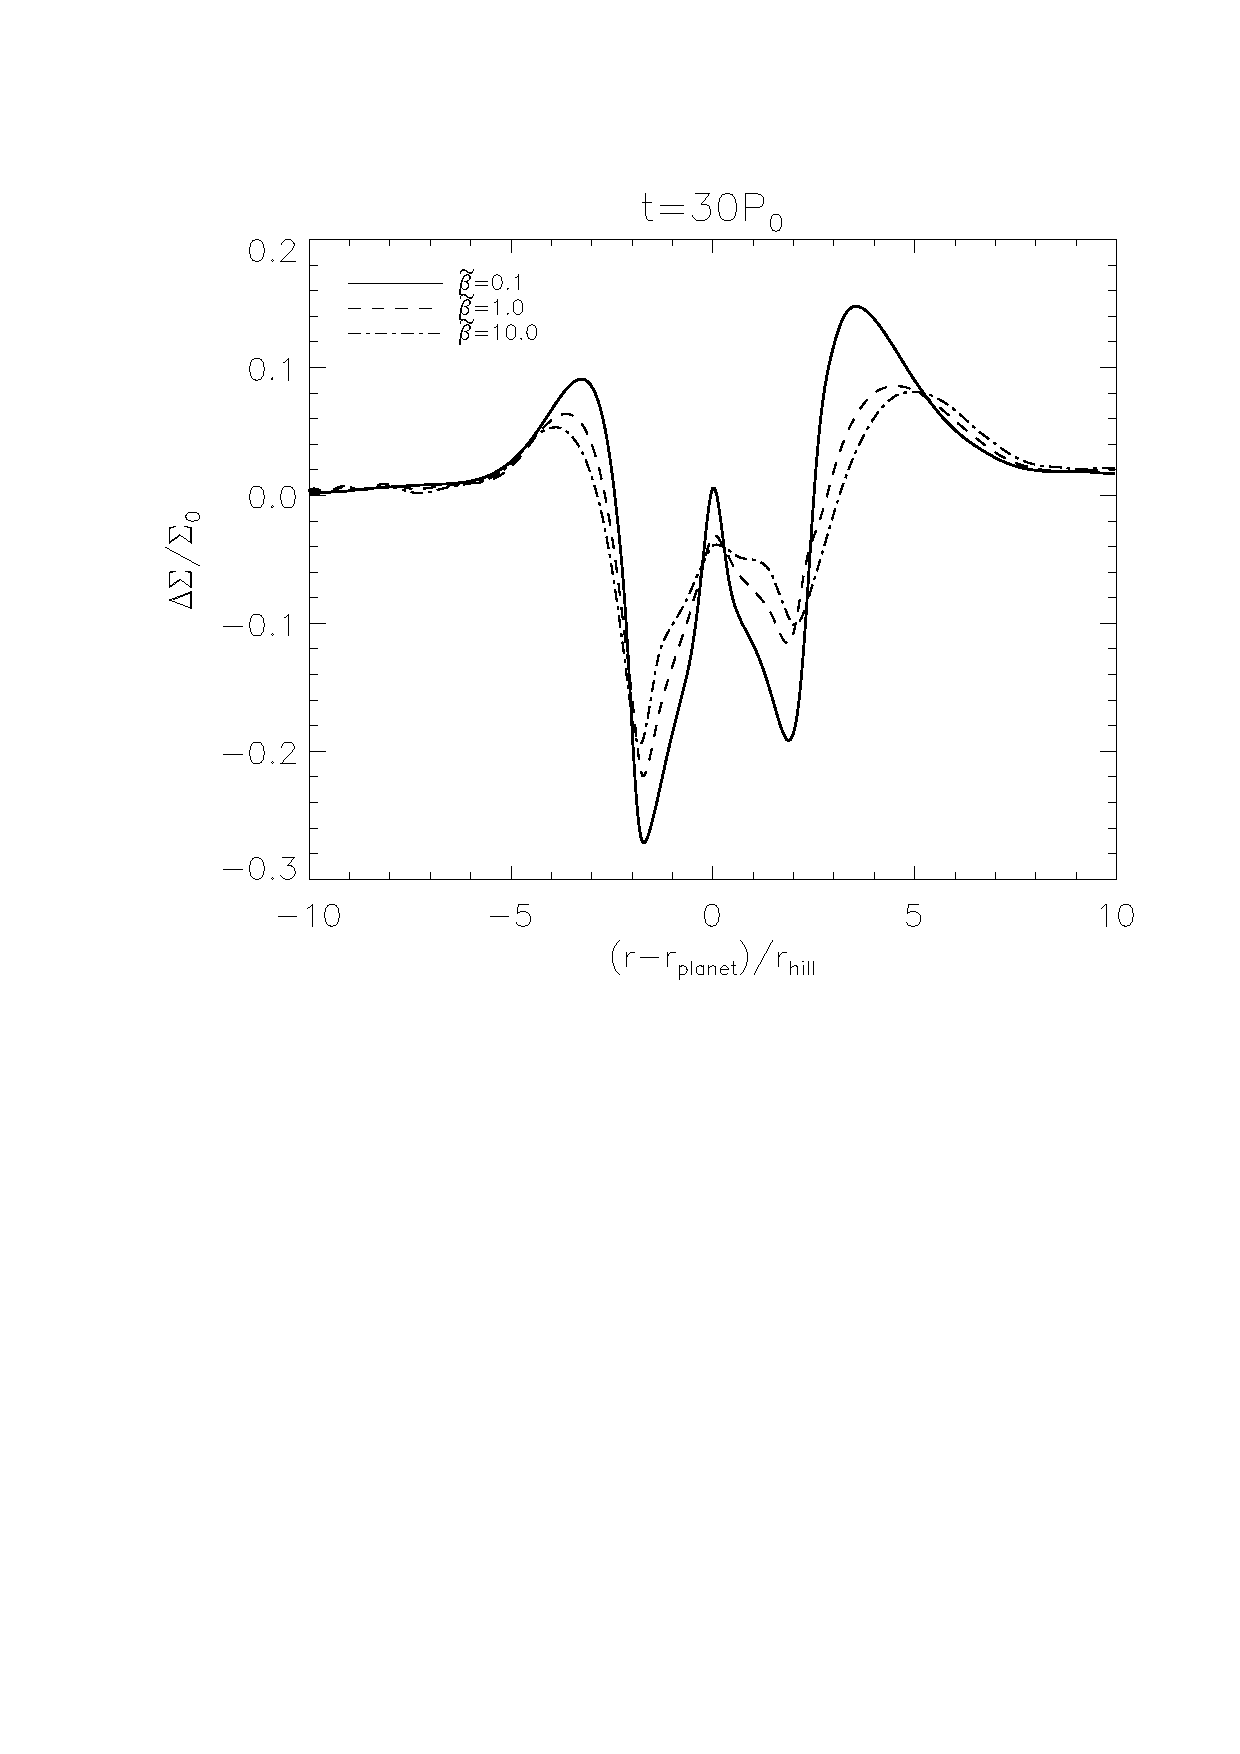
\includegraphics[width=\linewidth,clip=true,trim=0.5cm
    2cm 0cm 0cm]{figures/compare_sigma}
  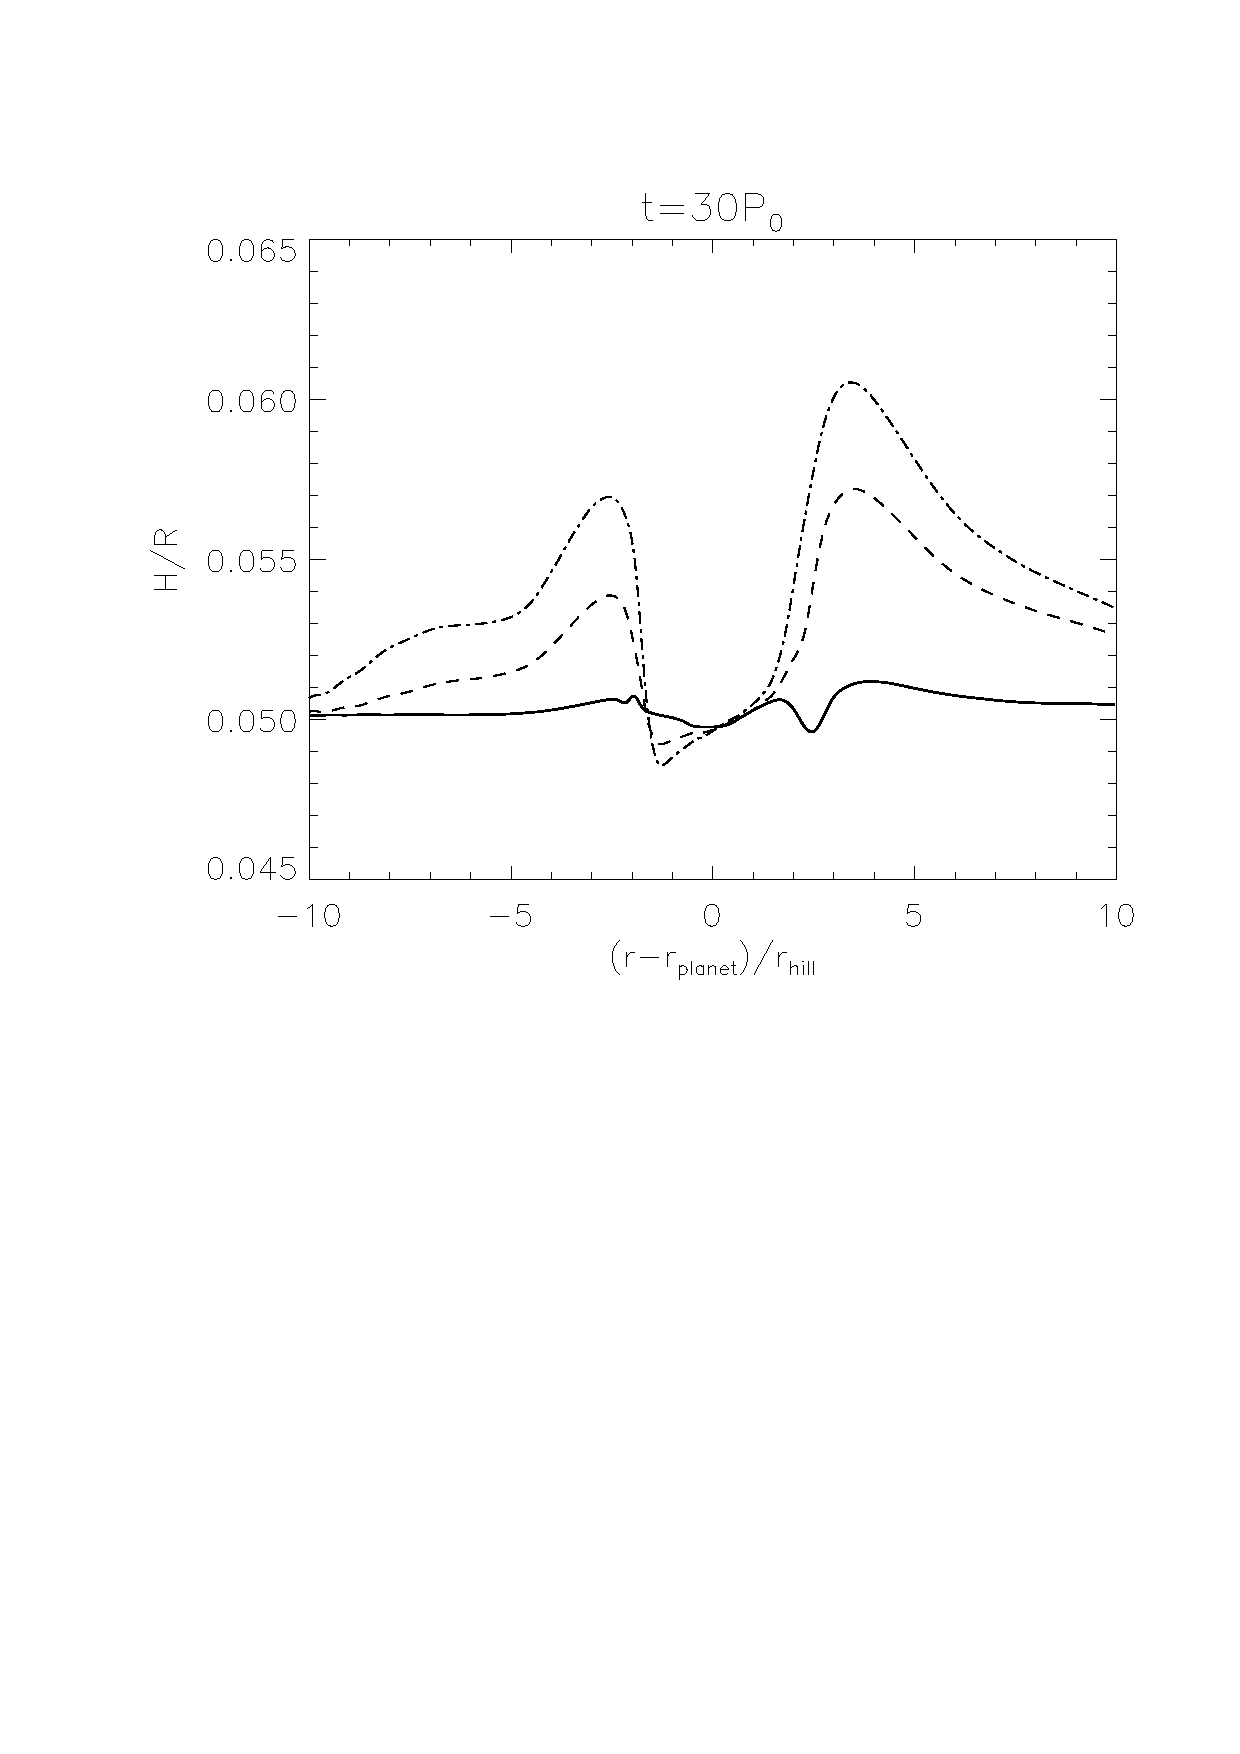
\includegraphics[width=\linewidth,clip=true,trim=0.5cm
    2cm 0cm 1cm]{figures/compare_aspectratio}
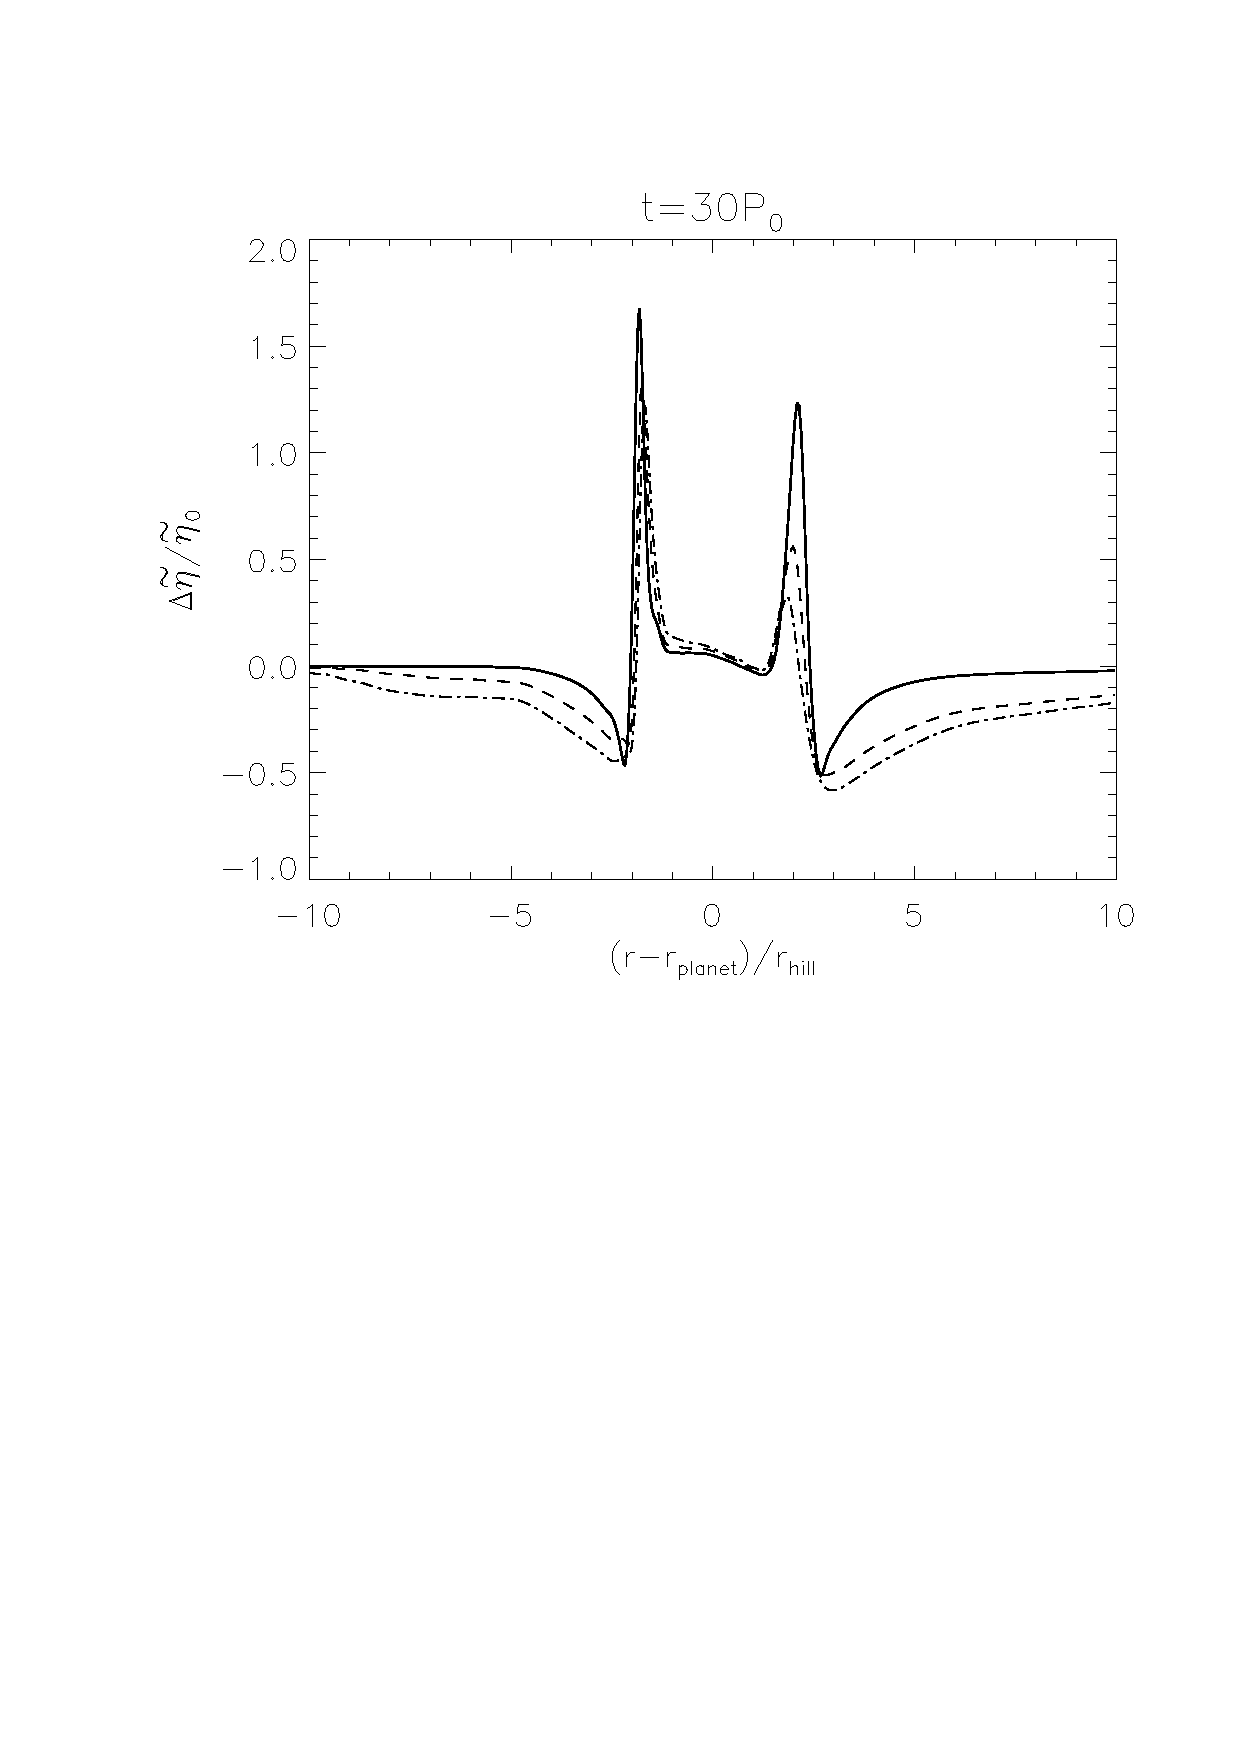
\includegraphics[width=\linewidth,clip=true,trim=0.5cm
    0.5cm 0cm 1cm]{figures/compare_gvortensity}
  \caption{Gap profiles at $t=30P_0$ for the intial partial gap opened
    before instability emerges for fast (solid), moderate
    (dashed), and slow cooling (dashed-dot). The relative surface density
    pertibation (top), disc aspectratio (middle) and generalized
    vortensity pertibation (bottom) are shown. \label{intial1D}}  
\end{figure}


%\begin{tabularx}{0.4\textwidth}{l*{10}{R}} \toprule
%  \multicolumn{11}{c}{$\tilde{\beta}=0.1$} \\ \midrule
%  m                    & 1 & 2 & 3 & 4 & 5 & 6 & 7 & 8 & 9 & 10  \\ 
 % $\gamma10^2/\Omega(r_o)$ & 6.56 & 6.82 & 6.73 & 5.78 & 6.00 & 6.38 & 5.97 & 5.62 & 4.61 & 3.36   \\ \bottomrule
%\end{tabularx}

%\begin{tabularx}{0.4\textwidth}{l*{5}{R}} \toprule
%  \multicolumn{6}{c}{$\tilde{\beta}=1.0$} \\ \midrule
%  m                    & 1 & 2 & 3 & 4 & 5  \\ 
%  $\gamma10^2/\Omega(r_o)$ & 1.27 & 1.28 & 1.35 & 1.01 & 0.61   \\ \bottomrule
%\end{tabularx}

\begin{table}
  \centering
  \caption{Dominant mode and growth rates for
    $\tilde{\beta}=0.1,1.0,10.0$ (fast, moderate, and slow cooling)
    values during `planet-off' simulations \label{modetable}} 
  \hfill
  \begin{minipage}{0.3\linewidth}
    \begin{tabularx}{\textwidth}{l R} 
      \multicolumn{2}{c}{$\tilde{\beta}=0.1$} \\ 
      \toprule
      $m$ & $10^2\gamma/\Omega(r_p)$ \\
      \midrule
      6 & 7.3 \\
      7 & 7.8 \\
      8 & 7.9 \\
      9 & 7.9 \\
      10 & 6.8 \\ 
      \bottomrule
    \end{tabularx}
  \end{minipage}
  \hfill
  \begin{minipage}{0.3\linewidth}
    \begin{tabularx}{\textwidth}{l R} 
      \multicolumn{2}{c}{$\tilde{\beta}=1.0$} \\ 
      \toprule
      $m$ & $10^2\gamma/\Omega(r_p)$ \\
      \midrule
      3 & 2.0 \\
      4 & 2.2 \\
      5 & 2.3 \\
      6 & 1.6 \\
      7 & 1.1 \\ 
      \bottomrule
    \end{tabularx}
  \end{minipage}
  \hfill
  \begin{minipage}{0.3\linewidth}
    \begin{tabularx}{\textwidth}{l R} 
      \multicolumn{2}{c}{$\tilde{\beta}=10.0$} \\ 
      \toprule
      $m$ & $10^2\gamma/\Omega(r_p)$ \\
      \midrule
      1 & 1.1 \\
      2 & 1.6 \\
      3 & 1.7 \\
      4 & 1.2 \\
      5 & 0.1 \\ 
      \bottomrule
    \end{tabularx}
  \end{minipage}
  \hfill
\end{table}

\subsection{Axisymmetric stability}
%Check that the gap profiles are stable against axisymmetric
%stability. Can use analytical criteria given in section 3.1 of Li et
%al (2000, ApJ, 533, 1023). No plot needed, just statements. 
%}
The intial planet-disc interaction form bumps and grooves in the gap profiles
which can potentially be unstable due to axisymmetric instabilities. The
generalised local axisymmetric stability condition is the Solberg-Hoiland
criterion,  
\begin{align}
  \kappa^2+N^2 \geq 0 
\end{align}
where
\begin{align}
 N^2=\frac{1}{\Sigma} \frac{\partial P}{\partial r}
 \left(\frac{1}{\Sigma} \frac{\partial \Sigma}{\partial
     r}-\frac{1}{\gamma P} \frac{\partial P}{\partial r}  \right) 
\end{align}
is the square of the Brunt-V\"ais\"al\"a frequency.  
%for the disk due to entropy
%variation which is non-zero for non-adiabatic models such as being
%considered. 
At the outer gap edge $r=r_p+2.5r_h$,  where the RWI is excited
(see below), we find $\kappa^2 + N^2$ reaches local minimum with a value
$\sim 0.002$ (code units) for all $\tilde\beta$. The
Brunt-V\"ais\"al\"a frequency is $N\sim 10^{-5}$. The Solberg-Hoiland
criteria is similary satisfied for the entire disc throughout the
simulations. % with little change of values. 
Thus for all values of $\tilde\beta$ the planet-induced gaps are
stable to axisymmertic instabilities. 

\subsection{Non-axisymmetric instability}\label{linear}
%{\bf present `planet-off' simulations. one `fourier mode v.s. time'
%  plot to show growth of linear instability. do an adiabatic case (or
%  extremely long cooling time) to see the effect of heated gap edge
%  (i.e. temp doesn't go back to t=0 value too quickly)
%  compare growth rate and dominant
%  m as function of beta (table). 2D figs to contrast (also used to
%  show it's the minimum in generalized pv that goes unstable.    
%  result: increasing cooling time makes the gap
%  more stable, and favors lower m. note: the `basic state' should be
%  the system at t=30 after azimuthal average. linear results should
%  have small perturbations. 
%}

%After the azimuthal averaging, the small pertibation excites rapidly
%growing instabilities by the RWI. 

We now examine the evolution of the gap for $t>30P_0$, with the
planet potential switched off, but with an added surface density
perturbation. For all three cooling times $\tilde{\beta}=0.1,\, 1.0,\,
10$, we observe exponential growth of non-axisymmetric
structures. % after the 
%planet potential is switched off and the system subject to random
%perturbations.  
An example is shown in Fig. \ref{linearmodes} for 
$\tilde{\beta}=10$. We charcterize these
modes with an azimuthal wavenumber $m$ and growth rate $\gamma(m)$ as defined by
Eq.~\ref{fouriertransform}---\ref{growth}. Mode amplitudes were
averaged over $r-r_p\in[2,5]r_h$. Table \ref{modetable}
lists the growth rates measured during 
linear growth for 5 values of $m$ centred around the maximum. 

\begin{figure}
  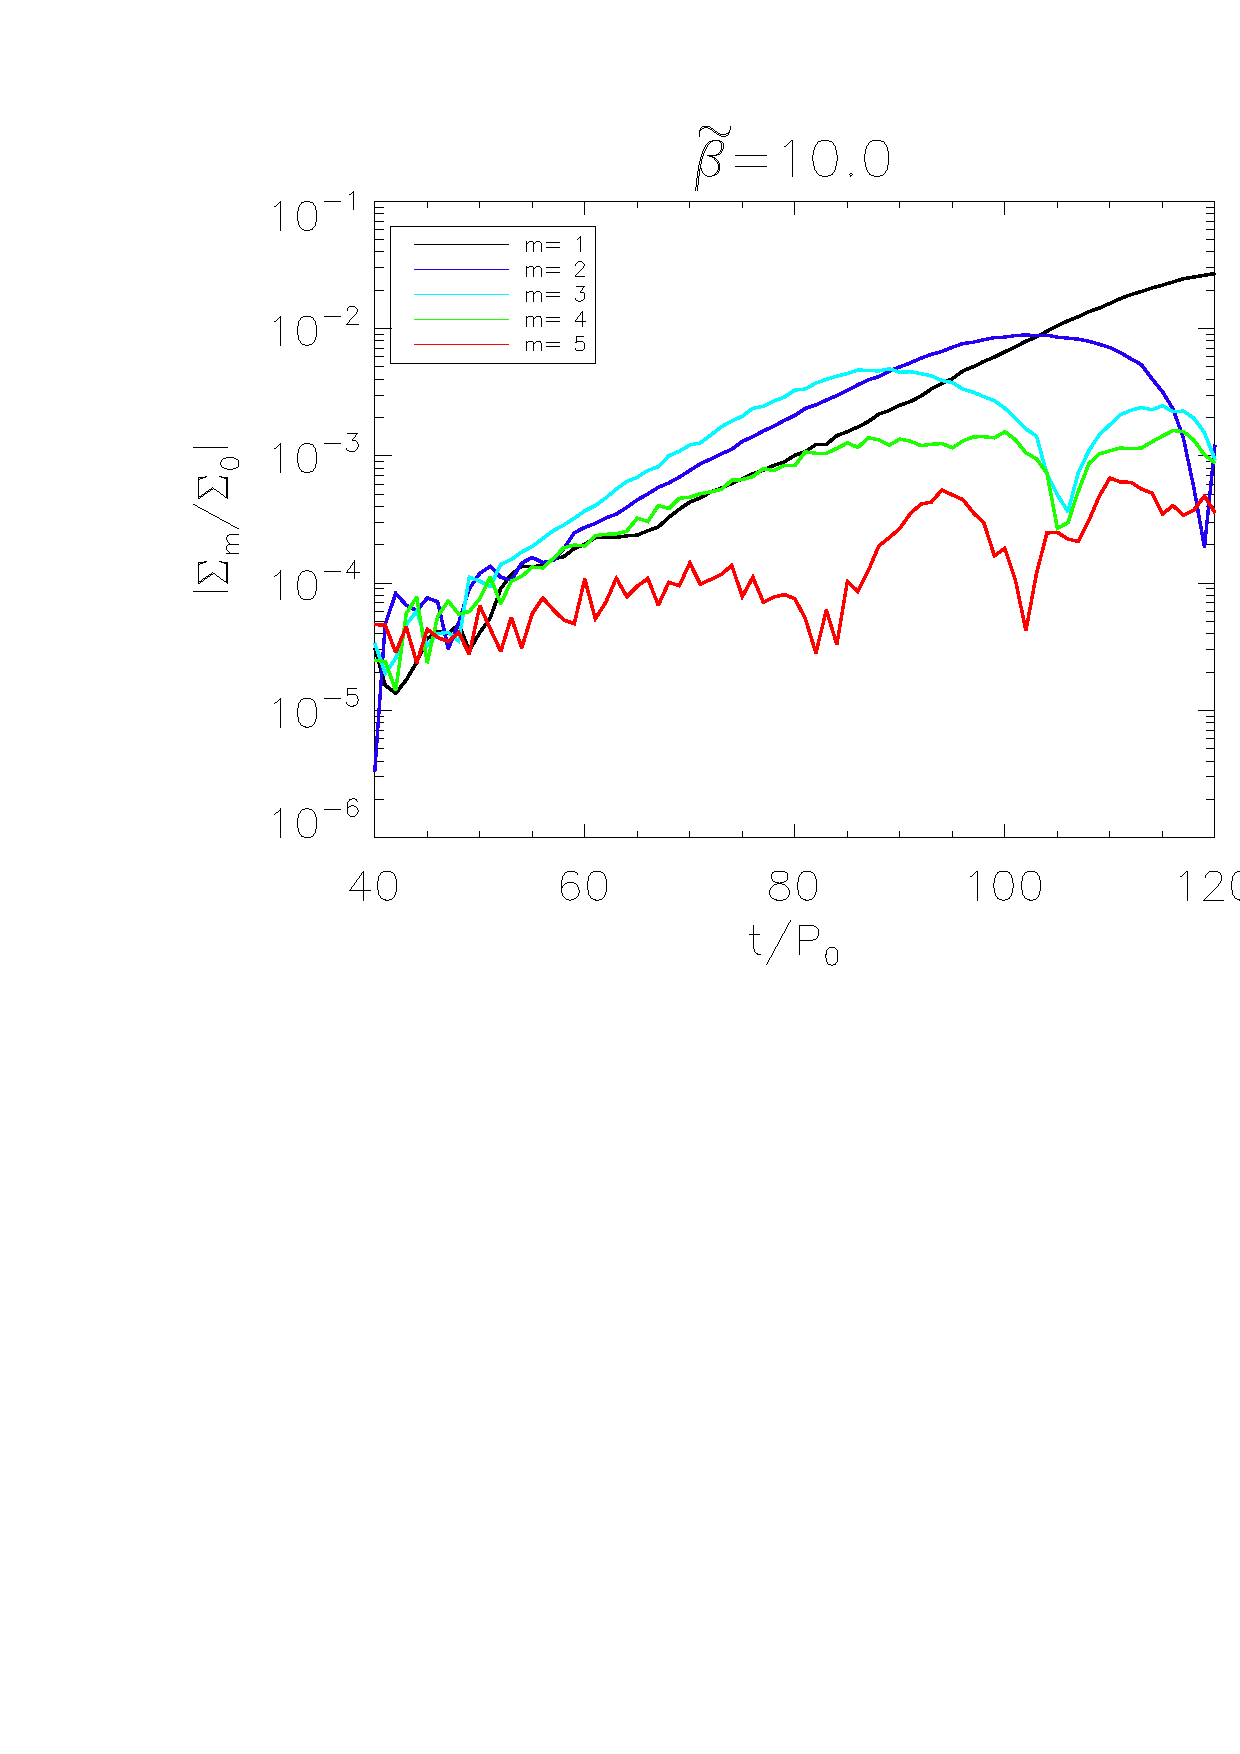
\includegraphics[width=\linewidth,clip=true,trim=1.2cm
  0cm 0cm 0cm]{figures/linear_stability}
  \caption{Evolution of azimuthal Fourier modes of disc surface
    density, non-dimenionlized by the initial axisymmetric background mode 
    $\Sigma_0(t=0)$ for the
    `planet-off' simulations with $\tilde{\beta}=10$. Colours correspond
    to different $m$ values. The $m=3$ component is the fastest growing
    mode during linear growth and has a corresponding
    $\gamma=0.017\Omega(r_p)$.\label{linearmodes}}
  % {\bf is the $\Sigma_0$ at t=0?} }  
\end{figure}

%%%%%%%%%%%%%%%%%%%%%%%%%%%%%%%%%%%%%%%%%%%%%%%%%%%%%%%%%%%%%%%%%%%%%%%

Table \ref{modetable} show that as
$\tilde{\beta}$ is increases from $ 0.1\rightarrow10$ the dominant
azimuthal Fourier mode decreases from $ m=9\rightarrow3$ and the
respective growth rate decreases from $ \gamma/\Omega(r_p)=0.079
\rightarrow 0.017$. However, despite two orders of magnitude increase in the
cooling time, the instability remains dynamical with characteristic  growth time
$\lesssim 10P_0$. Snapshots of the instability in for  
the different $\tilde\beta$ are shown in Fig \ref{2Dlinear}. 

These `planet-off' simulations show that gap edges become more stable with
longer cooling times. This is expected because larger $\tilde{\beta}$
result in hotter gap profiles at $t=30P_0$ with less pronounced
generalized vortensity minima. Stabilization with increased
cooling time is therefore due to a smoother basic state for the
instability, as it is more difficult for the planet to open a gap if
the disc is allowed to heat up. 
 
% which result in hotter gaps since the heating
%due
%This is as expected from the
%intial gap profiles, because 
% and the gap forming criteria discussed in the
%previous section. 

\begin{figure}
  \centering
  \subfigure{
    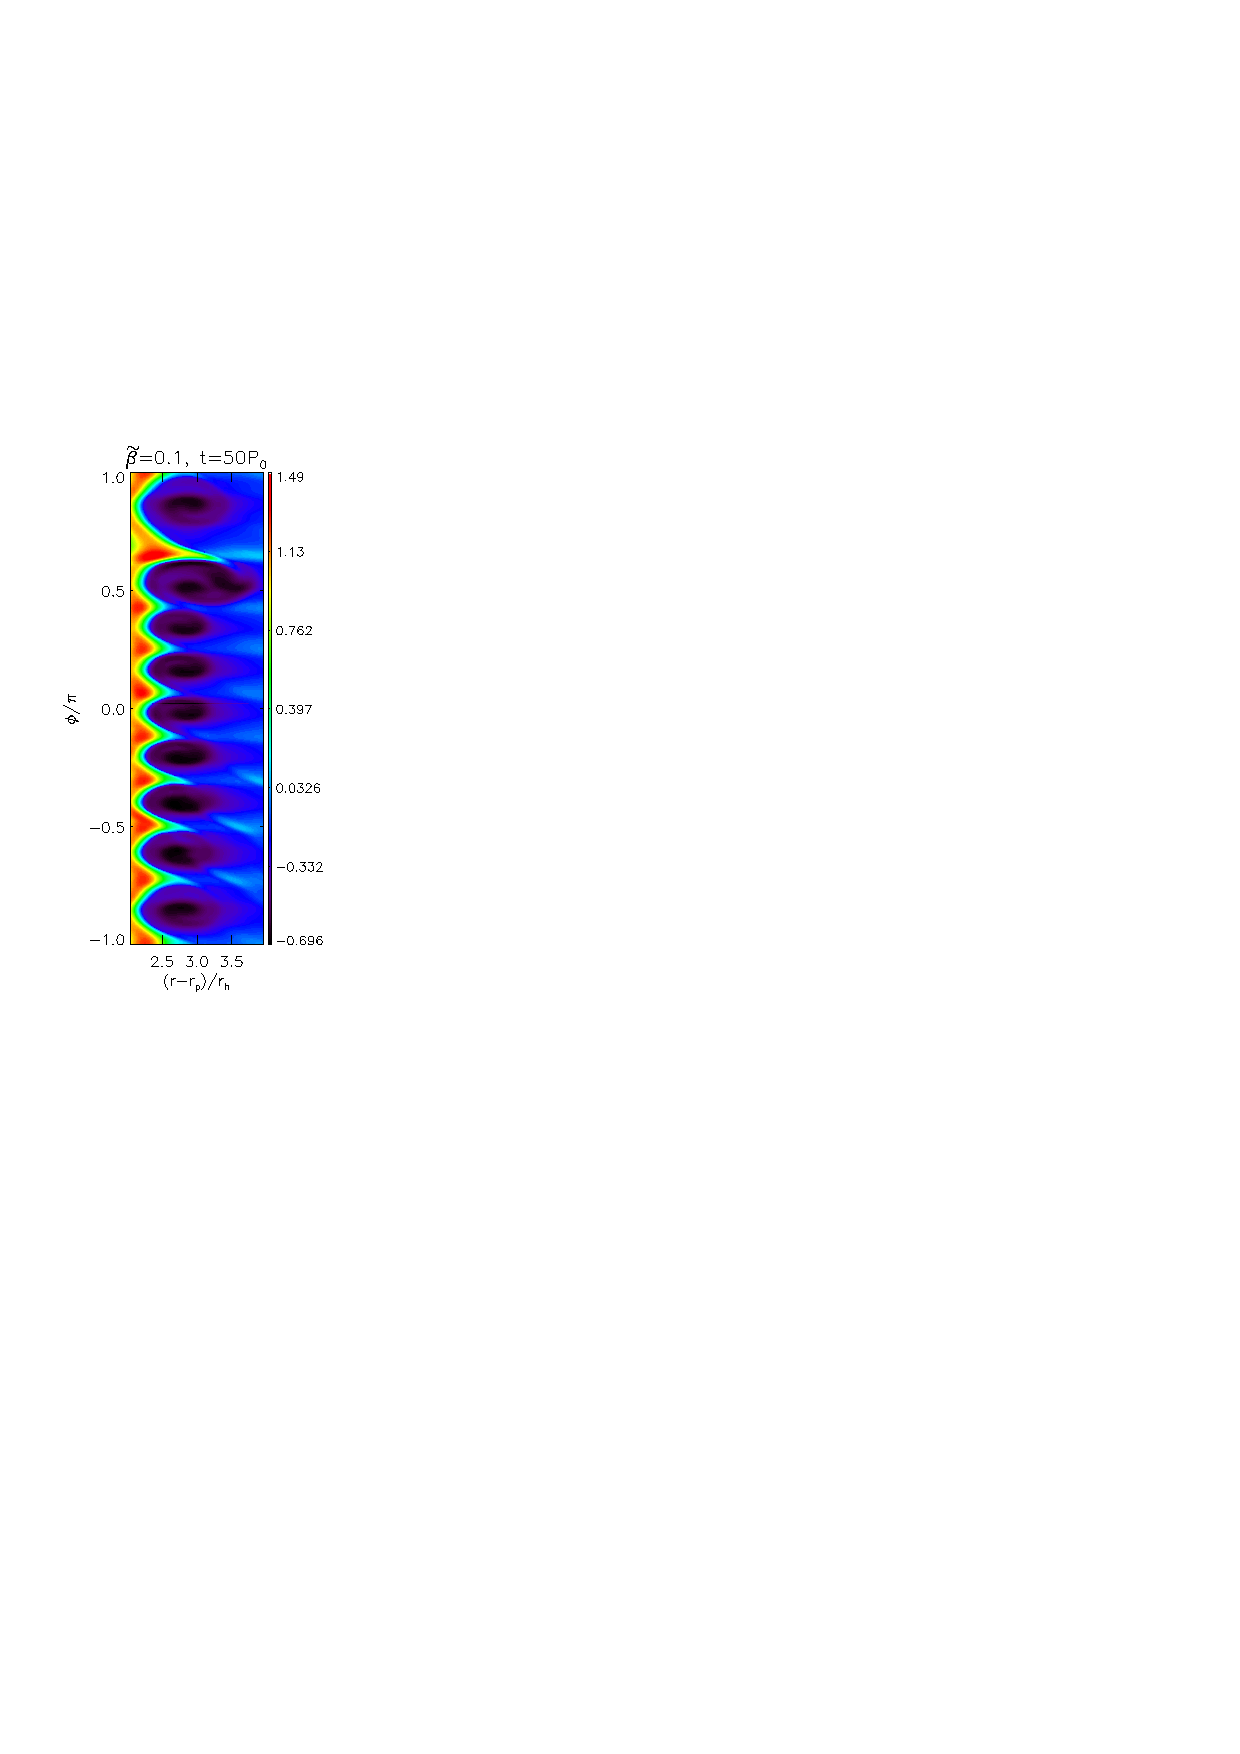
\includegraphics[width=0.3\linewidth]{figures/analysis_gvortensity50}
  }
\hfill
  \subfigure{
    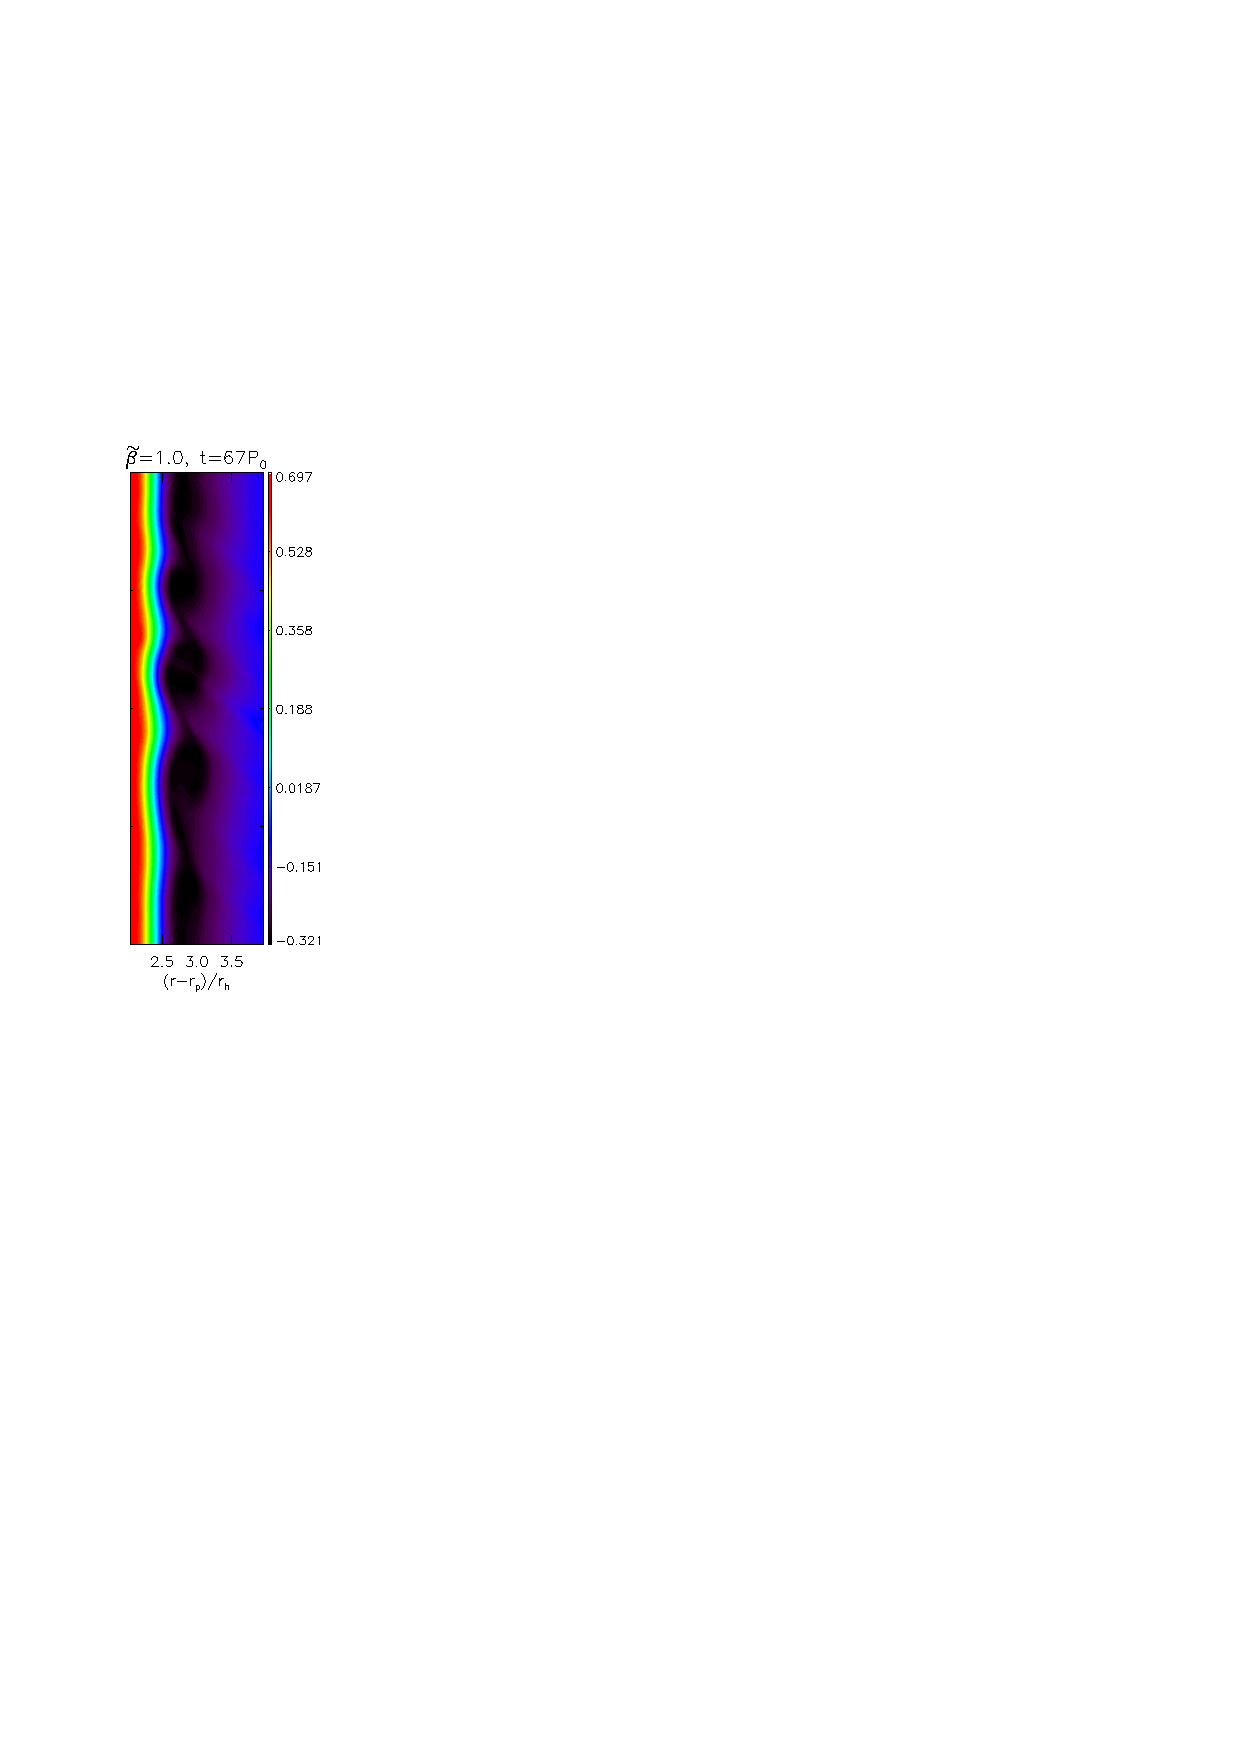
\includegraphics[width=0.3\linewidth]{figures/analysis_gvortensity67}
  }
\hfill
  \subfigure{
    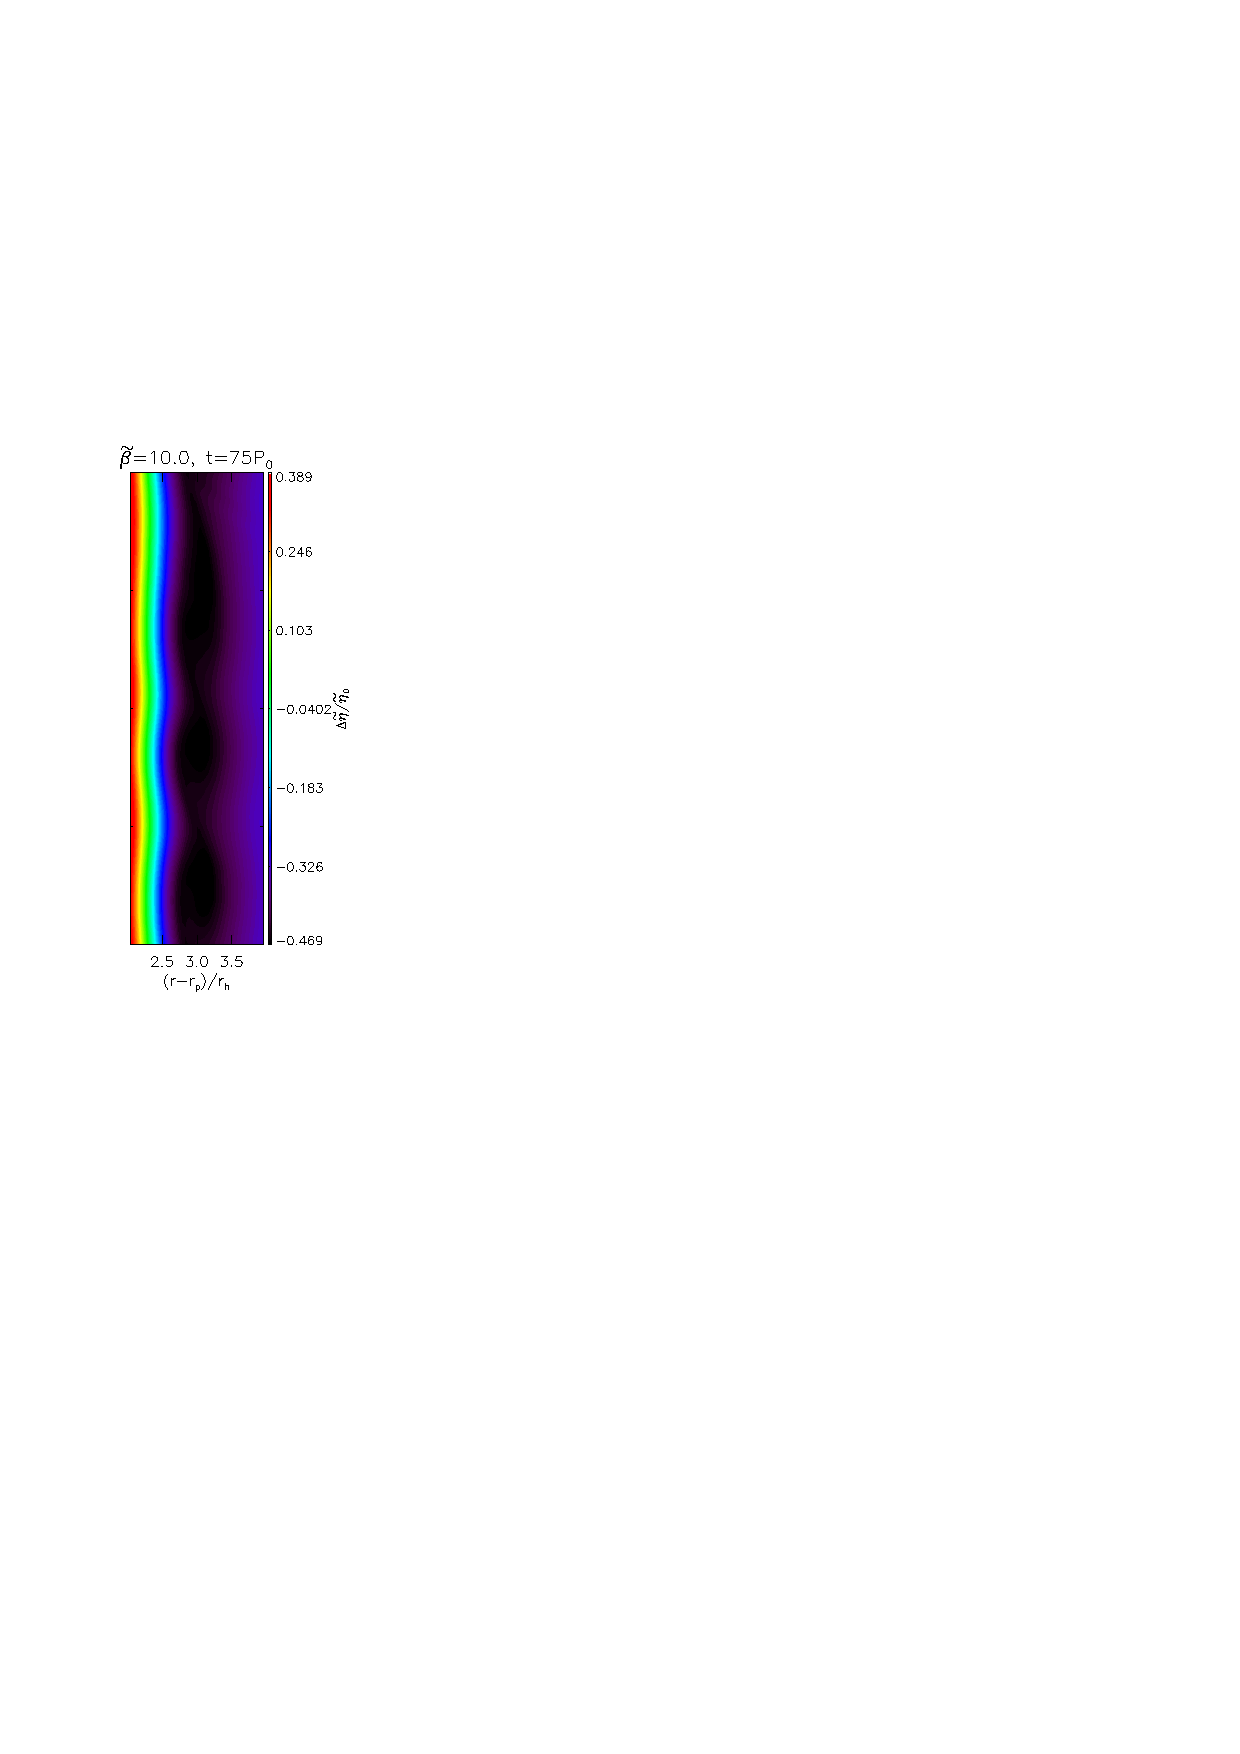
\includegraphics[width=0.3\linewidth]{figures/analysis_gvortensity75}
  }  
  \caption{Generalized vortensity perturbation (relative to $t=0$) for
    cases of $\tilde{\beta}=0.1,1,10$ (left,middle,right) during
    the growth of non-axisymmetric modes. The planet potential has
    been switched off.  The number of vortices
    decrease as $\tilde{\beta}$ increases. Note that snapshots are
    taken later for increasing $\tilde{\beta}$ because it takes longer
    for the vortices to grow and become visible with increasing cooling time. 
    % correspondingly increase to capture the longer growth phases of
    % the instabilities. 
    \label{2Dlinear} 
%{\bf I'm curious to know if plots clearer if
%      perturbations are measured relative to t=30? remember t=30 is
%      our reference state for instability. But we'll probably keep
%      these for consistency (later non-linear plots are all measure
%      with respect to t=0).}
  } 
\end{figure}

\subsubsection{Nearly adiabatic discs}
\label{adiabatic_section}
%{\bf a case with extrmely long cooling time (or adiabatic run) in
%  order to look at effect of heated gap edge.  prelim result: not
%  important, at t=30, gap edge only heats to $H/r\simeq0.06$ even for
%  purely adiabatic disk. change in $h$ not important for linear
%  perturbations (but important for setting up the basic state). 
%}
The above `planet-off' simulations are not formally linear
stability calculations, because the cooling time is shorter
than the instability growth time, 
%
%as we do not capture the effects of a heated
%disk on the instability growth. 
$t_c<\gamma^{-1}$.  
Thus the disk cools back to its intial temperature corresponding to
$h=0.05$ before or during the instability growth, so we do not
have a steady basic state to formulate a standard linear stability 
problem. %This means the disc temperture of $h=0.05$ in the the above cases 

In order to perform a proper linear stability analysis and capture the
effect of a heated gap edge during instability growth, we ran a simulation  with
$\tilde{\beta}=100$, corresponding to an almost adiabtaic disc.  
%To compare our 'planet-off' analysis with a true
%linear stability analysis 
In this simulation the cooling rate is slow enough that the gap 
temperature profile (e.g. middle panel of Fig. \ref{intial1D}) changes
only marginally over the instability growth timescale. %heat is
                                %retained/maintained.   

We find very similar gap profiles and mode growth rates for
$\tilde{\beta}=100$ as with $\tilde{\beta}=10$. The disc heats up to
values $h\simeq0.06$ in the nearly adiabatic case. This is close to
the original temperature of $h=0.05$, so linear growth rates are not expected
to change significantly %according to the linear theory presented in
\citep{li00}. 

According to \cite{li00}, increasing $h$ increases linear growth rates
of the RWI because it is pressure-driven. However, in the case 
of disc-planet interaction, increasing $h$ has a stabilizing effect
through the gap profile because it results in smoother gap
edges. The fact that we observe smaller growth rates as $h$ is
increased indicates that for planetary gaps, the importance of $h$ on
the \emph{linear} RWI is through setting up the gap profile, i.e. basic
state for the instability (as opposed to the linear response). 

%results in shallower gaps
%which is expected to be  

%the difference in growth rates between this and the
%original disc temperature of $h=0.05$ changes almost insignificantly
%as shown by linear theory \citep{li00}. 
%Although linear
%theory predicts higher growth rates with increasing $h$ 

%This indicate that a
%continuously hot gap edge is not as important for development of
%vortices as the heating effects on the formation of the intial gap
%state. 


%{\bf
%If there's time, do low resolution planet off simulations but keep the planet on
%until $t=40P_0$ or $50P_0$. Look at stability properties when the gaps
%are generally deeper (including the nearly adiabatic case). Although
%with the planet instability may already appear by $t=40P_0$, the
%azimtuhal average performed prior to perturbations will erase it.}

\subsection{Long term evolution} \label{nonlinearplanetoff} 
{\bf typical rossby numbers for these `planet-off' vortices? do
  stronger vortices (beta=0.1) dissipate faster? if we want to say the
  vortices dissipate viscously, then need to quote a viscosity
  (e.g. reynolds stress) and compute a viscous time and compare to the
  observed decay time. Or attribute to numerical viscosity. It might
  be simplest to just say the vortices decay without the planet. This
  section is mainly used to contrast with planet-on simulations, so
  don't need to go into detail. 
}

We also extended these `planet-off' simulations well into the non-linear
regime. After the linear growth phase of the vortices, vortex merging
takes hold on timescales of up to $150P_0$, until there is one vortex
left. We find the vortex merging
time is depedendent on the growth rates of the modes and saturation
timescales, with the slowest growing modes in $\tilde\beta=10$ taking
the longest to merge.  

Fig.\ref{planetofflifetimeplot} shows evolution of the $m=1$ surface
density amplitude, which represents the post-merger single vortex. For
completeness we also ran intermediate cases with $\tilde{\beta}=0.5$
and $5.0$. The vortices simply decay, on a timescale of $O(10^3)$
orbits. We will see in the next section that this behaviour is very
different to when the planet potential is kept on. Interestingly,
though, vortices arising from the stronger instabilities (shorter
cooling times or lower $\tilde{\beta}$) decays faster.  

%Similar
%quasi-steady vortices form as in the cases with continuous planet interaction
%but the long-term behaviour is significantly
%different without the planet as seen in 
%The quasi-steady vortices formed have significantly lower density pertibations
%and now slowly decrease in amplitute in time as apposed to previously
%where their growth was supported by planet interactions. 
%The vortices simply
%dissipate viscously with dissipation rate decreasing with larger $\tilde\beta$.

%Non-linear observations were also made for the `planet-off'
%simulations.
% as the vortices grow as linear
% instabilities discussed previously. 

%The vortices are never found to undergo the drastic sudden dissipation effects
%that characterize the planet induced growing cases do.

\begin{figure}
  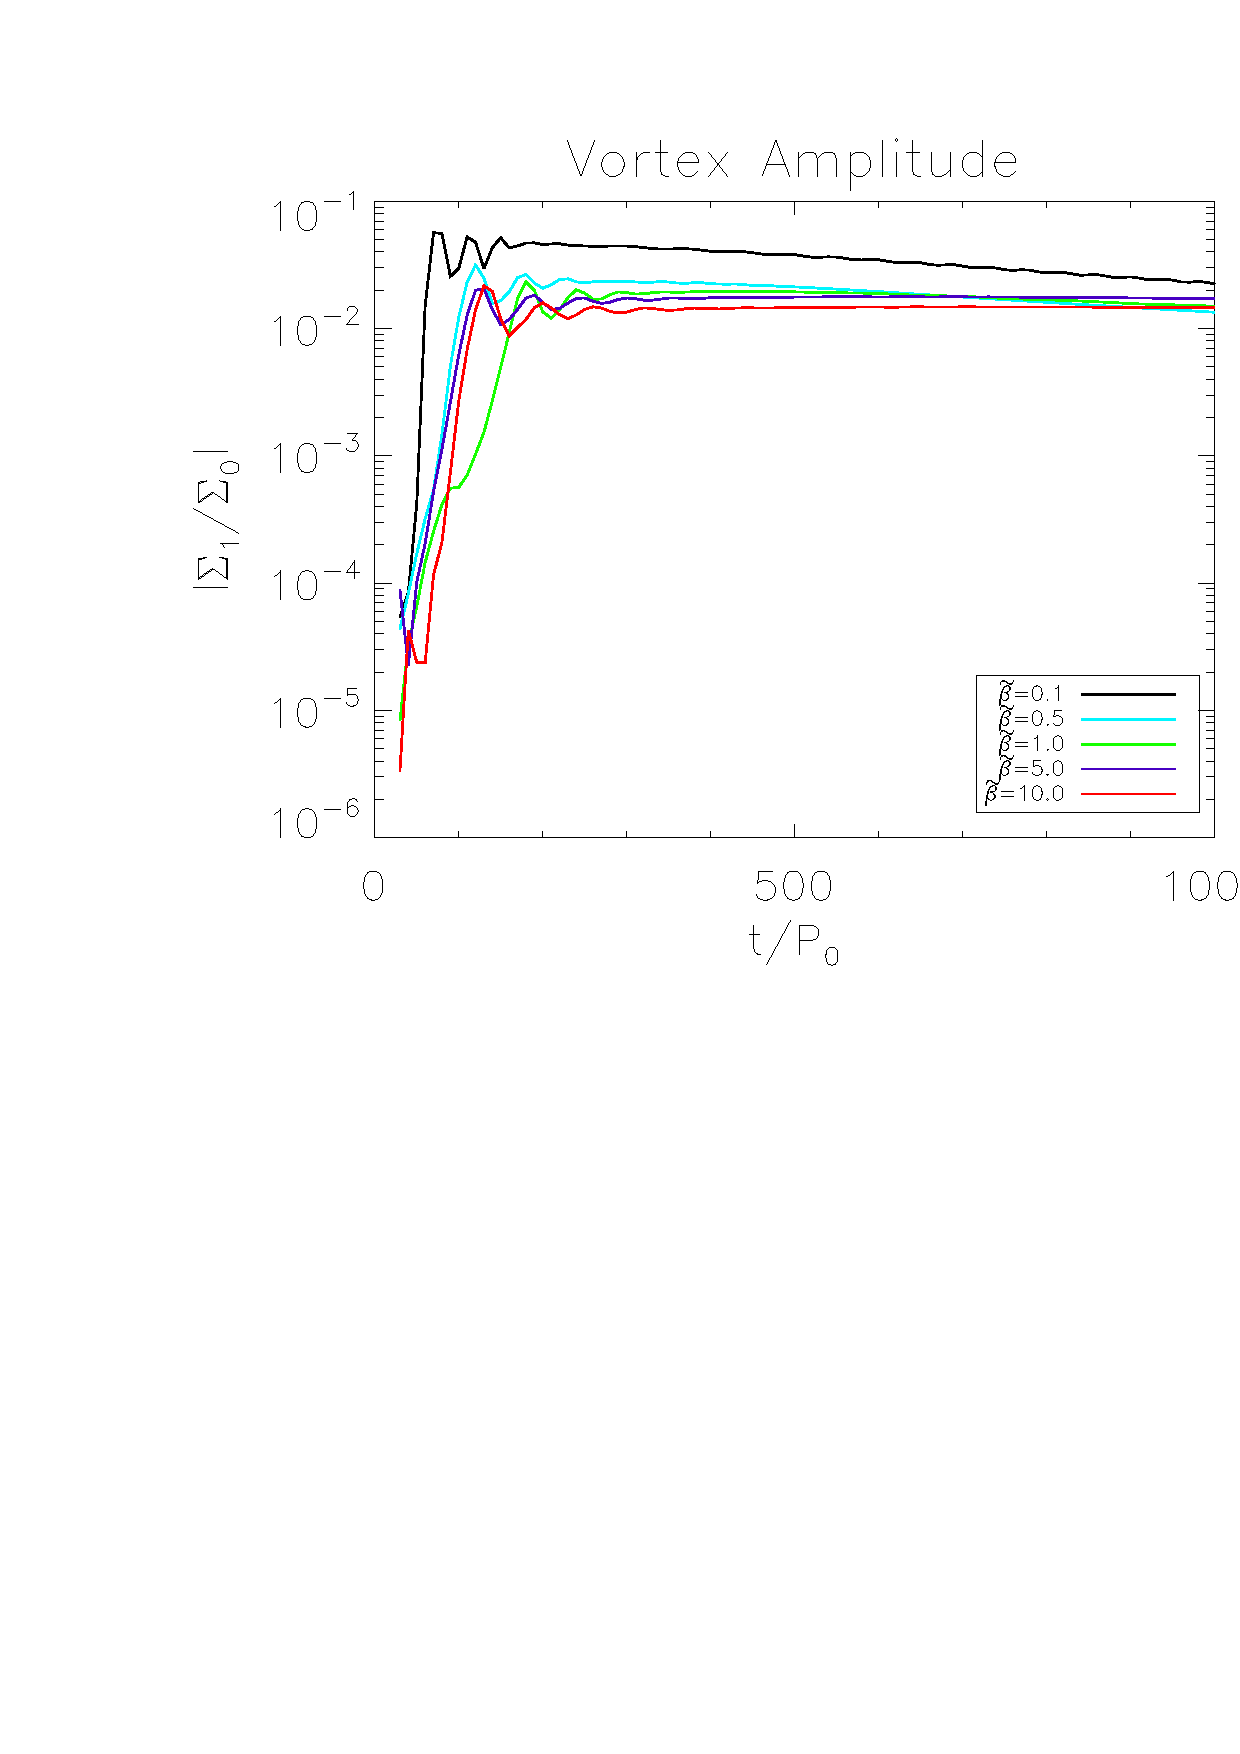
\includegraphics[width=\linewidth,clip=true,trim=0.5cm
  0cm 0cm 1.1cm]{figures/longterm_planetoff}
  \caption{Long term simulations without the planet potential after
    the gap is set up. The $m=1$ surface density component at the
    outer gap edge is shown.
  } \label{planetofflifetimeplot}
\end{figure}

%%%%%%%%%%%%%%%%%%%%%%%%%%%%%%%%%%%%%%%%%%%%%%%%%%%%%%%%%%%%%%%%%%%%%

\section{Non-linear evolution of
  gap-edge vortices with finite cooling time}\label{nonlinear} 
%{\bf main fig: vortex amplitude v.s. time for diff beta. enough data
%  to plot vortex lifetime v.s. beta? table: 
%  averaged quantities over quasi-steady state: aspect-ratio (to
%  compare with fu at al), rossby number (vortex strength
%  v.s. cooling?), maybe alpha visc. vortex size: visible difference?  
%  only inviscid cases. describe evolution of one case. main
%  conclusion: longer vortex lifetime with increasing cooling time (up
%  to some optimal timescale). vortex death: induced-shock and/or
%  smoothing the gap edge. describe simulation setup, resolution?
%  should mention that results consistent with lower-resolution prelim
%  runs. maybe torques? 
%}

We now examine long-term simulations of gap-edge vortices for
$\tilde{\beta}=0.1,0.5,1,5,10$. The planet potential is kept on
throughout.  
% up to a total of
%$2000P_0$. 
%Planets were left free to interact dynamiclly with the disk
%and vortices after $t=30P_0$ as apposed to previous section.  
We employ a grid with $(N_r,N_{\phi})=(512,1024)$ in order for these
simulations to be computationally feasible. We also use a larger
disc with $r_{\mathrm{out}}=45r_{\mathrm{in}}$ to minimize boundary
effects on vortex evolution, and apply open boundaries at
$r=r_\mathrm{in},\,r_\mathrm{out}$. We comment that lower-resolution
simulations with $(N_r,N_{\phi})=(256,512)$ were initially carried
out, which show similar behaviour and trends as the high-resolution
runs reported below.  

%where also done for the above $\tilde\beta$ values
%with the additional inclusions of $\tilde{\beta}=0.25,0.75,2.5,7.5$.
%Vortex evolution and behaviour are convergent with
%higher resolution simulations as discussed in this section.
% {\bf mention lower resolution preliminary runs - 
%similar results to those presented here (?). want to demonstrate convergence}

%An open boundry
%condition was used in the outer edge of
% allowing significant room for
%linblad resonances of the vortices. 

\subsection{Generic evolution} 
The linear growth of the RWI and vortex-formation is followed by 
vortex merging. We now find merging timescales independent of
$\tilde\beta$, and by $60P_o$ only one vortex remains.  
%as the growth of these modes are now 
%accelerated by planetary influence as apposed to `planet off' simulations.
% i.e. only the $m=1$ mode remains. 
The evolution of the amplitude of the $m=1$ surface density component,
averaged over $r-r_p\in[2,10]r_h$ is shown in Fig~\ref{lifetimeplot} 
for different $\tilde\beta$. 
{\bf any particular reason for the larger radial range for average?
  did we get bigger vortices?:Yes vortices get quite large in quais steady,
 changing the planet off averaging range to [2,10] changes the plots negligibly
 if we want to just use this value range for consistancy } 
% {\bf should state (also for planet-off runs)
% what the radial range is used for averaging the Fourier amplitudes} 

\begin{figure}
  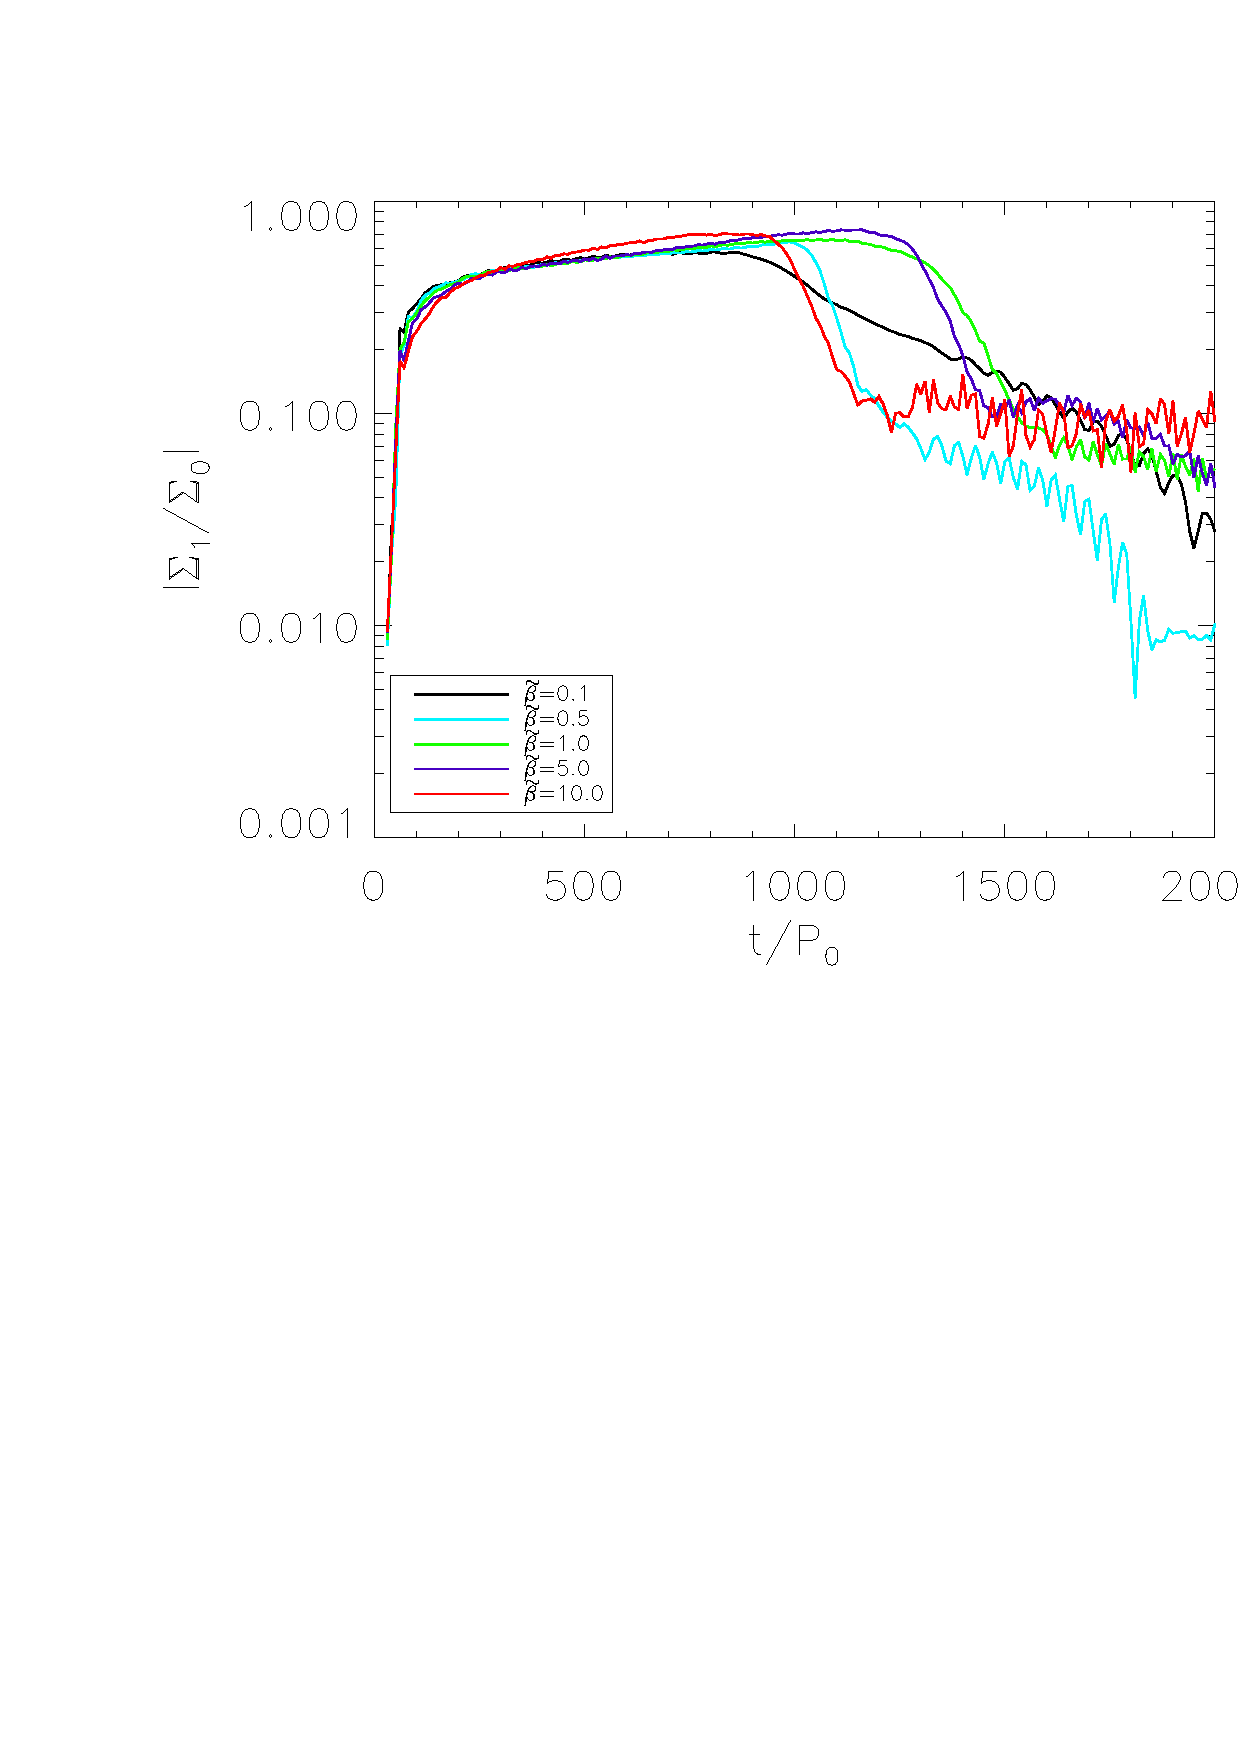
\includegraphics[width=\linewidth,clip=true,trim=0.5cm
  0cm 0cm 1cm]{figures/longterm_stability}
  \caption{Evolution of the $m=1$ surface density component,
    non-dimenionlised by the initial $m=0$ component, for long term
    simulations with the planet potential kept on. The case with 
    $\tilde\beta=5.0$ (red) gave the longest-living vortex. {\bf
      remember to update to 
      include vortex dissipation for all cases} \label{lifetimeplot}} 
\end{figure}

In all cases the system remains in a quasi-steady state for
$\gtrsim800P_0$ with a single vortex circulating 
the outer gap edge at the local Keplerian  
frequency. Fig. \ref{Vortex2D} shows a typical plot of the relative 
surface density perturbation in this state. During this stage, the 
vortex intensifies. As the vortex forms it has an initial 
Rossby number $Ro\approx-0.1$ for all $\tilde\beta$
(indicating anti-cyclonic
motion). As the $m=1$ amplitude grows the Rossby number also increases
in magnitude, 
%relative spin of the vortex
%continuously grows along with it
, reaching a characteristic value of $Ro\approx-0.4$ for all cooling
rates. {\bf is the the value reached just before decay for all cooling?:yes 
values peak in small range [-0.35,-0.45] for all beta}

The surface density perturbation (relative to $t=0$)  
can reach values of $\Delta\Sigma/\Sigma_0 \sim 7$ at the center of vortices
for all cases of $\tilde\beta$ in quasi-steady state, and
was found as high as $\Delta\Sigma/\Sigma_0 \sim 9$ for the 
$\tilde\beta=10$ case. This large increase in surface density is due 
vortex growth, since there is continuous generation of vorticity by
planet-disc interaction. This is supported by the observation that in
the previous simulations without the planet, the amplitude of
the post-merger vortex does not grow (Fig
\ref{planetofflifetimeplot}).  We remark that the increase in the
vortex surface density directly due to the pile-up of material at the
gap edge (because of gap-opening) is small: the average surface density
perturbation near the outer gap edge, $r\sim r_{p}+2.5r_h$, is 
$\langle\Delta\Sigma/\Sigma_0\rangle_\phi<1$.  

%{\bf is vortex merging affected by $\tilde{\beta}$? e.g. timescale
%  taken to reach one vortex as a function of cooling}
%{\bf for what cooling are these values quoted for? do
%  these values depend on cooling?}
% {\bf is the evidence for this the fact that growth is not observed in
%  planet-off simulations?}   
%{\bf note that there
%  are two origins for the surface density boost relative to $t=0$: 1) gap
%  formation, which increases the surface density at the location of
%  the instability (since they happen at surface density max., and 2)
%  vortex instability). what is the surface density boost relative to
%  the gap profile?}   


Interestingly, in most cases we observe a sudden drop in 
the $m=1$ amplitude within the simulation time, which occurs over
timescale between $20P_0$ to $70P_0$, i.e. much shorter than the duration of the
quasi-steady state. We did not find this dissipation timescale to
correlate with $\tilde\beta$. %but instead are paramtrized by vortex Mach numbers.
%{\bf is this dissipation timescale independent of cooling? Trend is
%based on mach values which dont follow linear trend }  
%Eventually
%the $m=1$ amplitudes are also characterized by 
%After these characteristic drops in vortex amplitude, the instability
%is never seen to reform at such large overdensities: the vortex surface
%densities are never larger than that due to the planetary wakes. 
We designate the time at which these amplitude drops as the lifetime 
of the quasi-steady vortex. After the vortices decay the RWI is 
not seen to be excited again and no vortices are seen to refrom within the
simulations time. 
{\bf Perhaps a snapshot of what the gap edge looks like after vortex death.
}
%The instability is not seen to emerge again after the intial vortex dissipation
% due to the smoothening out of the gap edge during dissipation by the
% transfer of density from the once tightly held vortex region to the surrounding disk and gap.  
% {\bf Discussed in next section:  question: does instability
%   actually happen again? if it does, but just weaker, that may be
%   because the first vortex has smoothed out the gap edge, so
%   instabilities following that would be weaker.}

\begin{figure}
  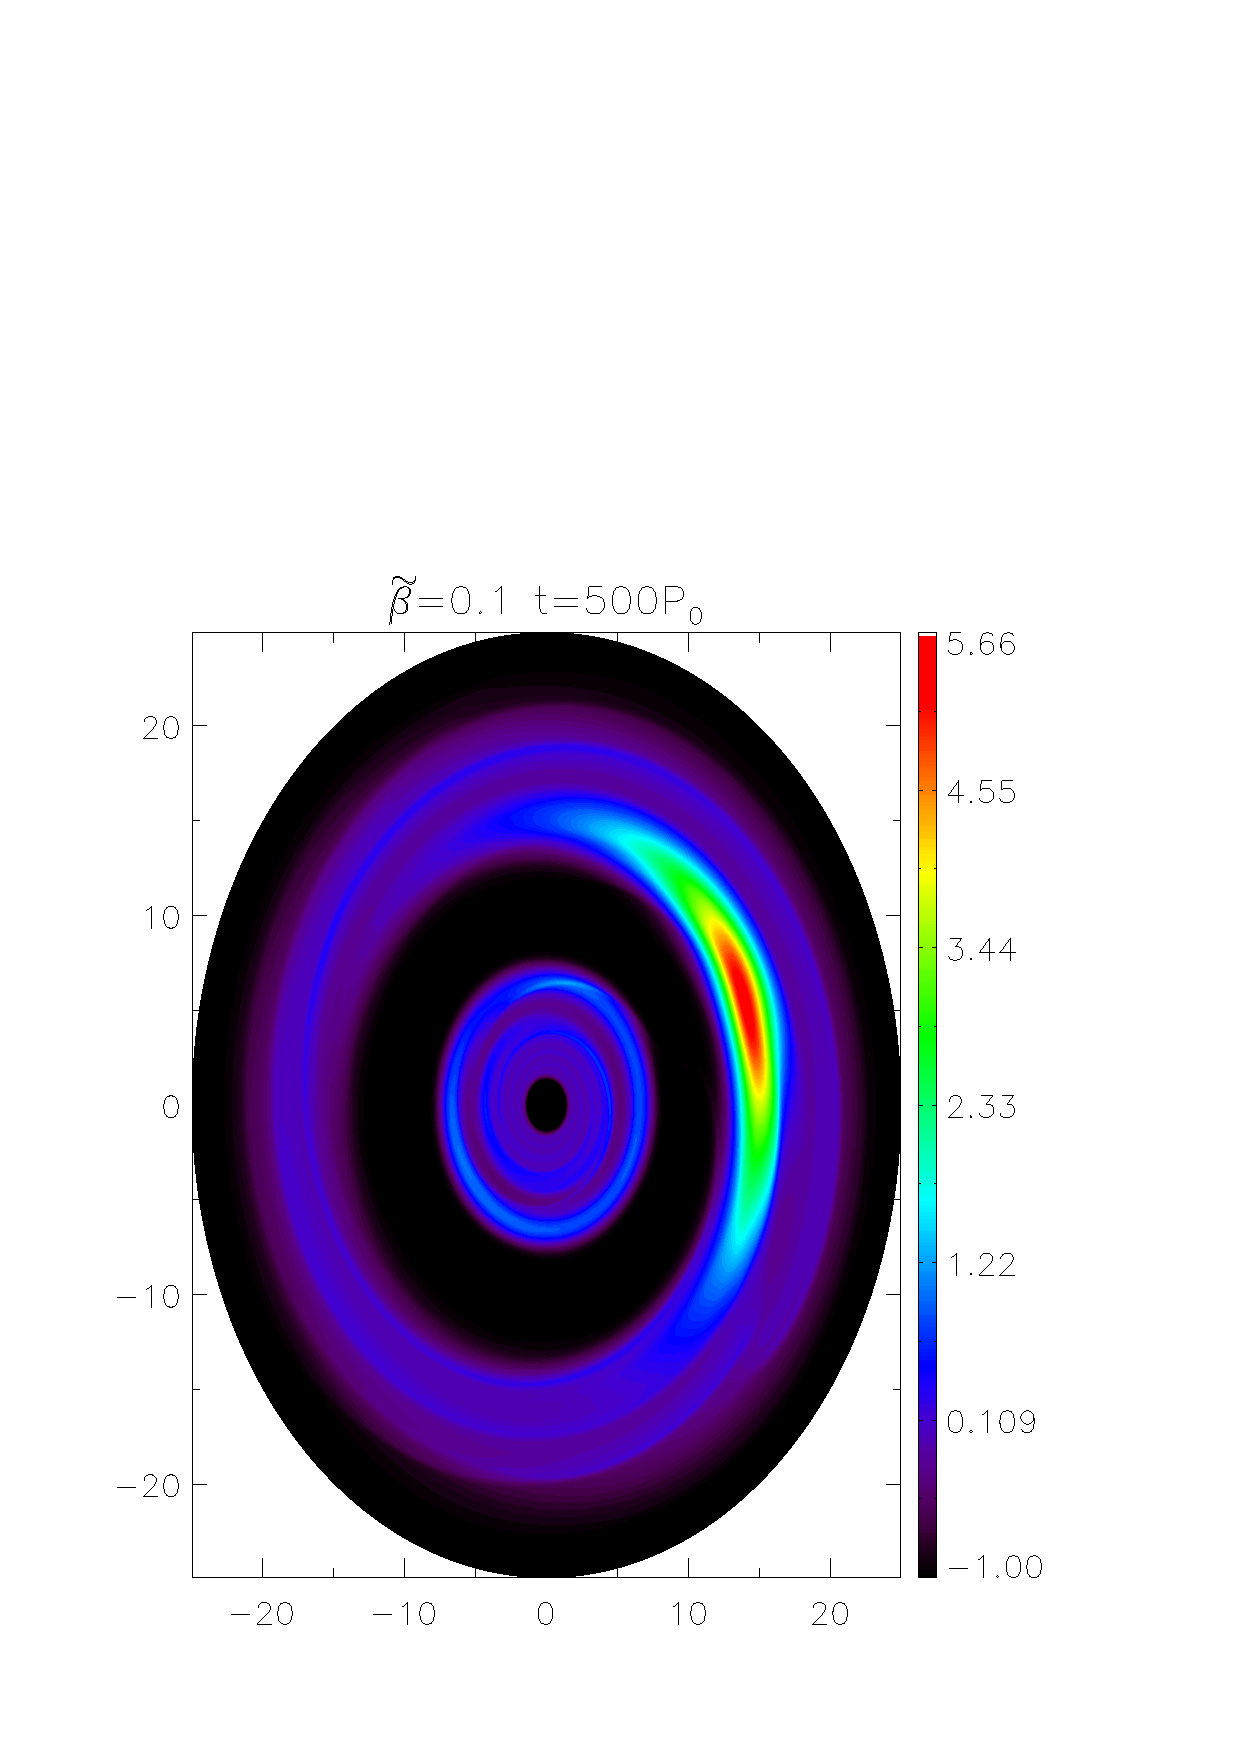
\includegraphics[width=\linewidth,height=\linewidth]{figures/vortex2D}
  \caption{Relative surface density perturbation for the
    $\tilde\beta=0.1$ case during quasi-steady state with a single
    vortex. The plots for other values of the cooling time
    $\tilde{\beta}$ are similar.
    % {\bf is this plot truncated? in the text it says the
    % domain goes to $r=45$?}
    % The large scale non-axisyemetric $m=1$ overdensity can be
    % seen. 
    \label{Vortex2D}} 
\end{figure}

\subsection{Additional analysis on vortex dissipation}
{\bf are these high resolution results? vortex lifetime in snapshots
  not consistent with amplitude plots}
%Conjecture: vortex death due to vortex shocking the system and
%dissipating its energy. discuss one case. here we want to explain or
%suggest why vortices die} 
%Rossby values have dynamics that are coupled with the lifetime and
%$m=1$ amplitude of the vortices.
In this subsection we examine the sudden vortex decay observed in our
simulations in more detail. Fig. \ref{shockplot} show snapshots
of the vortex leading up to its decay for the case $\tilde{\beta}=1$. 
The surface density perturbation and the surface density gradient are
shown. In quasi-steady ($t=700P_0$) the vortex is elongated, but becomes
more compact as it grows before decaying. {\bf rough estimate of
  vortex aspect-ratio in the three snapshots? 
  (length/width, by inspection is ok)}  

Notice in Fig. \ref{shockplot} the appearence of wakes extending from
either side of the vortex at $t=1300P_0$ as it grows. These 
wakes correlate with large gradients in surface density (bottom
panel), and are first seen in the later half of the quasi-steady state.       
% As the vortices grow in intensity wakes are seen to extend from them. 
During this phase the average value of the surface density gradient
along the wakes is $|\nabla\Sigma/\Sigma| \sim 4 $.{\bf quote something
  dimensionless, or say `in code units'}  
Just before the vortices start to decay, we observe this quantity
sharply increases to $ \sim 6 $, and remains around this value
until the vortex dies out, at which point the 
associated Rossby number quickly approaches zero.  

\begin{figure}
\subfigure{
    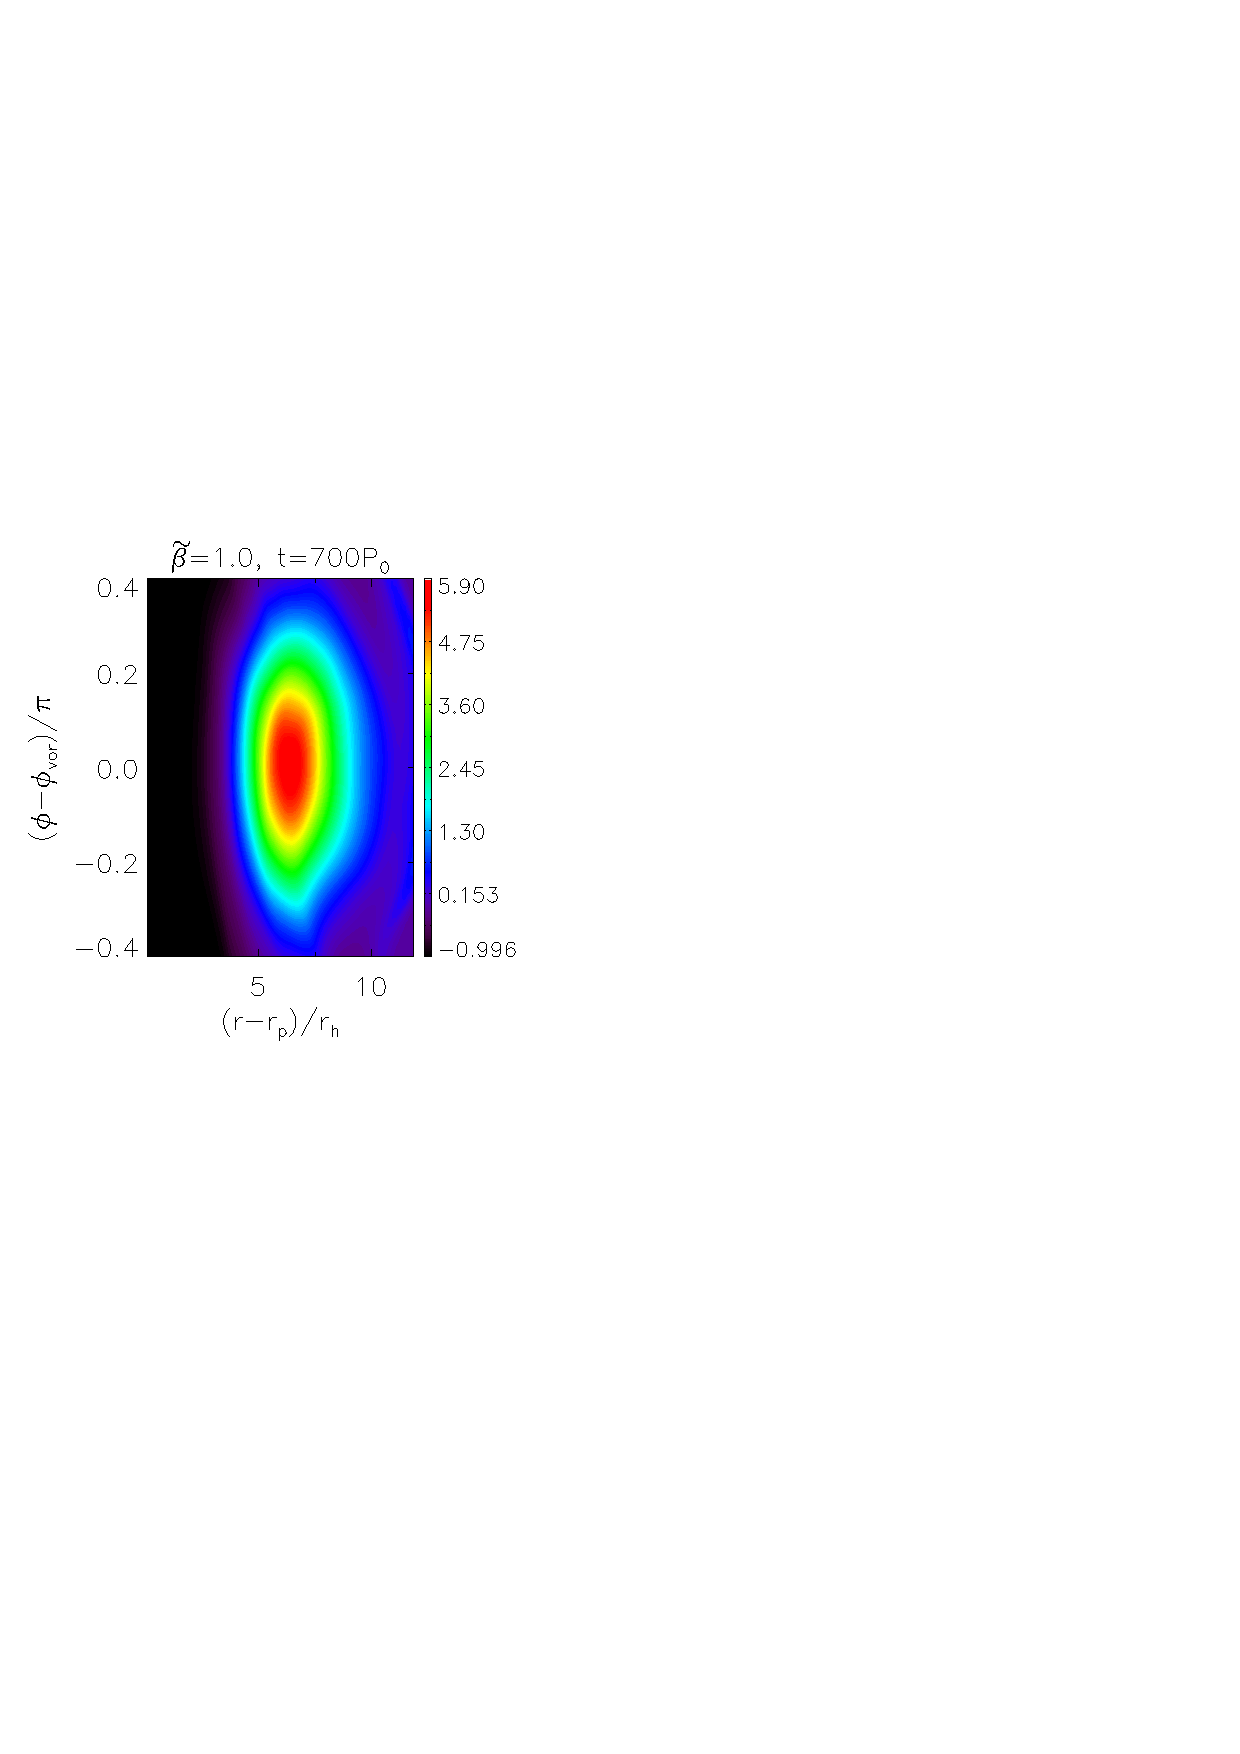
\includegraphics[width=0.3\linewidth]{figures/shock1}
  }
\hfill
  \subfigure{
    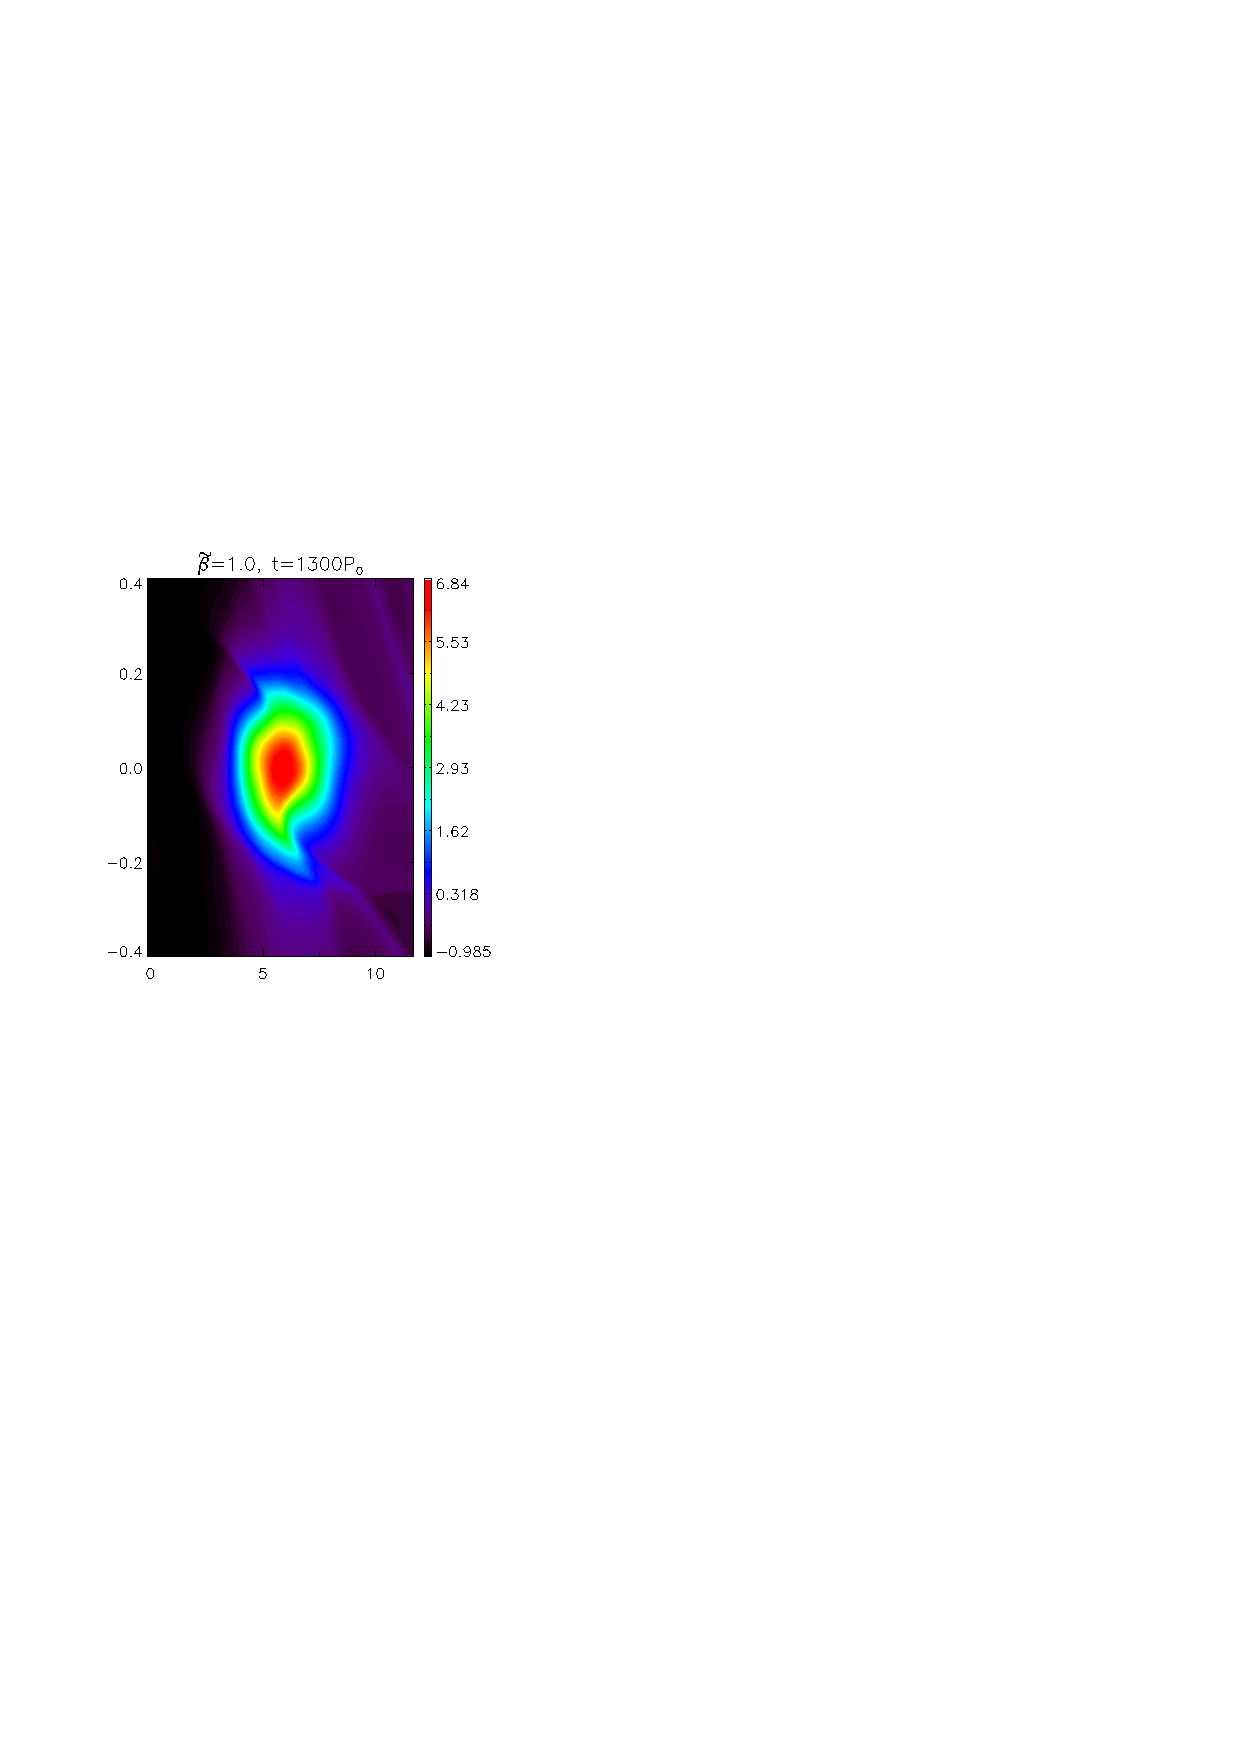
\includegraphics[width=0.3\linewidth]{figures/shock2}
  }
\hfill
  \subfigure{
    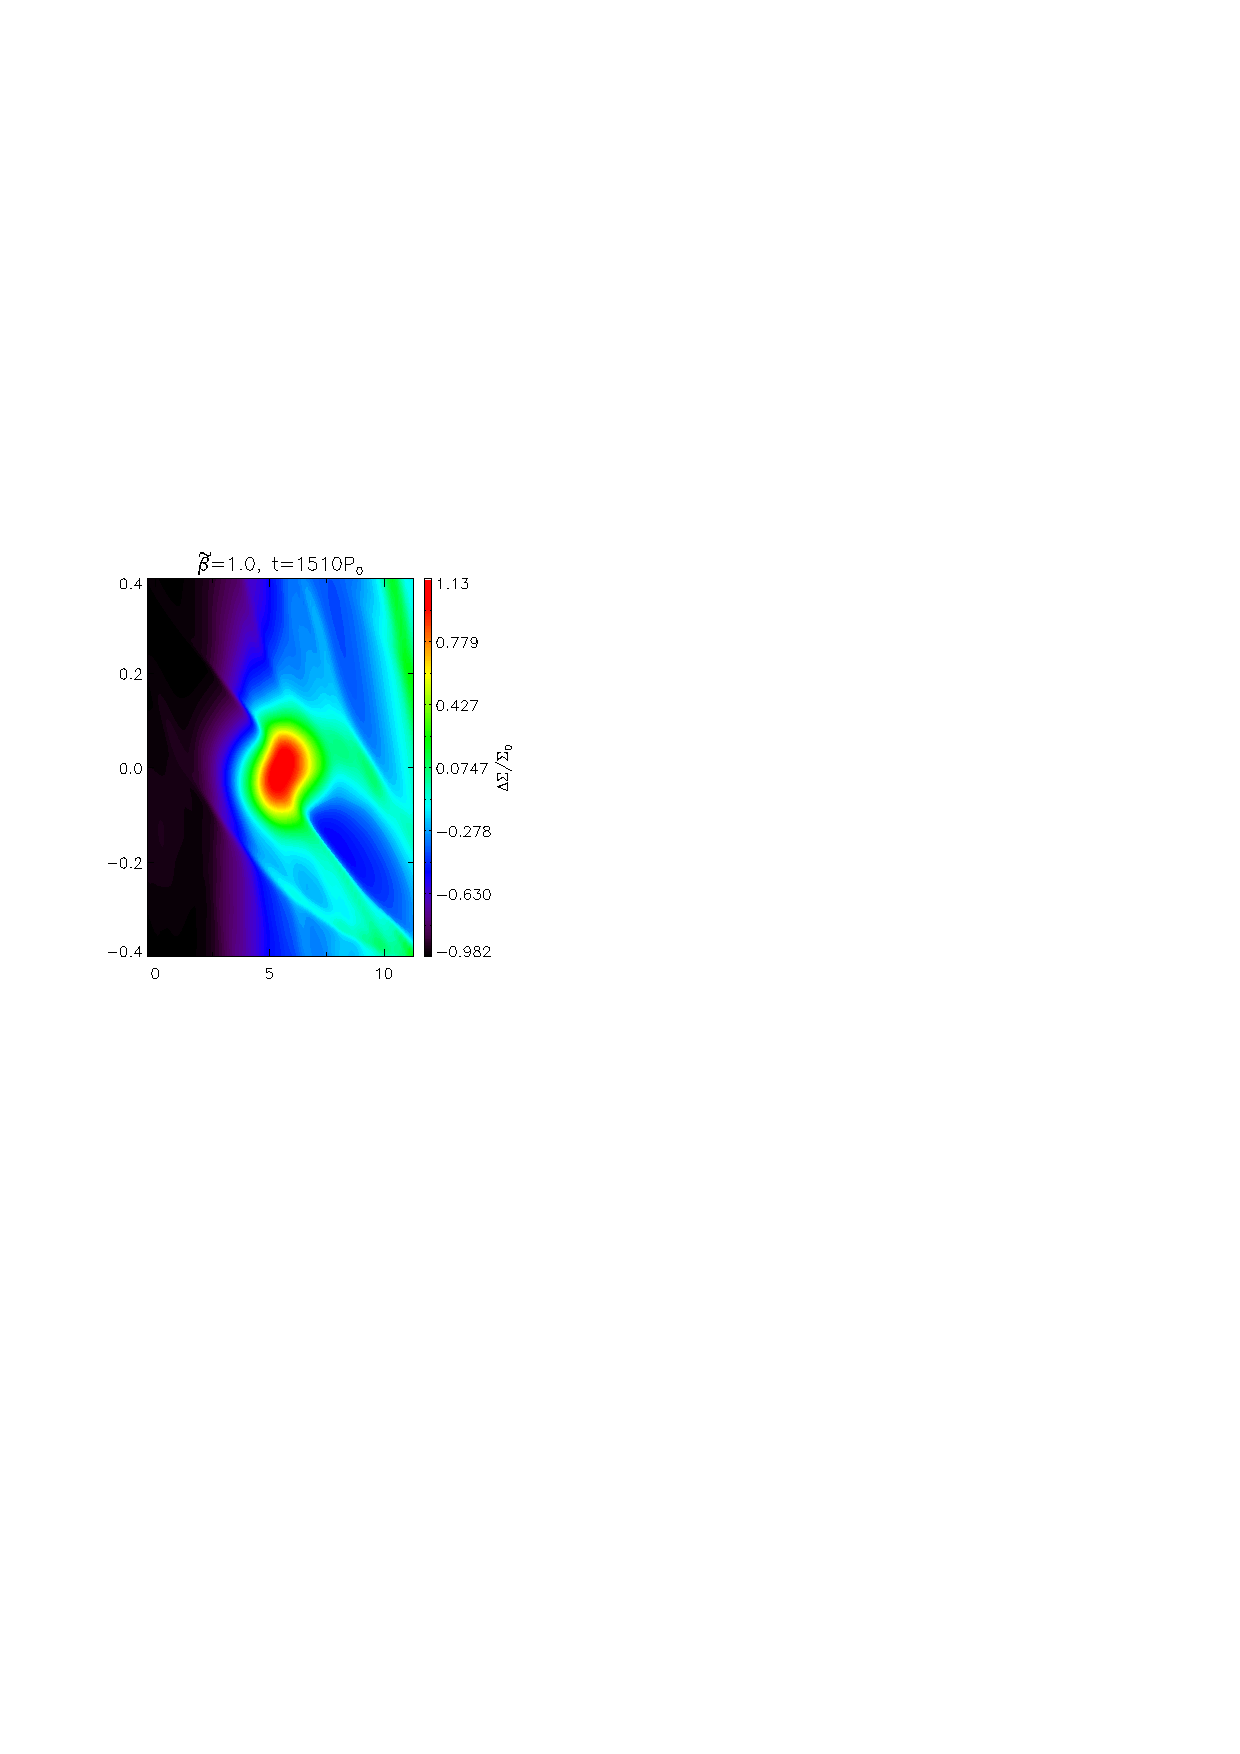
\includegraphics[width=0.3\linewidth]{figures/shock3}
  } \\[-0.98cm]
\subfigure{
    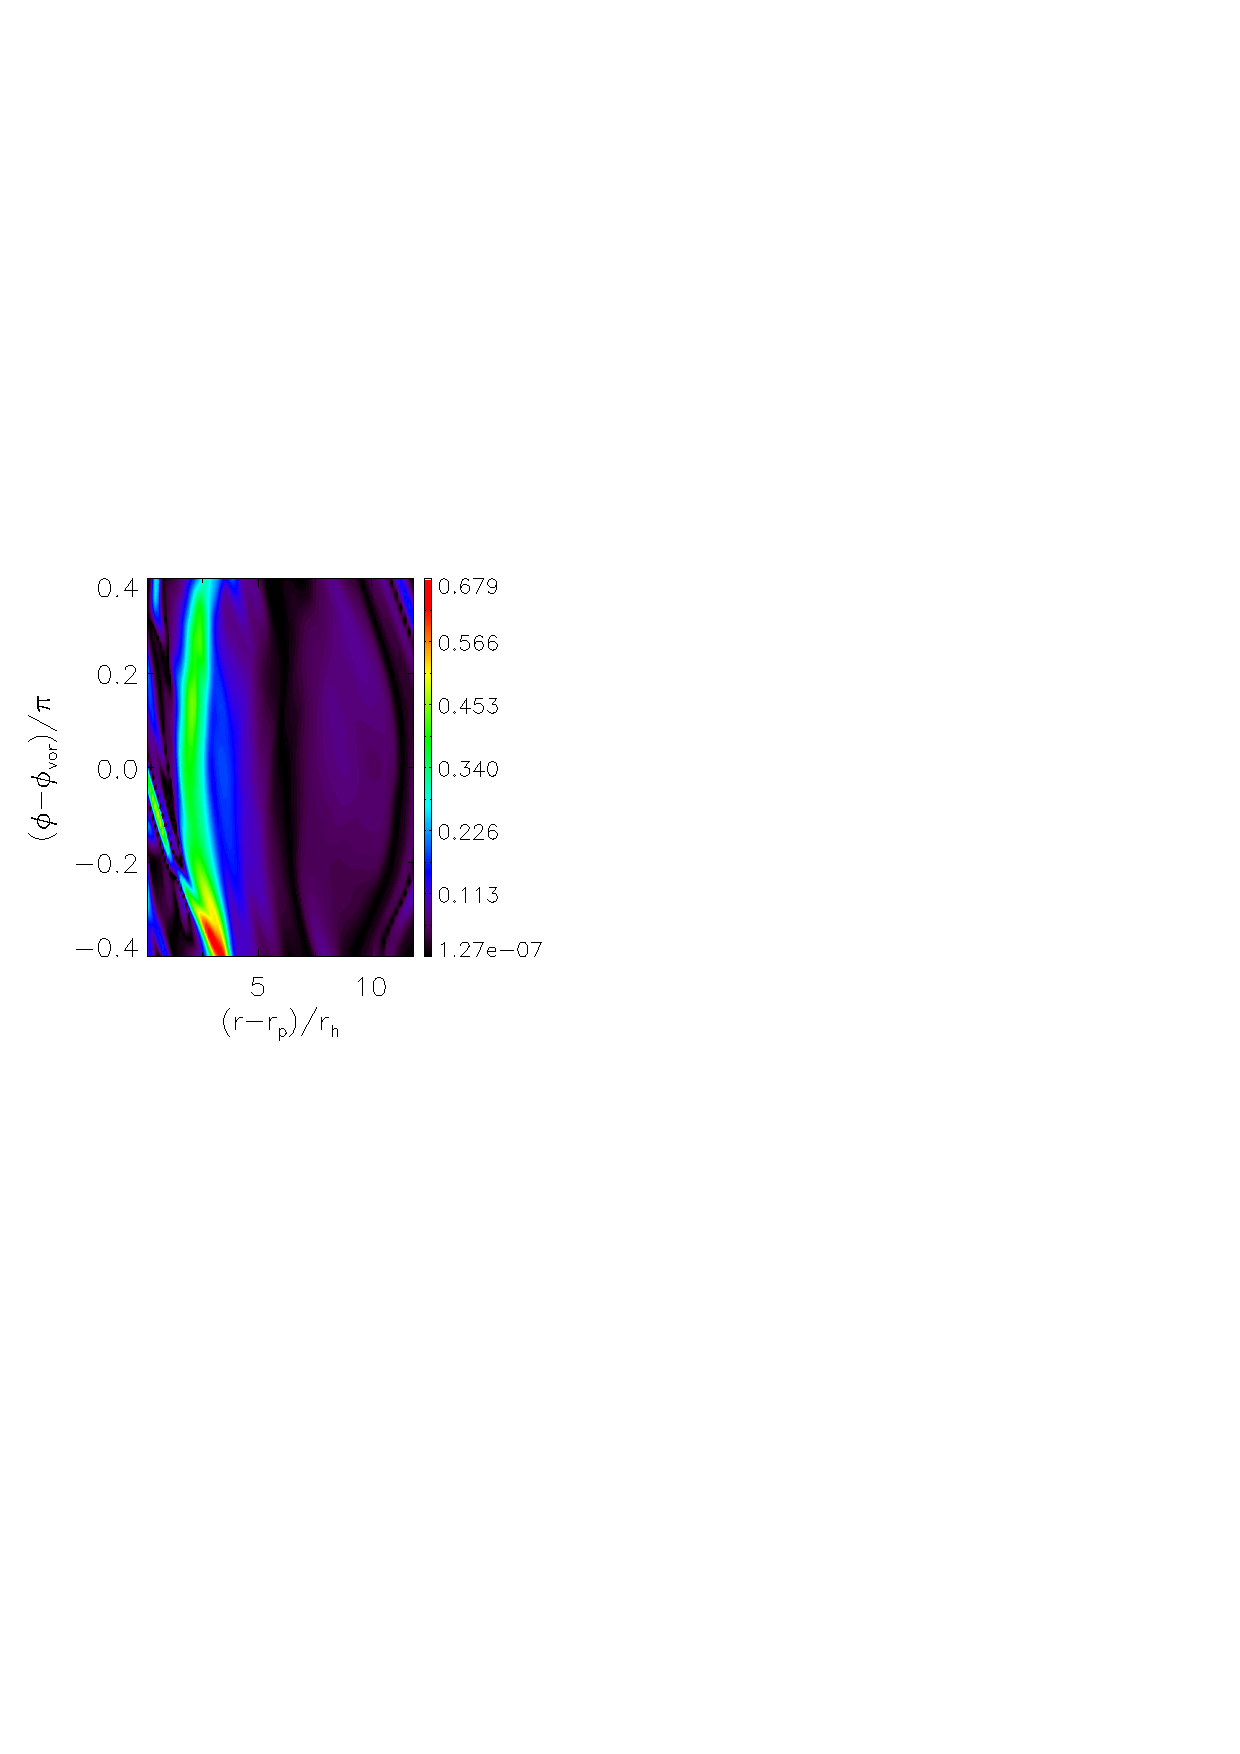
\includegraphics[width=0.3\linewidth]{figures/shock4}
  }
\hfill
  \subfigure{
    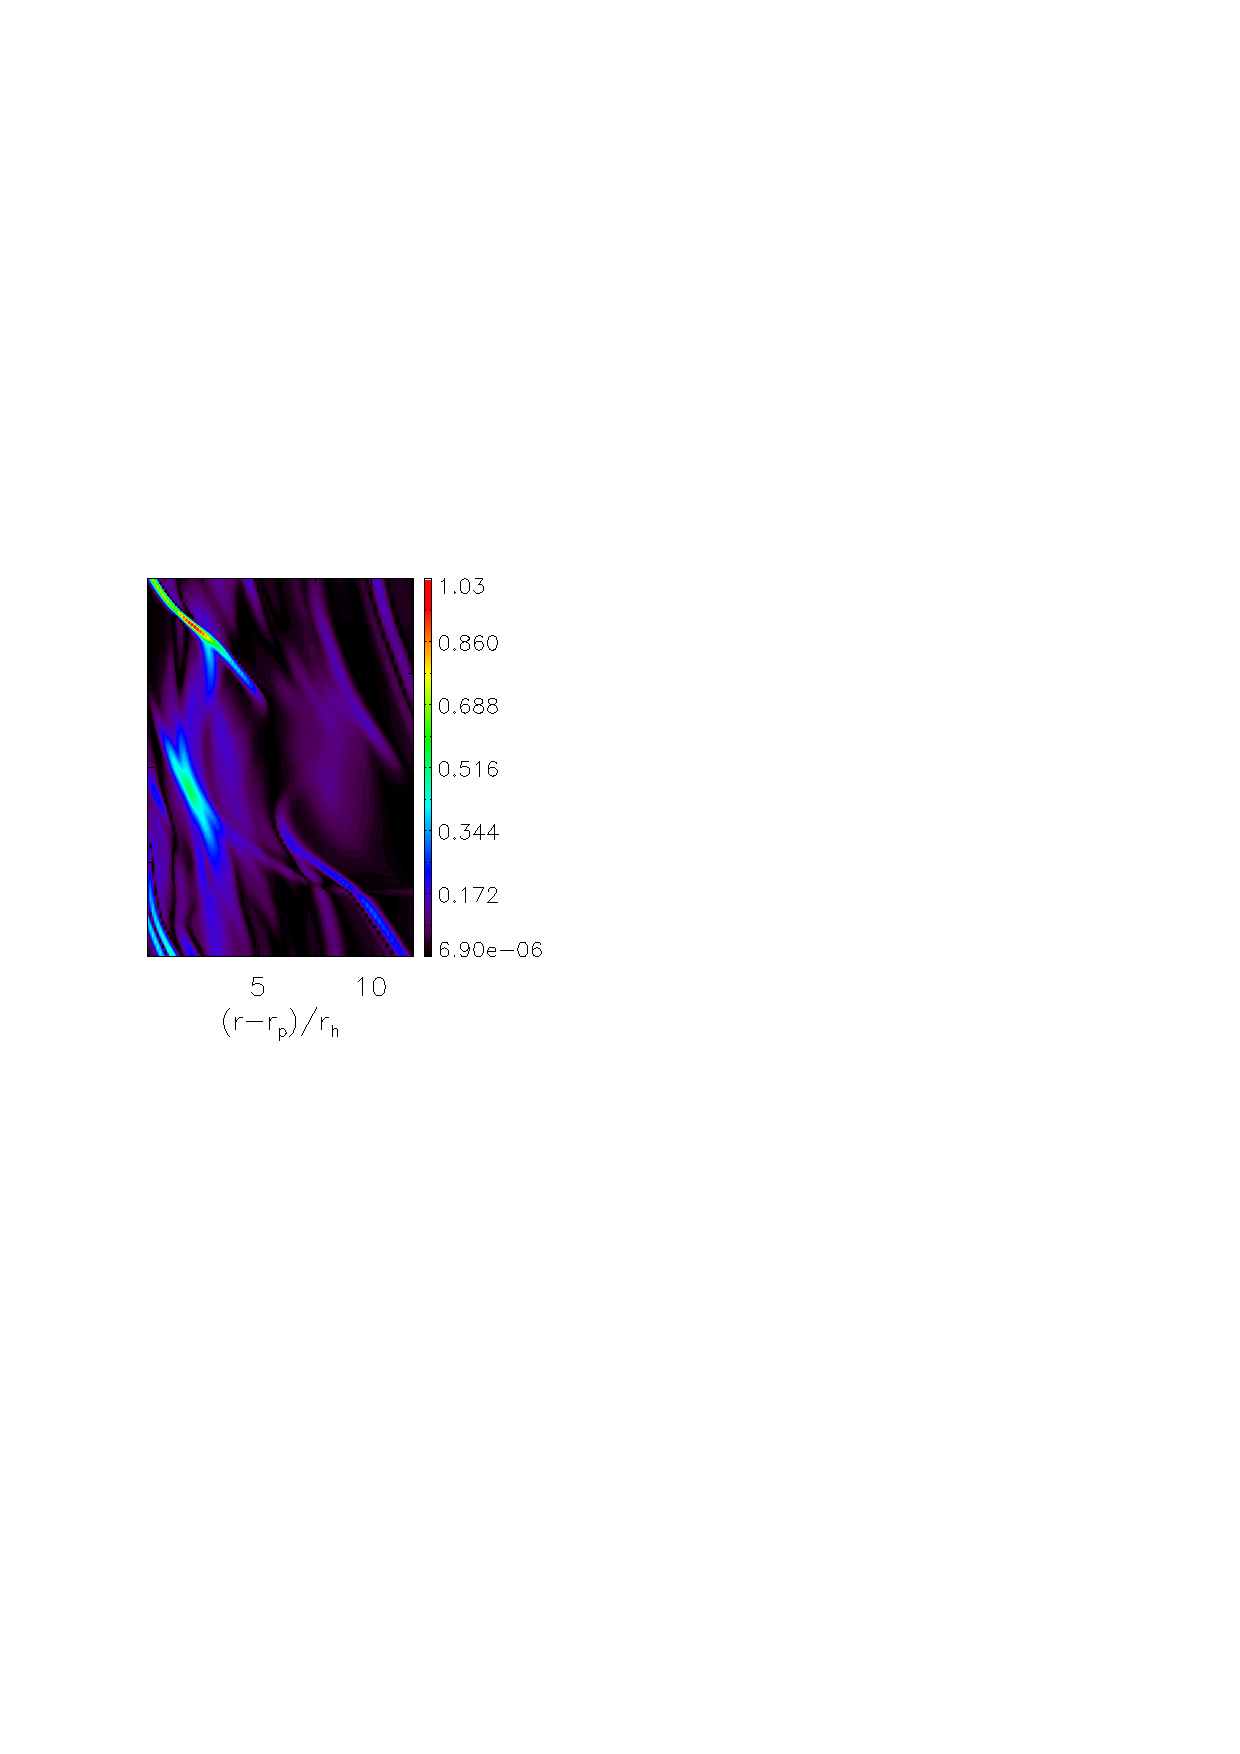
\includegraphics[width=0.3\linewidth]{figures/shock5}
  }
\hfill
  \subfigure{
    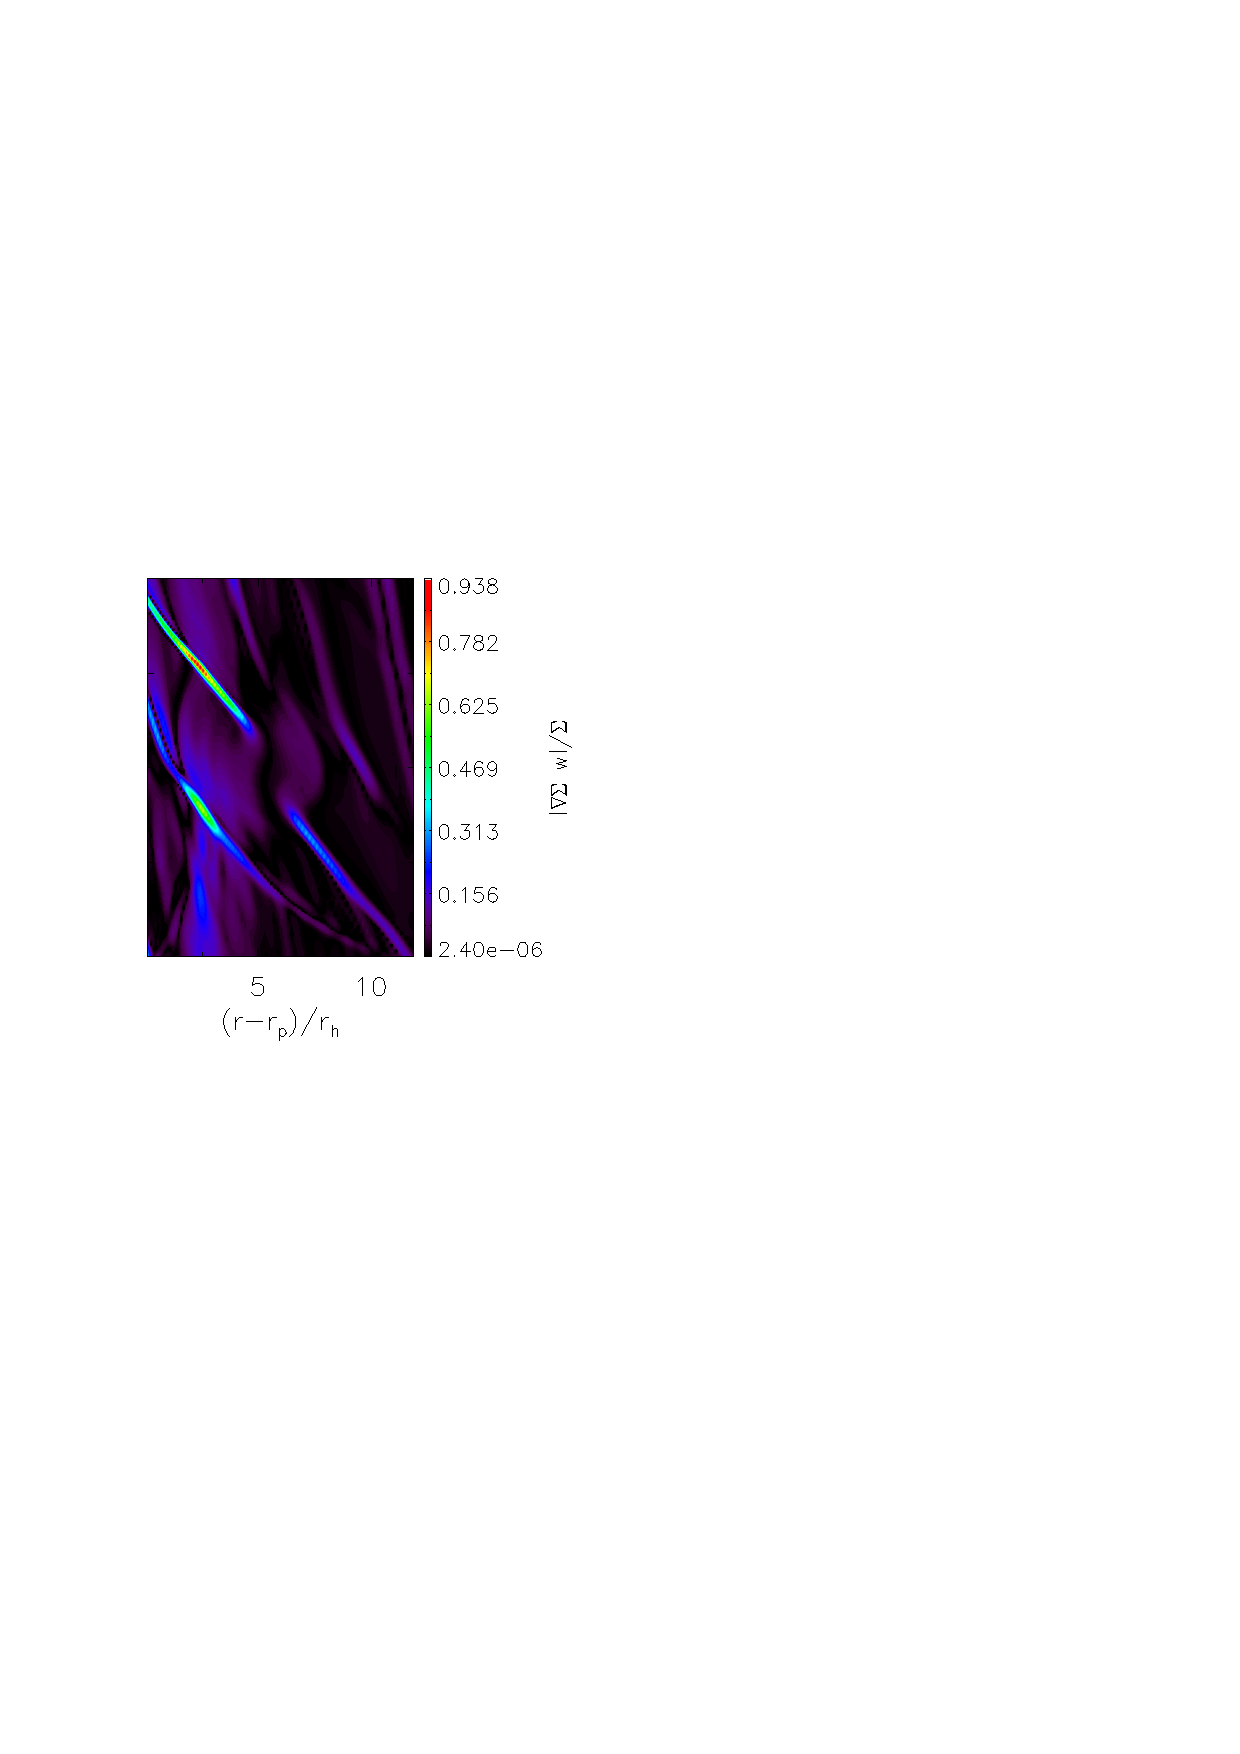
\includegraphics[width=0.3\linewidth]{figures/shock6}
  } 
  \caption{Evolution of the vortex in the case $\tilde{\beta}=1$
    just before its sudden decay. The surface density perturbation
    (top) and the associated surface density gradient (bottom) are shown.
    \label{shockplot}}
  % Large surface density gradients become prominant
  % around vortex during dissipation} 
\end{figure}

We also measured large increases in the Mach number near
the vortex when it begins to decay. Figure \ref{machplot} plots the
Mach number $M=|\bm{v} - \bm{v}_\mathrm{vor}|/c_s$, where
$\bm{v}_\mathrm{vor}$ corresponds to the bulk velocity of the vortex
around the disc. {\bf check - i assume this is the definition of mach
  number used here:yes this was the definition I used}. Values in Fig. \ref{machplot} have been averaged over
a region within $2H$ of the vortex centre.    
% Mach numbers with repect to the vortex bulk motion around the vortex
% region of $|r-r_{vortex}|<2H$
% are shown in  for various cooling rates over time.
During the quasi-steady state the Mach number increase
steadily, and for all cases $M$ reaches a maximum at 
% with larger growth rate for higher $\tilde\beta$.
a time coincident with the start of vortex decay.  

Putting the above observations together, we suggest the sudden decay
in the vortex amplitude is due to shock formation \emph{by the
  vortex}. When the vortex reaches large amplitude, it begins
to induce shocks in the surrounding fluid, as supported by the
increase in Mach number and the appearence of wakes with large surface
density gradients. The vortex may then lose energy through shock
dissipation. In addition, a strong vortex (or shock formation) 
also smoothes out the gap structure that originally gave rise to the
RWI, this would oppose vortex growth. We examine this below.

\begin{figure}
    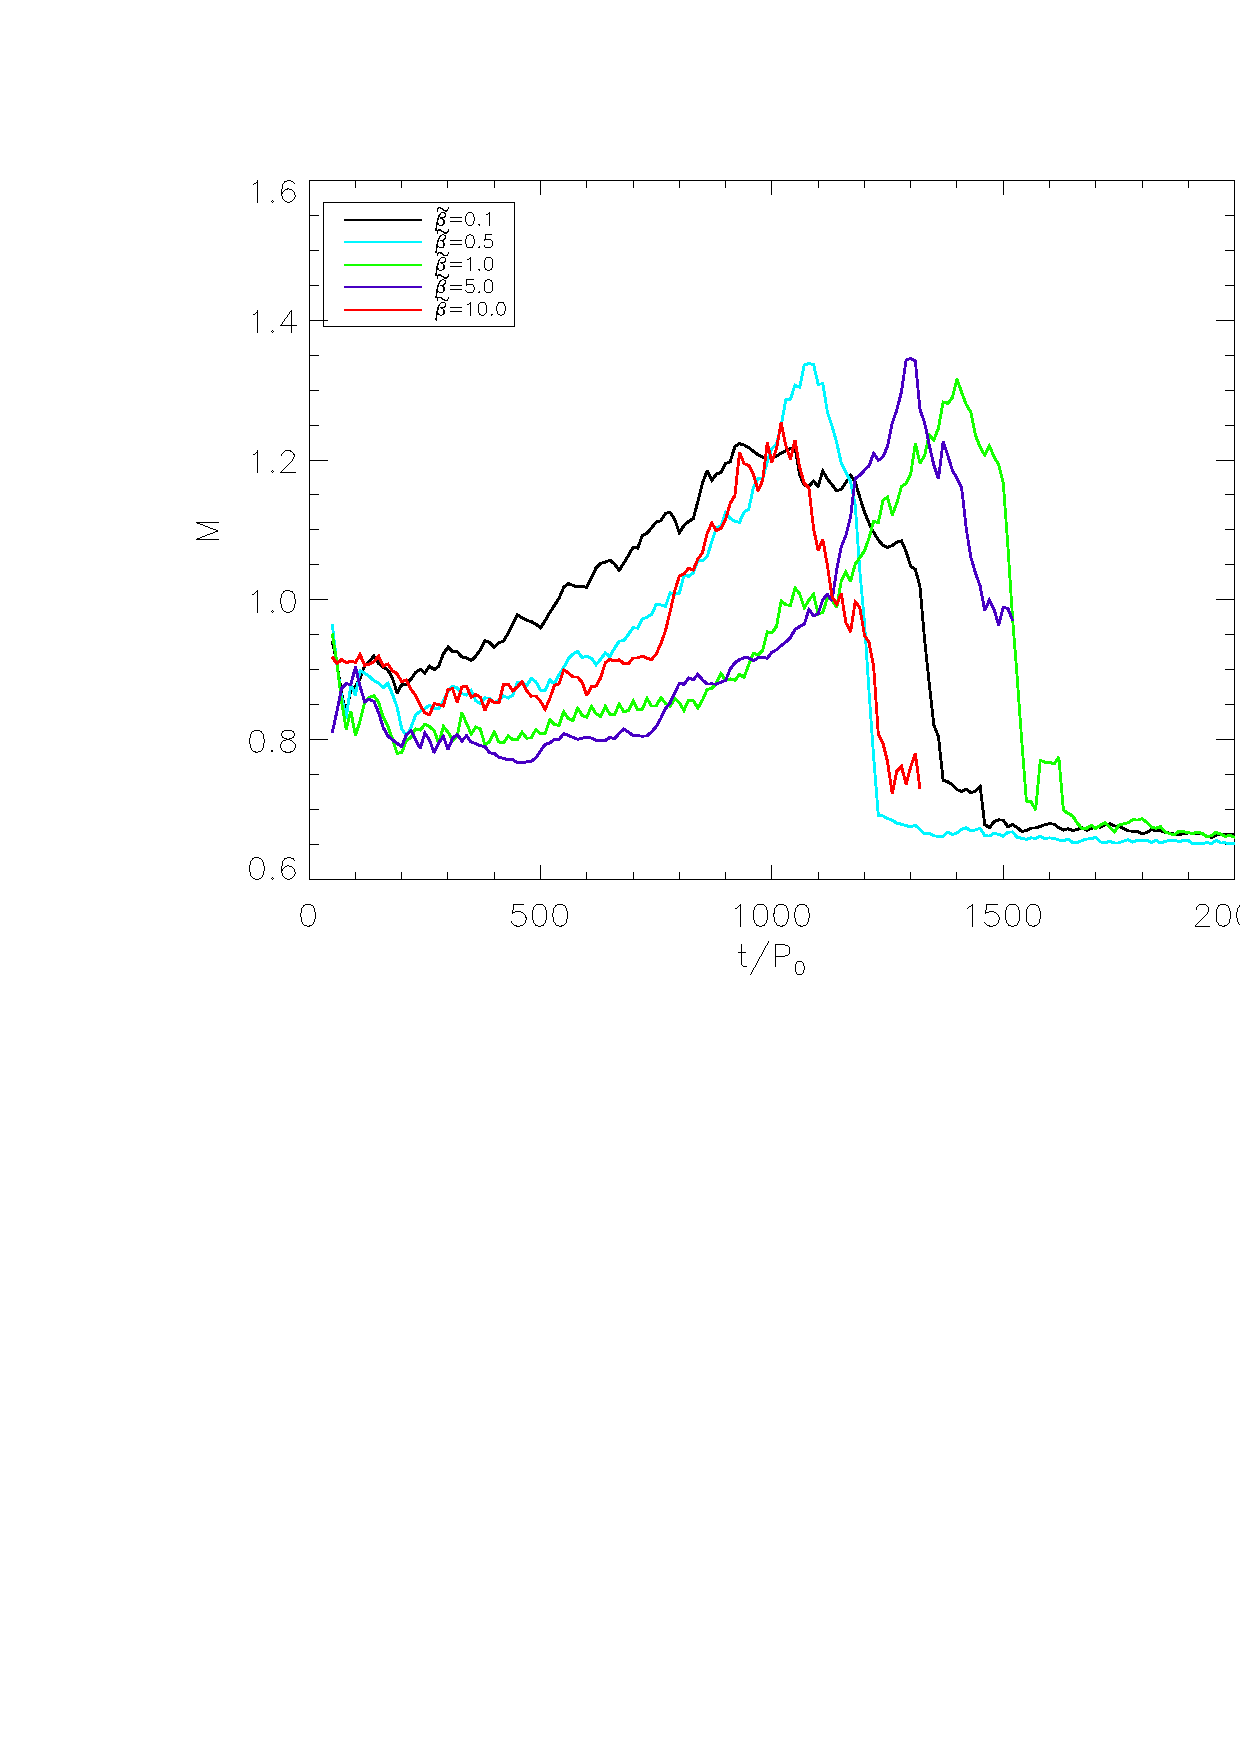
\includegraphics[width=\linewidth]{figures/mach}
 \caption{Running-time average {\bf ?} of the Mach number relative to
   the vortex, averaged over a region within $2H$ of the  
   vortex centre. This plot can be compared to the evolution of the
   vortex amplitude shown in Fig. \ref{lifetimeplot}.
   {\bf remember to update plot to include full simulation duration}
   \label{machplot}}
\end{figure}

\subsection{Effect of vortex dissipation on the gap structure} 
{\bf are these high resolution results?:yes}
We find vortex growth during the quasi-steady state and its dissipation
also modifies the gap structure. Here, we 
define a gap depth parameter by taking the azimuthal and radial average
of the relative surface density perturbation within $r\in[r_p,r_e]$ where
$r_{e}$ is defined as the outer gap radius such that 
$\langle\Delta \Sigma(r_e)/\Sigma(t=0)\rangle_{\phi}=0$. We are
interested in the region $r \in[r_p,r_e]$ since the vortex is
located at the outer gap edge. A more negative gap depth parameter
correlates with a steeper gap edge. 
{\bf notation clash: rout already used as outer disc boundary - choose
different notation. updated to $r_e$ for now}

Fig. \ref{gapdepth} shows the evolution of the gap depth parameter
for $\tilde\beta=1.0$. The magnitude of the gap depth is seen to 
slowly increase as vortex reaches its maximum amplutude at
$t=1000P_0$, followed by a sharp decrease coincident with vortex
dissipation.  

We see that the dissipation of the vortex has a `gap-filling'
effect, and we find that the gap edge is smoothed during this
process. This can be interpreted as the vortex providing a
viscosity, and we measure a typical alpha viscosity $\alpha = O(10^{-2})$
associated with the vortex. This acts against gap-opening
by the planet, and   
%The smoothening out of the gap edge during later half of quasi steady state
%is because the vortex has an associated viscosity $\alpha \sim O(10^{-2})$.
the condition for the RWI
becomes less favourable, which explains why vortices do not
reform again (at least within the simulation timescale).  

%The sudden smoothening of gap egde during dissipation is due to the large
%influx of density from the vortex to the gap.

\begin{figure}
  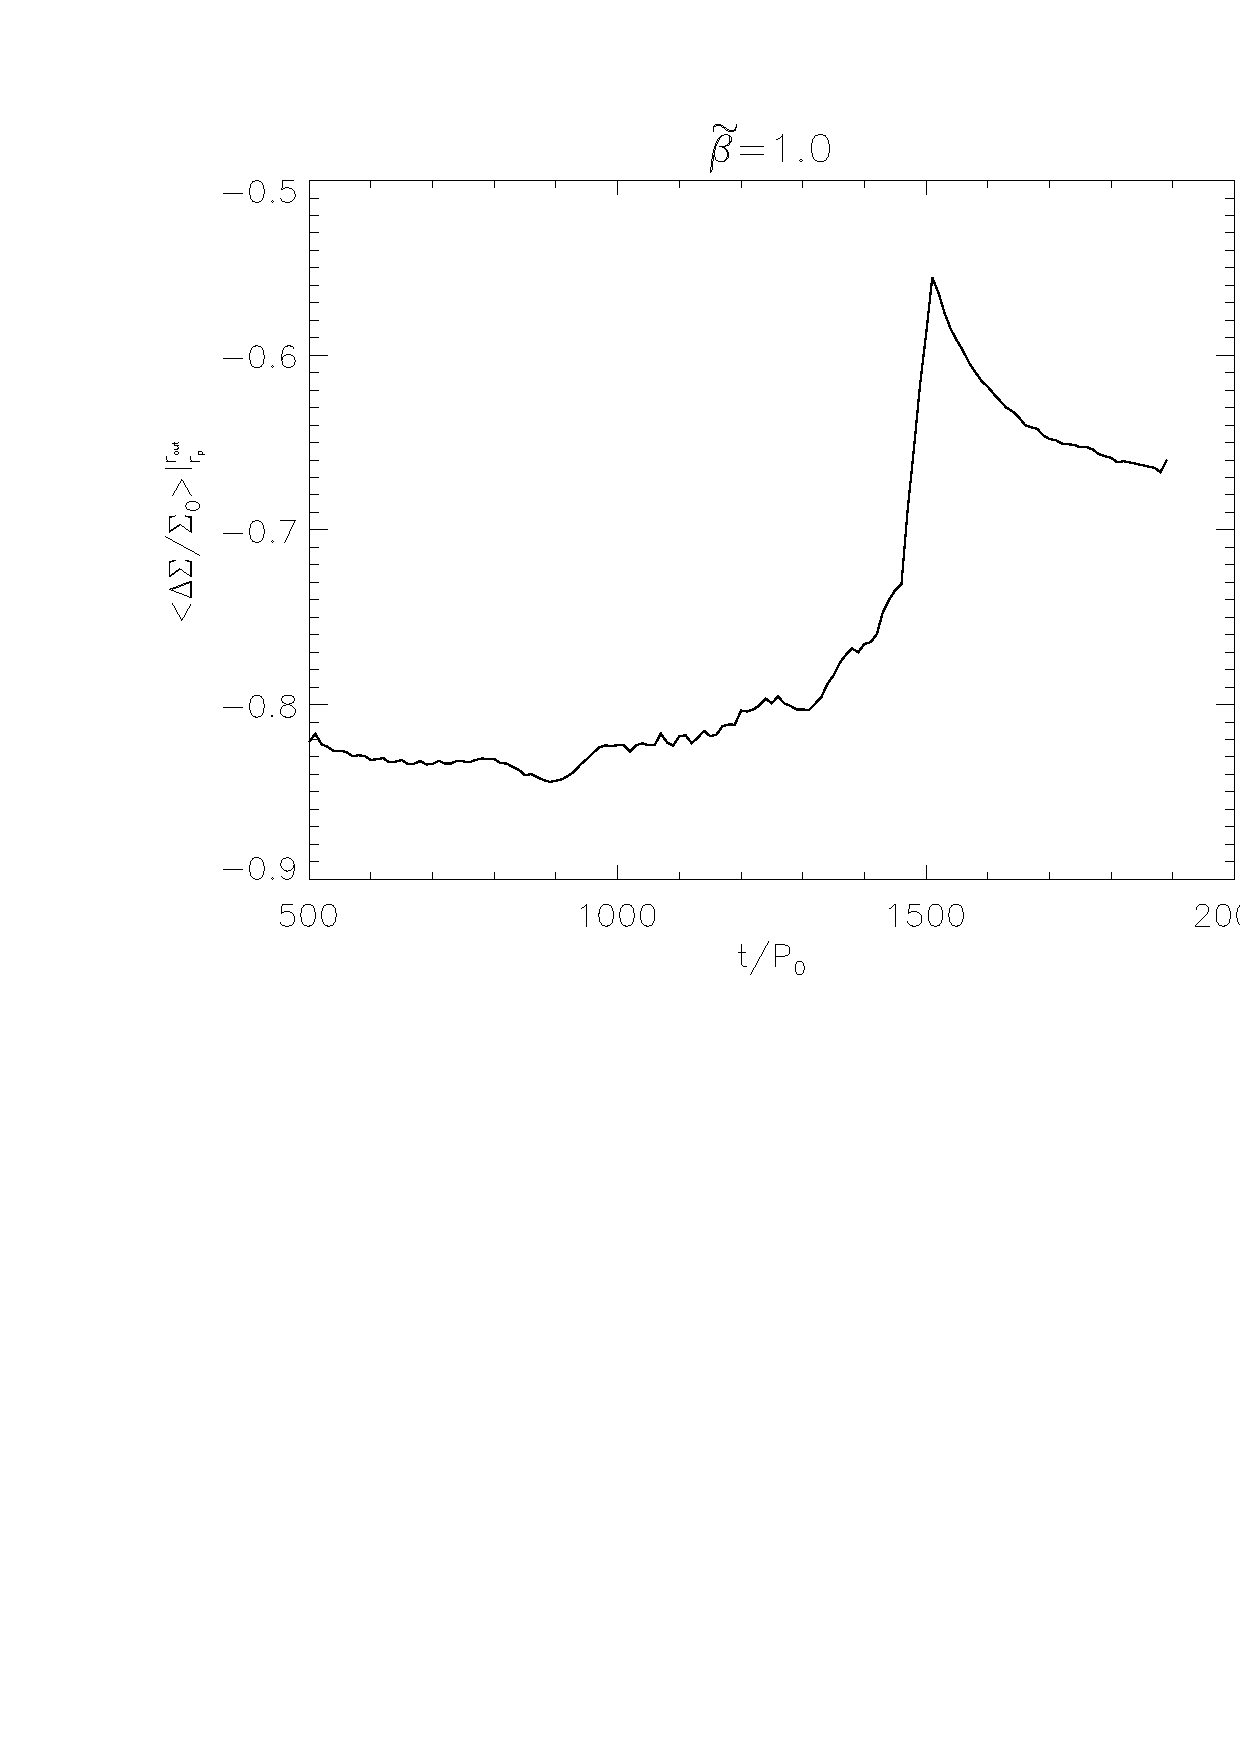
\includegraphics[width=\linewidth]{figures/gapdepth}
  \caption{Running-time average of the gap depth parameter, defined as
    the relative surface density perturbation averaged over the
    outer half of the gap.} \label{gapdepth}
\end{figure}

\begin{figure}
  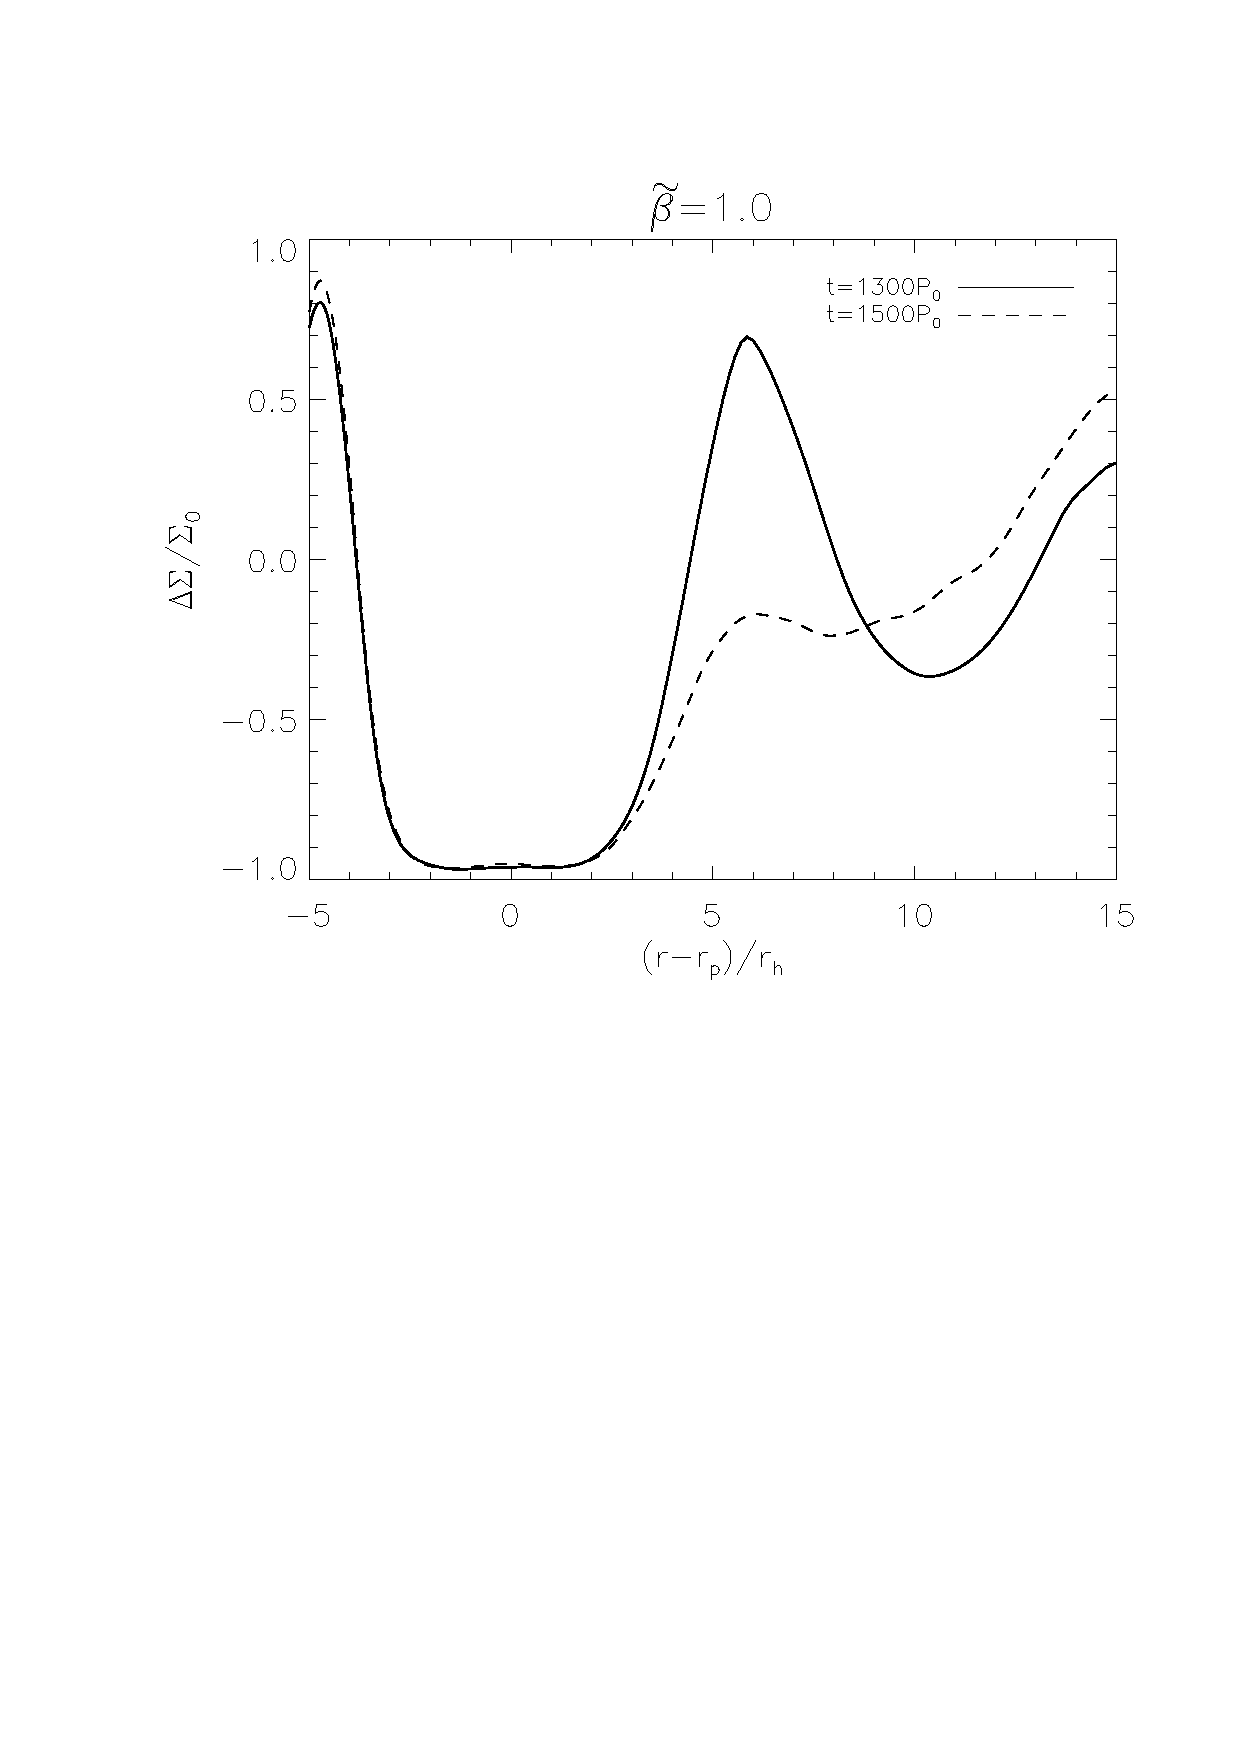
\includegraphics[width=\linewidth]{figures/gapchange}
  \caption{Azimuthally averaged gap profiles of relative surface change for
 before and after dissipation for $\tilde\beta=1.0$}
\end{figure}

\subsection{Vortex lifetimes as a function of cooling rate}

% {\bf describe dependency on
% cooling. Do we have enough data to have a `lifetime v.s. beta'
%   plot? here we want to explain why vortex lives longer with longer
%   cooling, but very long cooling results in shorter lifetimes. 
%   Consider the following quantities as a function of cooling:
%   initial strength of the single vortex; growth rate of single vortex
%   strength from its formation to just before death; ampiltude of
%   vortex just before death; disc temperature in the vortex region. 

%   we expect the initial $m=1$ vortex (after merging) to be weaker with
%   increasing cooling time because the instability is weaker. (see
%   meheut et al 2013, mnras, 430, 1988 who show that the initial vortex
%   amplitude after linear growth is correlated with the linear growth
%   rate). 

%   suppose the vortex shocks when it reaches a certain amplitude (which
%   probably increases with longer cooling rate because it's more
%   difficult to shock a hotter disc). as we
%   increase the cooling time, the initial $m=1$ vortex is weaker, it
%   also grows more slowly because gap-opening is opposed by a hotter
%   disc. the above implies that it takes longer for the vortex reach
%   the shock-inducing amplitude and dissipate.  

%   but the above is not consistent with non-monotonic behaviour, which
%   predicts the $\tilde{\beta}=10$ vortex to survive longest. this is
%   because we expect the initial vortex to be weakest (check) which
%   means it should take the longest to grow and shock. check
%   whether there's anything special about this case. one possibility is
%   that vortex growth during the quasi-steady state is actually faster
%   because of the raised temperature (li et al 2000 show increased
%   temperature favours RWI - possibiliy evidenced here by a stronger
%   vortex before death than other cases) 

%   perhaps have a case of $\tilde{\beta}=7.5$ as further evidence of
%   non-monotonic behaviour
% }

\begin{figure}
    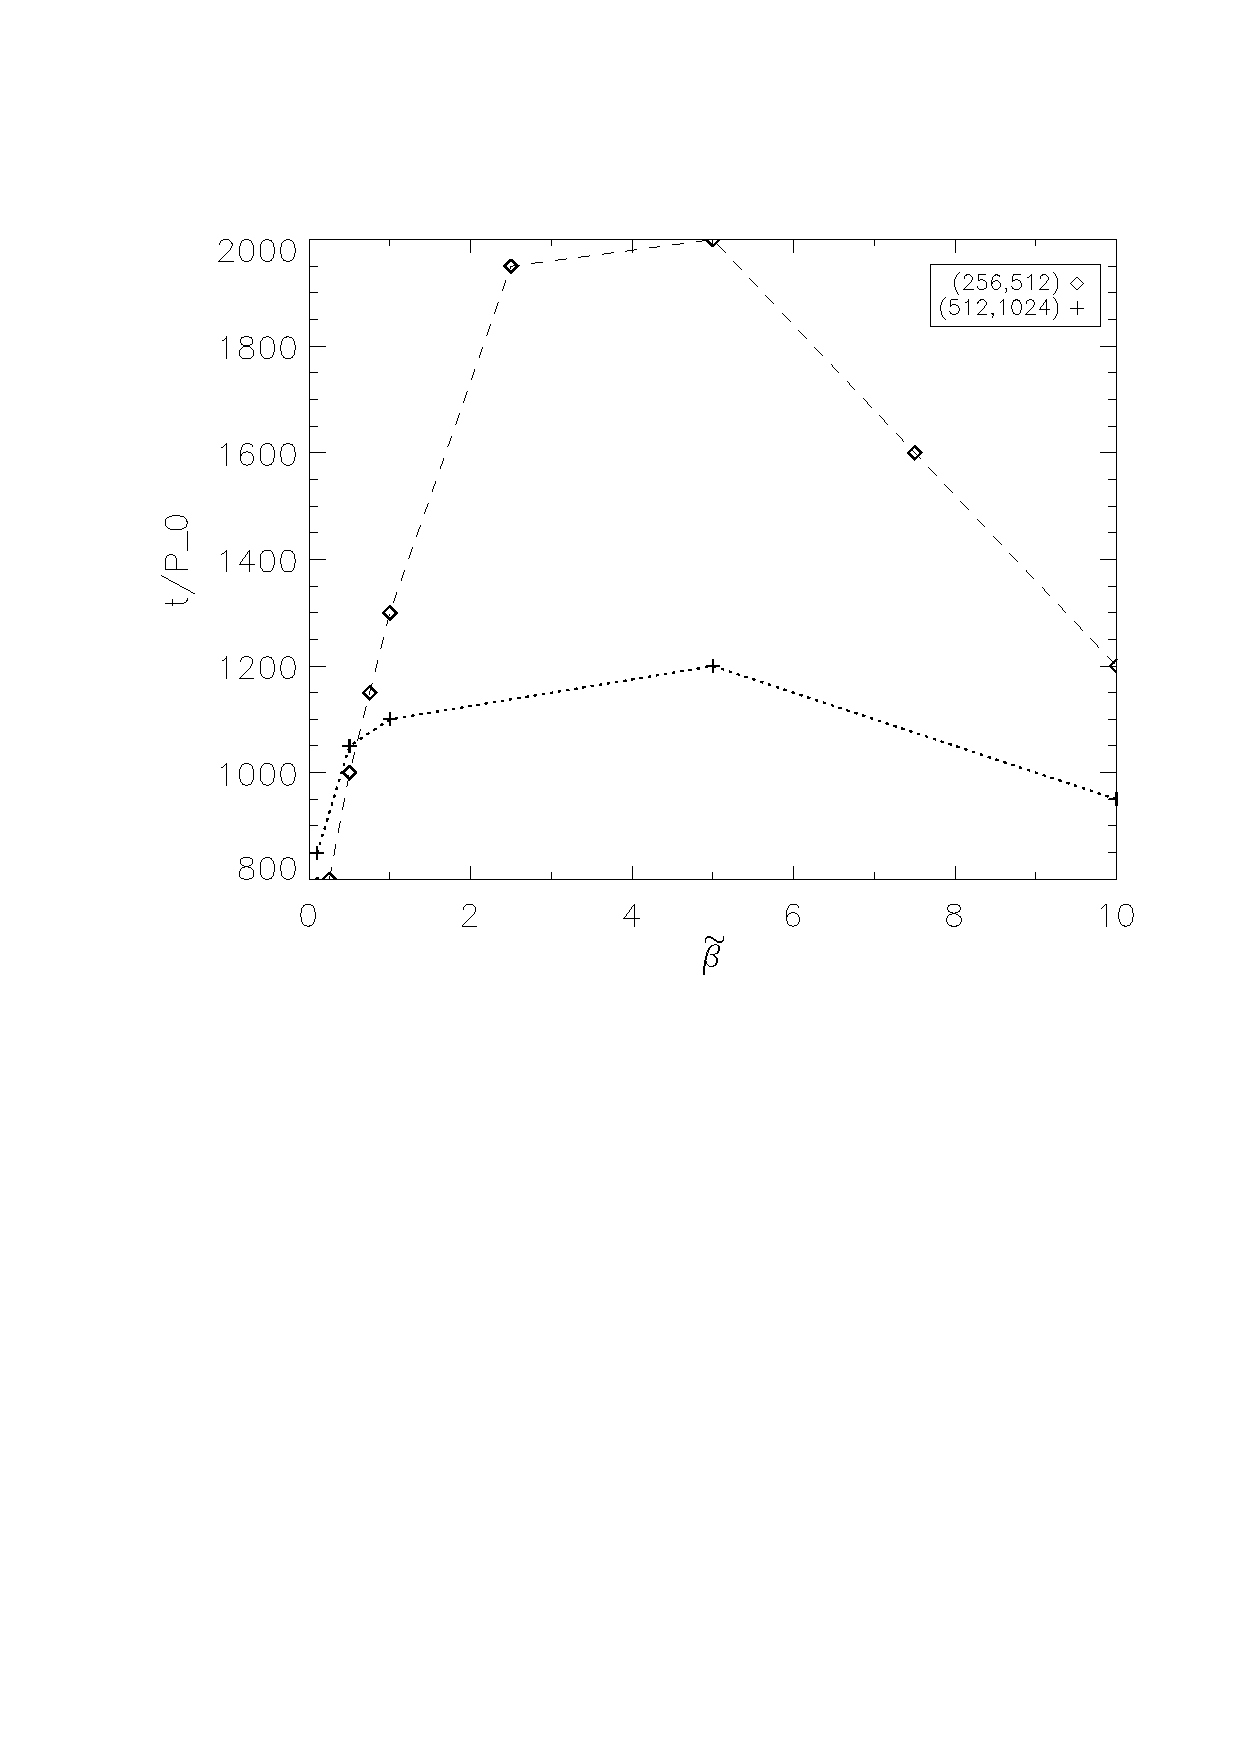
\includegraphics[width=\linewidth]{figures/betaplot}
 \caption{Lifetime of vortices with repect to cooling paramter $\tilde\beta$ for both resolution of $(N_r,N_\phi)=(256,512)$ and $(512,1024)${\bf update to high resolution results} } \label{betaplot}
\end{figure}

Fig. \ref{lifetimeplot} and Fig. \ref{betaplot} shows that increasing 
$\tilde{\beta}$
increases the lifetime of the vortex up to a critical 
value $\tilde{\beta}=5.0$ for which the vortex lasted to a simulation time of
 $1250P_0$ before starting to dissipate. This is consistent in time with the
 vortex introducing shocks to the system.

Our `planet-off' simulations
indicate weaker vortices are formed initially with increased cooling
times. This is because it has been shown that vortex amplitude is dependent on 
growth rate of the linear modes \citep{meheut2013}.
At the beginning of the vortex quasi-steady state $t=100P_0$ we find
that the relative surface density boost at center of vortex 
is $\Delta\Sigma/\Sigma_0=2.5$ for $\tilde\beta=0.1$ 
and decreases down to a minimum value of $\Delta\Sigma/\Sigma_0=1.48$ for 
$\tilde\beta=10$. 

 After merging, the growth of the single vortex, mediated by disc-planet
interaction, is expected to be slower with increased cooling time
because gap-opening becomes more difficult in a hotter
disc. Furthermore, the increased sound-speed suggest the vortex should
reach larger amplitudes in order to induce shocks. 
These expectations
imply that it takes longer for the vortex to induce shocks and
dissipate, and hence longer lifetimes with increasing
$\tilde{\beta}$. 

However, Fig. \ref{lifetimeplot} shows that increasing the cooling
time further to $\tilde{\beta}=10$ actually results in a
\emph{shorter} vortex lifetime. Notice for $\tilde{\beta}=10$ the vortex growth 
during the quasi-steady state is faster than for
$\tilde{\beta}=5$.
 This may be attributed to the higher temperature
reached in the latter case ($h\simeq 0.07$) in comparison with the former
($h\simeq 0.06$)
% {\bf temperature for $\tilde{\beta}=5$?}
, since \cite{li00} showed that the RWI grows
faster with increased disc temperature. At long cooling times, this
effect may dominate over the weaker gap-opening effect at higher $h$.   

This effect can be seen in Mach number around the vortices where the
growth of Mach number with respect to time is increasing with cooling rate.
Thus the intially weaker formed vortices for higher cooling rate grow
substantialy faster than the sound speed and can shock the system in earlier
times.

Thus, unlike our `planet-off' simulations we find that there is
a cooling time $t_c$ which maximises the vortex lifetime. In the long term
 'planet-off' simulations we find that the vortices dissipate very gradually
 and visciously dependent on cooling rate.
% {\bf to make this comparison we need to discuss vortex lifetimes for planet-offsimulations as well} 
This
non-monotonic behaviour was also reported by \cite{fu14}, who
performed isothermal disc-planet simluations with different fixed
aspectratios.   
%Cooling rates with
%$\tilde\beta>5.0$ showed lifetimes that were well below the max
%lifetime. 
By analyzing the radial region around the vortex within
 $[2r_{h},10r_{h}]$
% {\bf define this region}
 we find the
$\tilde\beta=5.0$ case, with the longest vortex lifetime, has
$h\approx0.06$ on average throughout its lifetime. This value of $h$ was also
 found to maximize vortex
lifetimes in the isothermal simulations of \cite{fu14}. Note that $h$ is a fixed
quantity in \cite{fu14} while in this work $h$ is a dynamical variable dependent
 on the viscous heating and cooling rate as by choice of energy equation.

These results were reproduced in lower resolution simulations as well. Vortex
shocks were similarly seen during vortex dissipation and non-monotonic
 dependence on lifetime with $\tilde\beta$ was similarly found.
Vortex lifetimes are considerably longer in these runs with the maximum
 lifetime longer than the simulation timescale of $2000P_o$ for 
$\tilde\beta=5.0$ which again has $h\approx0.06$.
This inconsistancy in timescales, may be due to resolution as a finer 
grid spacing is required to accurately
reproduce jump conditions along shocks and which cause vortex dissipation.
 {\bf this is the best reason I could personally think of, for lower
   beta runs vortices last slightly longer but for higher values it is
   quite drasticly different. Not sure how numerical dissipation as
   you mentioned would be a factor in this case} 
{\bf you mentioned resolution and convergence to me being a known issue in a previous email}

%be the optimum lifetime for long-term simulations of
%isothermal disks with varying intial temperature profiles $h$. 

%Competing effects of gap stability with $t_{\mathrm{coo}l}$ result in
%the the non-montonic form of the lifetime. As the $\tilde\beta$
%increases so does the stability of the gap edge as seen in
%section~\ref{linear}, however as $\tilde\beta$ increases so does the
%$c_{\mathrm{iso}}$ which is known from theory to effect the growth of
%instability \citep{li00}. Thus increasing $\tilde\beta$ increases the
%sound speed $c_{\mathrm{iso}}$ and likewise the gap instability up to
%a certain point in which the effects of the more stable gap edge
%becomes a significant effect. 

%The correlation of growth rate and sound
%speed is non-negligible as in previous `planet-off' case as the disk
%now can reach values of $h\simeq0.08$ for very slow cooling and the
%importance of the effect can be imagined to accumulate over the now
%considerably longer timescale. These effects dictate when then the
%vortex reaches the critical value in which it shocks the system that
%subsequently causes disspation and hence the lifetime fo the vortex. 







%\section{Additional results analysis}\label{additional}
In this section we examine some secondary quantities derived
from the hydrodynamic simulations above. To keep this discussion
concise, we will use selected simulations from above for illustration.   

\subsection{Three-dimensionality}
A simple measure of three-dimensionality of the flow is to compare vertical 
to horizontal motion. Since we are interested in non-axisymmetric
perturbations to the gap edge, we first Fourier transform the
meridional momentum densities 

\begin{align}
  (v_{Rm}, v_{zm} ) \equiv\int_0^{2\pi}\rho\times(u_R,
  u_z)\exp{(-\ii m\phi)}d\phi. 
\end{align}
We define the three dimensionality as $\Theta_m(z/H)$, where 
\begin{align}
  \Theta_m^2 \equiv \frac{\avg{|v_{zm}|^2}}{\avg{|v_{zm}|^2}
    +\avg{|v_{Rm}|^2}},  
\end{align}
and $\avg{\cdot}$ denotes a radial average. 
Admittedly, this is a crude measure, and exact values of $\Theta_m$
varies somewhat with details of the average. However, we have
experimented with different averaging domains and 
found the features described below are robust.  


The top panel in Fig. \ref{compare_vprofiles_3d008} shows $\Theta_m$
for Cases 1--3 at $t=40P_0$. The radial average is taken over
$r-r_p\in[3,7]r_h$. These are all vortex modes (see
Fig. \ref{vortex8_polar_dens} and
Fig. \ref{vortex4_vortex10_overall}). The flow becomes increasingly
three-dimensional away from the midplane but 
$\Theta_m = O(10^{-1})$ is small. In an averaged sense the flow is
mostly horizontal. At the end of the  
simulation for Case 1, an azimuthally extended vortex dominates the
flow, for which we measured $\Theta_1\sim
0.2$---0.3. Thus, although vertical motion can become an appreciable
fraction of horizontal motion, the former never dominates.  

$\Theta_m$ for Cases 4---7 are shown in in bottom panel of
Fig. \ref{compare_vprofiles_3d008}. The radial average is performed
over $r-r_p\in[2,6]r_h$ 
because the global spirals in Cases 6---7 significantly protrude the
gap edge. The snapshot is taken at $t=50P_0$ for Cases 4---5, at
$t=40P_0$ for Case 6 and at $t=30P_0$, so that the
vortices and spirals have comparable over-densities at the
gap edge. It also reflects the fact that spiral modes are more
unstable than vortex modes and develop earlier  
\citep{lin11b}. $\Theta_m \sim 0.2$ is again not particularly
large, but the spiral modes are distinctly more three-dimensional than
vortex modes. This is likely due to additional vertical
acceleration provided by the strong self-gravity in those cases.   


%
% can't do detail comparision between cases because instability have
% different growth rates. different 'stages' in instability

% Case 6 show 3 edge disturbances but this is likely to be a mixture
% of spiral and vortex modes, rather than the m=3 spiral mode. This is
% because 
% we clearly see m=2 spiral in Case 7 (Q_0=1.5), and to see higher m spiral
% modes one should increase the strength of self-gravity (e.g. lin11b
% observe m=3 spirals with Q_0=1.2) 
%

\begin{figure}
  \centering
  \includegraphics[scale=.425,clip=true,trim=0.2cm 1.7cm 0cm
    0cm]{figures/compare_vprofiles_3d008}  
  \includegraphics[scale=.425,clip=true,trim=0.2cm 0cm 0cm
    0.2cm]{figures/compare_vprofiles_3d010}  
  \caption{Three-dimensionality of the non-axisymmetric
    flow near the outer gap edge. Top: Cases 1---3 (vortex modes). 
    Bottom: Cases 4---5 (vortex modes) and Cases 6---7 (spiral
    modes). The azimuthal wavenumber $m$ is chosen to match the number
    of vortices or large-scale spirals observed. 
    \label{compare_vprofiles_3d008}}
\end{figure}

\subsection{Vortensity field}\label{vortensity}
A fundamental distinction between the linear vortex and edge mode
instability is their association with local vortensity minimum and
maximum, respectively. In this section we compare vortensity fields of 
discs with vortex modes (Case 2) and edge modes (Case 7). 
%We use Case 2 
%and Case 7 as examples, respectively. 
More specifically, we examine the relative
perturbation to the vertical component of vortensity,  
\begin{align}
  \Delta\eta_z\equiv \frac{\eta_z - \eta_z(t=0)}{\eta_z(t=0)},
\end{align}
where
\begin{align}
  \eta_z \equiv \frac{\bm{\hat{z}}\cdot\nabla\times\bm{u}}{\rho}. 
\end{align}

Fig. \ref{vortex4_vortex1_vortxy} compares $\Delta\eta_z$ in the
midplane when vortices and spirals develop. For planetary gaps, 
vortensity maxima and minima are both located near the gap edges with 
characteristic separation of the local scale-height. The vortensity
ring at the inner gap edge ($r-r_p\simeq - 2r_h$) remain
well-defined. The vortex instability is associated with the local
vortensity minimum near the outer gap edge --- seen as localised closed
contour lines centred about $r - r_p \sim 4r_h$. The vortensity ring at
$r-r_p\sim +2r_h$ becomes distorted as a \emph{consequence} of
large-scale vortex formation just exterior to it. By contrast, the
edge-spiral mode is associated with the local vortensity
maximum. Their development inherently disrupts the vortensity
rings. This is seen in the right panel as the outer ring is broken up.    
    
\begin{figure}
  \centering
  \includegraphics[scale=.425,clip=true,trim=0cm 0cm 1.9cm 
    0.9cm]{figures/vortex4_vortxy_008}\includegraphics[scale=.425,clip=true,trim=2.3cm    
    0.0cm 0cm 
    0.9cm]{figures/vortex1_vortxy_006}
  \caption{Relative perturbation to the vertical component of
    vortensity at the midplane in a disc with the vortex instability
    (left, Case 2 at $t=40P_0$) and the 
    spiral instability (right, Case 7 at $t=30P_0$). Negative
    perturbations in the region $r-r_p\in[2,6]r_h$ are outlined by white lines. 
    Dotted horizontal lines indicate azimuthal cuts taken in
    Fig. \ref{vortex4_vortex1_vortRZ}.   
    \label{vortex4_vortex1_vortxy}}
\end{figure}


The vertical structures also differ. Fig. \ref{vortex4_vortex1_vortRZ}
compares $\Delta\eta_z$ at azimuths coinciding with 
a vortex or the edge disturbance of the spiral mode. Both
instabilities involve $\Delta\eta_z<0$. It is clear that 
the spiral mode has stronger vertical dependence. Its 
region of $\Delta\eta_z<0$ becomes thinner away from
the midplane. In the vortex case this region remains 
about the same width and  $\Delta\eta_z$ is approximately uniform
within it. 
%This is qualitatively
%consistent with increased (downards) vertical motion. 
While $\mathrm{min}(\Delta\eta_z)$ is of comparable
magnitude, the vortensity ring at $r-r_p=2r_h$is much weaker and
thinner in the spiral case ($\Delta\eta_z$ being a factor $\sim 4$
smaller than the vortex case).   
 

\begin{figure}
  \centering
  \includegraphics[scale=.47,clip=true,trim=0cm 1.32cm .0cm
    .6cm]{figures/vortex4_vortRZ_008}\\\includegraphics[scale=.47,clip=true,trim=0cm 
    0.cm .0cm
    .6cm]{figures/vortex1_vortRZ_006}
  \caption{Relative vertical vortensity perturbation
    associated with the vortex instability (top) and spiral
    instability (bottom). The slices are taken at azimuths shown by
    white dotted lines in Fig. \ref{vortex4_vortex1_vortxy}. Negative
    perturbations in the region $r-r_p\in[2,5.5]r_h$ are outlined by
    white lines. \label{vortex4_vortex1_vortRZ}} 
\end{figure}

\subsection{Disc-planet torques}
The presence of non-axisymmetric disturbances at gap edges is
expected to significantly affect disc-planet torques. It has been 
confirmed in 2D simulations that both vortex and spiral modes lead to
oscillatory torques of either sign \citep{li05,lin11b}. 
%Limited 
%numerical resolution the current 3D calculations prevent accurate torque measurements, 
It this section we measure the disc-on-planet torques in several of the above simulations
to confirm the main features found in 2D. 

We calculate the specific torque acting on the planet due to a mass
element as 
\begin{align}
d\bm{T}(\bm{r}) &=
\frac{\bm{r}_p\times\bm{r}G\rho(\bm{r})d^3\bm{r}}{d_p^3}f(\bm{r},\bm{r}_p),\\
f(\bm{r},\bm{r}_p)&\equiv 1
-\exp{\left(-\frac{1}{2}\left|\frac{\bm{r}-\bm{r}_p}{\epsilon_c
      r_h}\right|^2\right)}.  
\end{align} 
The tapering function $f$ reduce contributions from close to the
planet, thereby reducing numerical artifacts arising from this region
because of the diverging potential and limited resolution. We set  
the parameter $\epsilon_c=1$ so that tapering does not significantly
reduce contributions from the instabilities, since they develop
at $\gtrsim 2r_h$ away from the planet's orbital radius.  

Fig. \ref{torque3} shows the disc-on-planet torques in Case 3 and Case 5, which develop
the $m=5$ and $m=6$ vortex modes, respectively. These plots are qualitatively similar to
2D simulations \citep[e.g.][]{li05}. The torques oscillate on orbital 
time-scales and its instantaneous values can be of either sign. However, 
upon averaging over the simulation we find the total torques are negative in both cases. This
means inwards migration is still favoured. 
%The planet is expected to interact

We extended Case 5 to $t=135P_0$ and find the vortices 
have similar over-densities as at $t=50P_0$. However, 
Fig. \ref{torque3} show the torque oscillation amplitudes decrease
towards the end of Case 5 compared to $t\in[40,80]P_0$.  
At $t=50P_0$ the vortices are located in $r-r_p\in[3.5,5.5]r_h$ but by
$t=135P_0$ they are located in $r-r_p\in[4,6]r_h$. 
Given that $t\in[40,80]P_0$ is only $20P_0$ to $50P_0$ after the planet  
potential has been fully introduced, gap-formation is probably 
ongoing during this time. We expect torque amplitudes to be larger
during  gap-formation since the vortices lie closer to the planet. 
%On the
%other hand, gap-widening in the presence of vortices was also seen in  
%2D simulations on long timescales \citep{lin11a}  
%So there may also be
%contributions from radial redistribution of material due to the
%vortices. 
% This might be
%brought about by the of the density bump at the outer gap edge
%\citep{meheut12b}  


%The original
%density bump at the outer gap edge ($r-r_p\simeq 4r_h$) shifts outward
%between these times. 
%This is unlike in the fixed-orbit 2D simulation by \cite{li05}, where
%the oscillation amplitude does not decrease over several hundred
%orbits. 
%The different setups (especially self-gravity and numerical resolution) 
%prevent a detail comparison 
roclinic instability
 
\begin{figure}
  \centering
  \includegraphics[scale=.425,clip=true,trim=0.2cm 1.cm 0cm
    0cm]{figures/vortex10_torque3_tqex}  
  \includegraphics[scale=.425,clip=true,trim=0.2cm 0cm 0cm 0.2cm]{figures/vortex2b_torque3_tqex} 
  \caption{Instantaneous disc-on-planet torques in simulations where the vortex mode develops. 
    Top: Case 3. Bottom: Case 5. Note that Case 5 has been extended to $t=135P_0$. \label{torque3}}
\end{figure}

Next we examine disc-planet torques in the presence of the spiral
modes. The top panel of Fig. \ref{torque3_spiral} shows the
instantaneous disc-on-planet torques. Contributions from the
inner disc ($r < r_p$) and outer disc ($r > r_p$) are plotted
separately for comparison with Fig. 18b in \cite{lin11b}, which is 
similar to the present plot. Large oscillations in the outer torque
due to edge mode spirals cause the total torque to be positive or
negative at a given instant. 

Unlike the vortex modes, Fig. \ref{torque3_spiral} shows that spiral
modes can lead to a positive running-time averaged torques (bottom panel). 
The average torques become more positive with time after spiral modes develop, 
and with increasing self-gravity (which increases the instability strength). 
%The torque is more positive with
%increasing strength of the spiral instability.
This was also observed in high-resolution 2D simulations in
\cite{lin11b}. There it was suggested that the creation of large   
`voids' in between spiral arms decreases the time-averaged density in  
the planet-induced wakes, thereby reducing associated torque
magnitudes. Since the outer planetary wake normally provide a negative
torque, the spiral modes make the total torque more positive. 
The similarity between 2D and 3D results indicate that
outwards migration induced by spiral modes, which was seen in 2D by
\cite{lin11b,lin12b}, will also operate in 3D.      

%It was later shown that the spiral instability can supply material to
%go on horseshoe turns ahead of the planet, which also provide a
%positive torque \citep{lin12b}. This is because the spiral modes 
%are associated with local vortensity maximum which are located just
%inside the gap edge in the co-orbital region. 

%This is because the
%spirals are associated with local vortensity maximum, which is just
%inside the outer gap edge. Thus over-densities can be supplied by the
%instability to go on horseshoe orbits

%Since spiral modes are associated with disturbances at the local
%vortensity maximum just inside the outer gap edge, its influence on
%disc-planet torques is expected to be more si

\begin{figure}
  \centering
  \includegraphics[scale=.425,clip=true,trim=0.2cm 1.825cm 0cm
    0cm]{figures/vortex1_torque2_tqex}  
  \includegraphics[scale=.425,clip=true,trim=0.2cm 0cm 0cm 0.2cm]{figures/torque3_tqex} 
  \caption{Disc-on-planet torques in the presence of spiral modes
    associated with the outer gap edge. Top: total torque (solid),
    torque from the inner disc (dotted) and from the outer disc
    (dashed) in Case 7. Bottom: time-averaged torques in Case 6
    (solid) and Case 7 (dotted).
\label{torque3_spiral}}
\end{figure}

% {\bf question: vortex amplitude plot suggest just after linear growth,
%   vortex amplitudes are smaller with increasing beta, but later on in
%   the quasi-steady state, this trend reverses? yes. 
% }
\section{Summary and discussion}\label{summary}
In this paper, we have carried out numerical simulations of
non-isothermal disc-planet interaction.  
Our simulations were customized to examine the effect of a finite 
cooling time on the stability of gaps  
opened by giant planets to the so-called vortex or Rossby wave
instability. To do so, we  
included an energy equation with a cooling term that restores the 
disc temperature to its initial profile on a characteristic timescale
$t_c$. We studied the evolution of the gap stability as a function of 
$t_c$. This is a natural extension to previous studies of on gap
stability, which employ locally or strictly isothermal equations of
state. We considered the inviscid limit which favors the RWI
  \citep{li09,fu14} and avoids complications from viscous
  heating other that shock heating. However, this means that the vortex lifetimes observed in
  our simulations are likely longer than in realistic discs with
  non-zero physical viscosity.    	

We considered two types of numerical experiments. We first used
disc-planet interaction to self-consistently set up gap profiles,
which were then perturbed and evolved without further the influence of
the planet potential. This procedure isolates the effect of cooling on
gap stability through the set up of the initial gap profile. We find
that as the cooling time $t_c$ is increased, the gaps became more
stable, with lower growth rates of non-axisymmetric modes and the
dominant azimuthal wavenumber also decreases. This is consistent with
the notion that increasing $t_c$ leads to higher temperatures or
equivalently the disc aspect ratio $h$,
which opposes gap-opening by the planet. This means that the gaps
opened by the planet in a disc with longer $t_c$ are smoother and
therefore  more stable to the RWI. %generalized vortensity minima less
                                %pronounced    

In the second set of calculations, we included the planet potential
throughout the simulations  and examined the long-term evolution of
the gap-edge vortex that develops from the RWI. The vortex reaches 
a quasi-steady state lasting $O(10^3)$ orbits. Unlike the `planet-off'
simulations, in which vortices decay after linear growth and merging,
we find that with the planet potential kept on, the vortex amplitude
grows during this quasi-steady state, during which no vortex migration is
  observed, until it begins to induce
shocks, after which the vortex amplitude begins to decay.   

The duration of the quasi-steady state increases with
increasing cooling timescales until a critical value, beyond which this
quasi-steady state shortens again. The timescale for the vortex to
decay, after reaching maximum amplitude, decreases monotonically with
increasing cooling time. We do observe vortex migration during this
  decay, which may influence this decay timescale.  
The sum of
these two timescales results in a double-peaked vortex lifetime as a
function of cooling timescale. 
%technically we should probably say there is an optimum cooling time
%to maximise the quasi-steady state

%Our results indicate there exists an optimum cooling timescale to
%maximise the lifetime of gap-edge vortices. 

We suggest the non-monotonic dependence \emph{of the quasi-steady state} can
be attributed to the time required for the vortex to grow to 
sufficient amplitude to induce shocks in the surrounding fluid,
thereby losing energy and also smooth out the gap edge.   

For short cooling timescales, the planet is able to open a
deeper gap which favours the RWI, leading to stronger 
vortices. For long cooling timescales, we find the vortex
grows faster during the quasi-steady state. In accordance with
previous stability calculations \citep{li00}, we 
suggest the latter is due to the RWI being favoured with increasing
disc temperature, and that this effect overcomes weaker
gap-opening for sufficiently long cooling times. 
These competing factors imply
for both very short and long cooling timescales, the vortex reaches
its maximum amplitude, shock, and begins to decay, sooner than
intermediate cooling timescales. 
%{\bf, for which the quasi-steady state is 
%the longest.}      

%decay timescale depends on cooling time, but there seems to be a
%monotonic trend: longer cooling times, decay timescale is shorter, so
%this  
%doesn't contribute to non-monotonic trend  

We remark that a non-monotonic dependence of the vortex lifetime was
also reported by \cite{fu14}, who performed isothermal disc-planet
simulations with different values of the   
disc aspect ratio. In their simulations the optimum aspect ratio is
$h=0.06$. In our simulations, $h$ is a dynamical
variable, but by analyzing the region where the vortex is located
($r-r_p\in[2,10]r_h$), % {\bf define this region}
we find for a dimensionless cooing timescale of $\tilde\beta=2.5$, which has
the longest vortex lifetime, that  
$h\approx0.058$ on average.  
%{\bf if new definition of vortex lifetime gives other $\tilde{\beta}$ values as the maximum lifetime, then need to update this value of $h$}. 
Our result is therefore consistent with \cite{fu14}. 

% we don't know how fu defined vortex lifetime

\subsection{Caveats and outlooks}
There are several outstanding issues that needs to be addressed
in future work: 

\emph{Convergence.} Although lower resolution simulations performed in
the early stages of this project gave similar results  
(most importantly, the non-monotonic dependence of vortex lifetimes on
the cooling timescale), we did find the lower resolution 
typically yield longer vortex lifetimes than that reported in this
paper. This could be due to weaker RWI with low resolution.  
It will be necessary to perform even higher resolution  simulations
in order to obtain quantitatively converged vortex lifetimes.  


  \emph{Orbital migration.} We have held the planet fixed on a circular
  orbit. However, gap-edge vortices are known to exert
  significant, oscillatory torques on the planet \citep{li09}
  which can lead to complex orbital migration. This will likely affect
  vortex lifetimes as it may alter the planet-vortex separation, as
  well as leading to direct vortex-planet interactions
  \citep{lin10,ataiee14}. Thus, 
  future simulations should allow the planet to freely
  migrate. Similarly, the role of vortex migration on its lifetime
  should be clarified. 


  \emph{Cooling model.} Our prescription for the disc 
  heating/cooling is convenient to probe the full range of
  thermodynamic response of the disc. However, in order to calculate 
  vortex lifetimes in actual 
  protoplanetary discs, an improved thermodynamics treatment,
  e.g. radiative cooling based on realistic disc temperature, density,
  opacity models etc., should be used in future work.   

\emph{Self-gravity.} We have ignored disc self-gravity in this
study. Based on linear calculations, \cite{lovelace13} concluded
self-gravity to be important for the RWI when the Toomre parameter $Q<O(1/h)$, or
$Q\lesssim 20$ for $h\sim0.05$, as was typically considered in this
work. This suggests that self-gravity may affect vortex lifetimes even
when $Q$ is not small. In particular, given that
we observe vortices can reach significant over-densities (up to almost
an order of magnitude), it will be important to include disc
self-gravity in the future. %self-gravitational collapse of vortices 
 
\emph{Three-dimensional (3D) effects.} A vortex in a 3D disc may be
subject to secondary instabilities that destroy them
\citep{lesur09,railton14}. This may be an important factor in
determining gap-edge vortex lifetimes in realistic discs. For example,
if these secondary instabilities sets in before the vortex grows to
sufficient amplitude to shock, then the dependence of the vortex
lifetime on the cooling timescale will be its effect through the 3D
instability (as opposed to the effect on the RWI itself, which is a 2D
instability). This problem needs to be clarified with full 3D
disc-planet simulations.  

%3d is challenging because high resolution needed in for 3d instabilities
%However, the role of these instabilities on gap-edge vortices, where disc-planet  
%interaction can maintain the RWI, has not been clarified.  


\section*{Acknowledgments}
This project was initiated at the Canadian Institute for Theoretical
Astrophysics (CITA) 2014 summer student programme. The authors
  thank an anonymous referee for an insightful report. 
Computations were performed on the GPC supercomputer at the
SciNet HPC Consortium. SciNet is funded by: the Canada Foundation for
Innovation under the auspices of Compute Canada; the Government of
Ontario; Ontario Research Fund - Research Excellence; and the
University of Toronto.   

\bibliographystyle{mn2e}
\bibliography{ref}

\appendix
%\section{Modification to vertical structure by self-gravity}\label{vertsg_mod}
We describe a simple procedure to set up the vertical structure of a locally
isothermal, self-gravitating disc. We imagine setting up a non-self-gravitating disc,
then slowly switch on the vertical force due to self-gravity. We expect the midplane
density to increase at the expense of gas density higher in the atmosphere. It is assumed
that the temperature profile remains unchanged. 

Vertical hydrostatic equilibrium between
gas pressure, stellar gravity and self-gravity reads
\begin{align}
c_\mathrm{iso}^2(R)\frac{\p\ln{\rho}}{\p z} = -\frac{\p\Phi_*}{\p z} - \frac{\p\Phi}{\p z}. 
\end{align}
Assuming a smooth radial density profile, we use the plane-parallel atmosphere
approximation for the disc potential, i.e.
\begin{align}
\frac{\p^2\Phi}{\p z^2} = 4\pi G \rho. 
\end{align}
Next, we write the density field as
\begin{align}
\rho(R,z) = \rho_N(R, z) \times \beta(z; R)
\end{align}
where $\rho_N$ is the density field corresponding to the non-self-gravitating disc:
\begin{align}
&c_\mathrm{iso}^2(R)\frac{\p\ln{\rho_N}}{\p z} = -\frac{\p\Phi_*}{\p z},\\
&\rho_N = \frac{\Sigma(R)}{\sqrt{2\pi}H(R)}\exp{(-z^2/2H^2)} \notag\\
&\phantom{\rho_N}\equiv \rho_{N0}(R)\exp{(-z^2/2H^2)},
\end{align}
where $\rho_{N0}=\rho_N(R,z=0)$ is the midplane density. The explicit
expression for $\rho_N$ above assumes a thin disc. The function
$\beta$ describes the modification to the local density in order to be
consistent with self-gravity. By construction, its governing equation
is 
\begin{align}
c_\mathrm{iso}^2(R)\frac{\p^2\ln{\beta}}{\p z^2} = -4\pi G\rho_N\beta. 
\end{align}
Let 
\begin{align}
& \chi  = \ln\beta - z^2/2H^2 ,\\
& \xi= \left(\frac{4\pi G \rho_{N0} }{c_\mathrm{iso}^2}\right)^{1/2} z,
\end{align}
then the governing equation can be written in dimensionless form
\begin{align}
&\frac{\p^2 \chi}{\p\xi^2} = -K -\exp{\chi}\label{vertsg_eqn},\\
& K \equiv \frac{c_\mathrm{iso}^2}{4\pi G \rho_{N0} H^2}. \notag
\end{align}
Note that $K(R)$ is proportional to the local Keplerian Toomre
parameter. Eq. \ref{vertsg_eqn} can be further reduced to a first
order differential equation, but this is unnecessary because we
pursue a numerical solution at the end. Appropriate 
boundary conditions are
\begin{align}
&\chi(z=0)  =  \ln\beta_0, \\
&\left.\frac{\p \chi}{\p \xi} \right|_{z=0} = 0.
\end{align}
$\beta_0(R)$ is the midplane density enhancement. To determine its value, we impose
the surface density before and after modification by self-gravity to
remain the same. Then we require 
\begin{align}\label{beta0_eqn}
&F(\beta_0) \equiv \sqrt{\frac{2K}{\pi}}\int_0^{ n /\sqrt{K} } 
\exp{\chi(\xi;\beta_0)}d\xi - \erf{\left(\frac{n}{\sqrt{2}}\right)} \notag\\
&\phantom{F(\beta_0)} = 0,  
\end{align}
where $n$ is the number of scale-heights of the non-self-gravitating
disc we originally considered. At a given cylindrical radius $R$, we
solve Eq. \ref{beta0_eqn} using Newton-Raphson iteration. Each
iteration involves integrating the governing ODE for $\chi$
(Eq. \ref{vertsg_eqn}). At the end of the iteration, we have $\beta(z;
R)$ and the midplane enhancement $\beta_0(R)$.  

We comment that the procedure outlined above can be extended to
polytropic discs. In this case, there is an additional unknown --- 
the new disc thickness after adjustment by self-gravity and an
additional constraint --- the density should vanish at the new disc
surface. 

%\input{appendix2}

\end{document}
